\section{Flavor tagging and template fit}\label{sec:templatefit}
\subsection{Flavor tagging}\label{subsec:flavortagging}
 A TMVA based algorithm are implemented to distinguish the jets' flavor. 
 The reconstructed jets are categorized according to the secondary vertex mulitiplicity. 
 In each category, a b-tagging and a c-tagging training with BDT method was implemented over $Z-$pole di-jet events, employing variables including jets kinematic varibles, tracks' impact parameters and secondary vertex information. The training output gives a b-jet likeness weight and a c-jet likeness weight for each jet, representing the resemblance of the jet to a b-jet or a c-jet. The performance of b-tagging and c-tagging is presented in figure \ref{fig:FT_performance}. 
\begin{figure}[!htpb]
\label{fig:FT_performance}
\centering
\subfigure[]
{ 
   \begin{minipage}[b]{0.47\textwidth}
   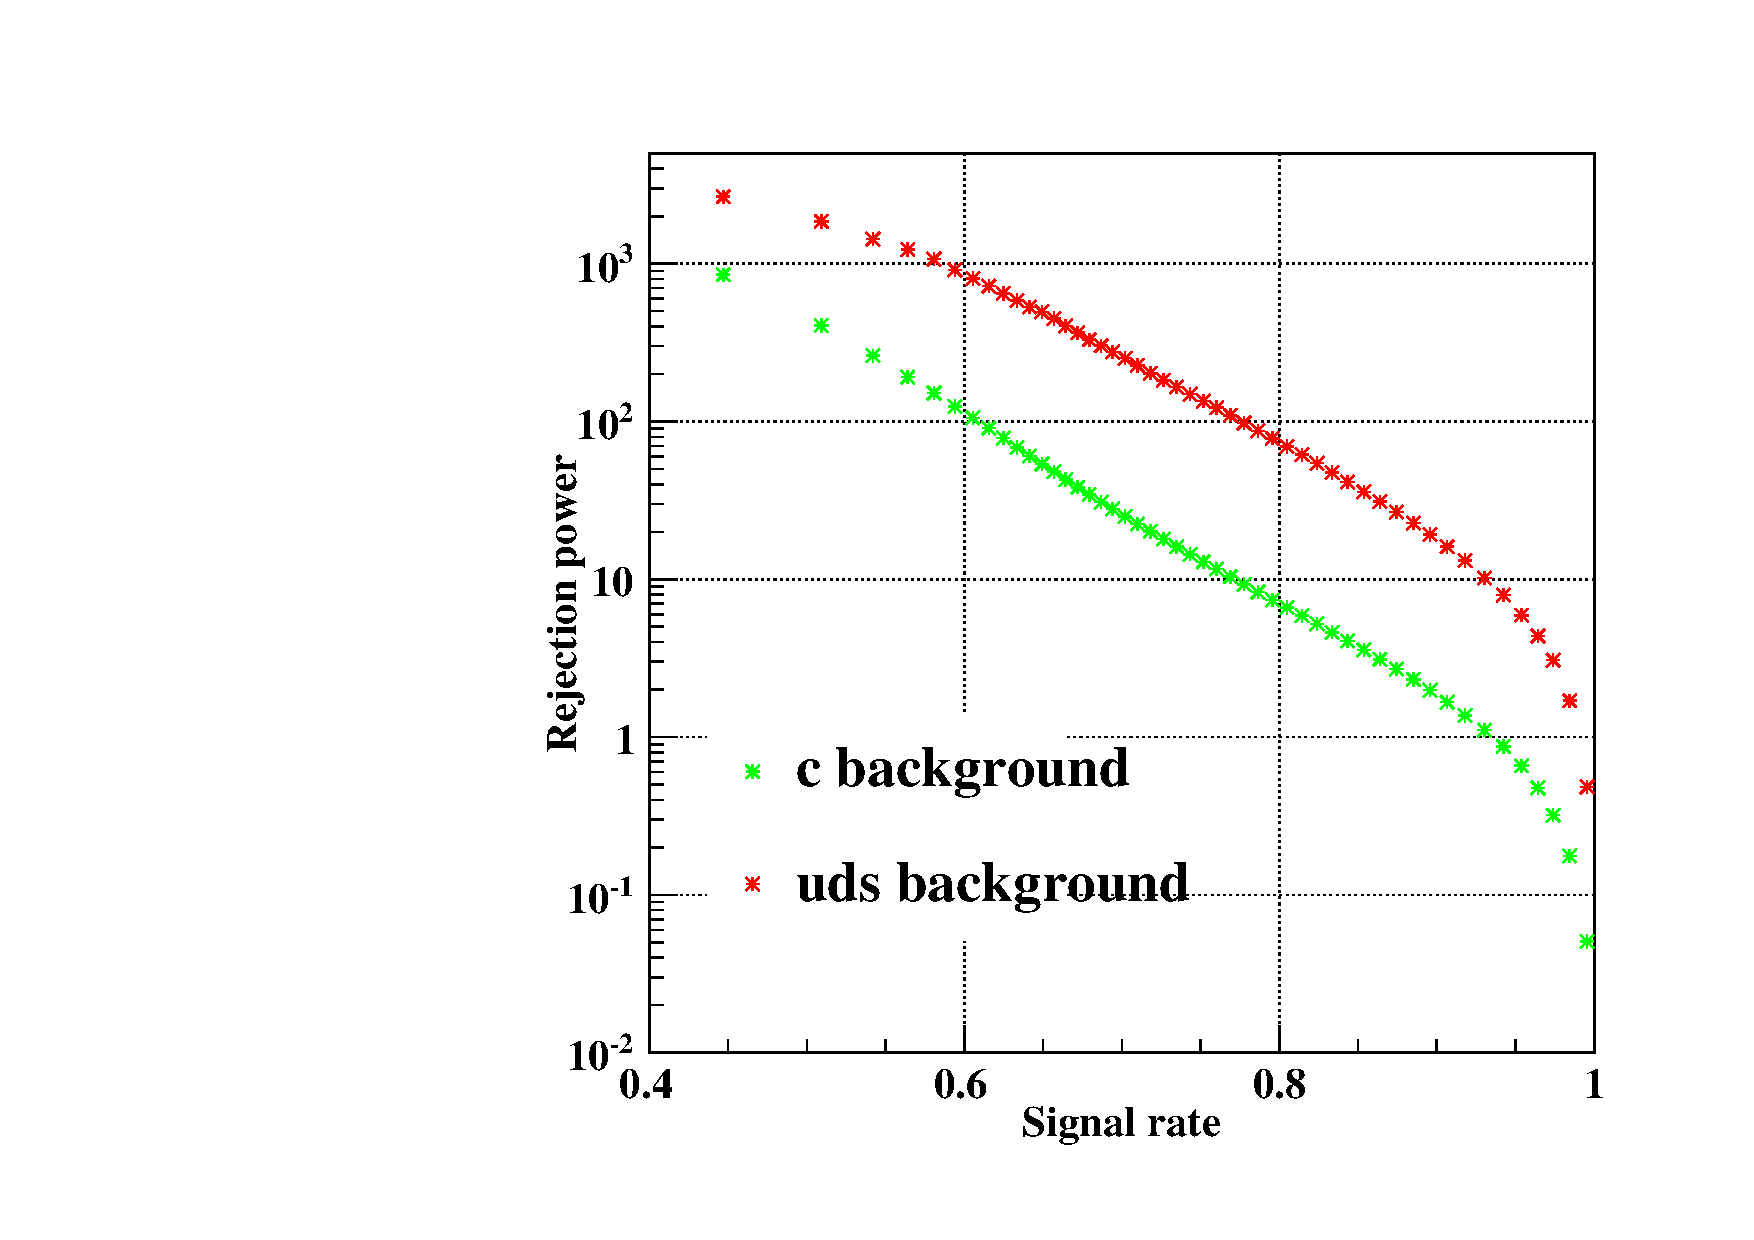
\includegraphics[width=\textwidth]{Btagging/rejectionB-lcfiweights-test.pdf}
   \end{minipage}
}
\subfigure[]
{
    \begin{minipage}[b]{0.47\textwidth}
    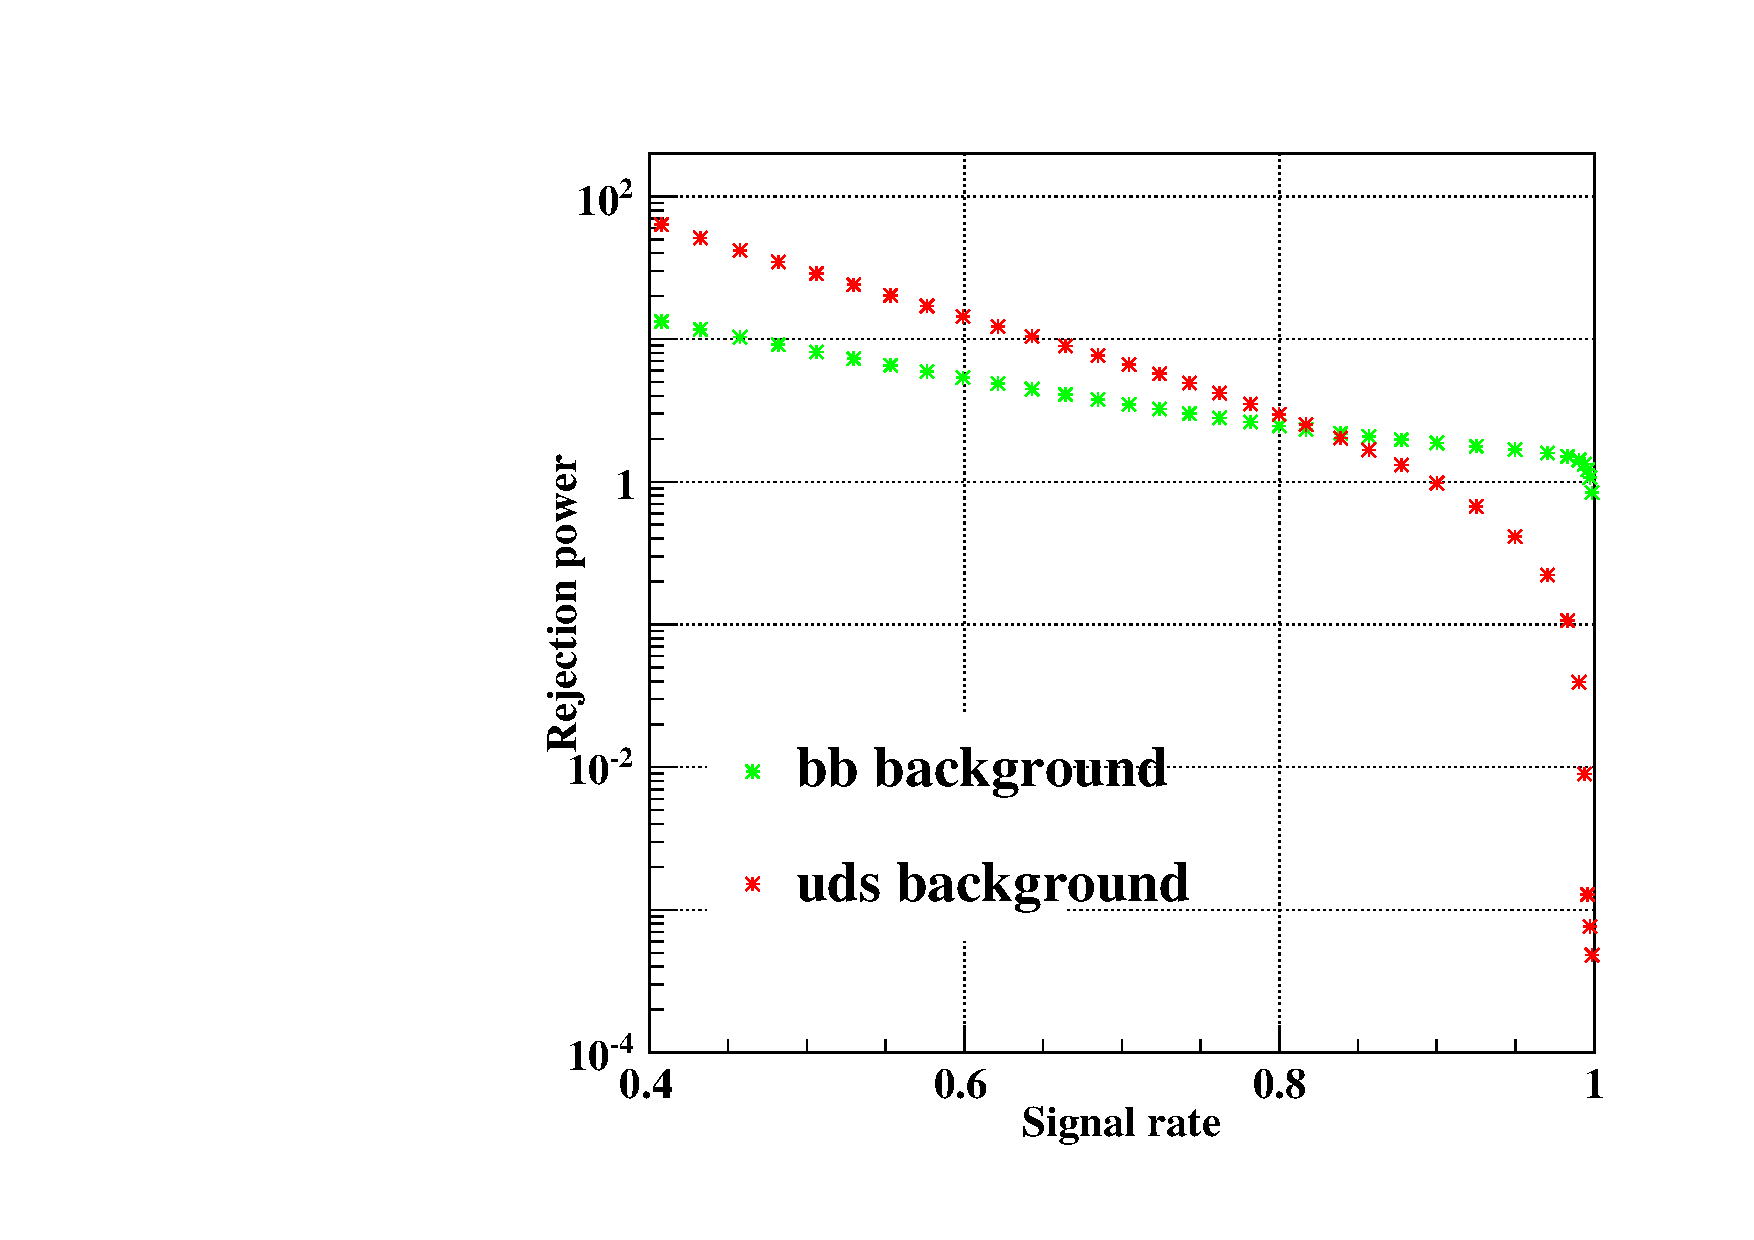
\includegraphics[width=\textwidth]{Btagging/rejectionC-lcfiweights-test.pdf}
    \end{minipage}
}
\caption{Flavor tagging performance curve. Left: b-tagging efficiency as function of rejection against $c$ and light jet. Right: c-tagging efficiency as function of rejetion against $b$ and light jet.}
\end{figure}

 
\subsection{Template fit}\label{subsec:templatefit}
 The b-likenesses of the two jets from higgs decay, say $L_{b1}$ and $L_{b2}$, can be combined to construct a discriminator variable $X_B = \dfrac{L_{b1}L_{b2}}{1-L_{b1}L_{b2}}$.  The conservation of quark flavor in higgs decay guarantee that $X_B$ is close to 1 if higgs decay to $b\bar{b}$ while close to 0 in other case. 
 Similar variable are defined for c-likeness: $X_C = \dfrac{L_{c1}L_{c2}}{1-L_{c1}L_{c2}}$. A set of template is defined according to the signal and background's $X_B-X_C$ distribution.  The $X_B-X_C$ distribution in 'data', which is composed from signal and background simulation events, is shown in figure \ref{fig:data_template}.
 \begin{figure}[!htpb]
 \label{fig:data_template}
 \centering
 \subfigure[]
{
  \begin{minipage}[b]{0.42\textwidth}
  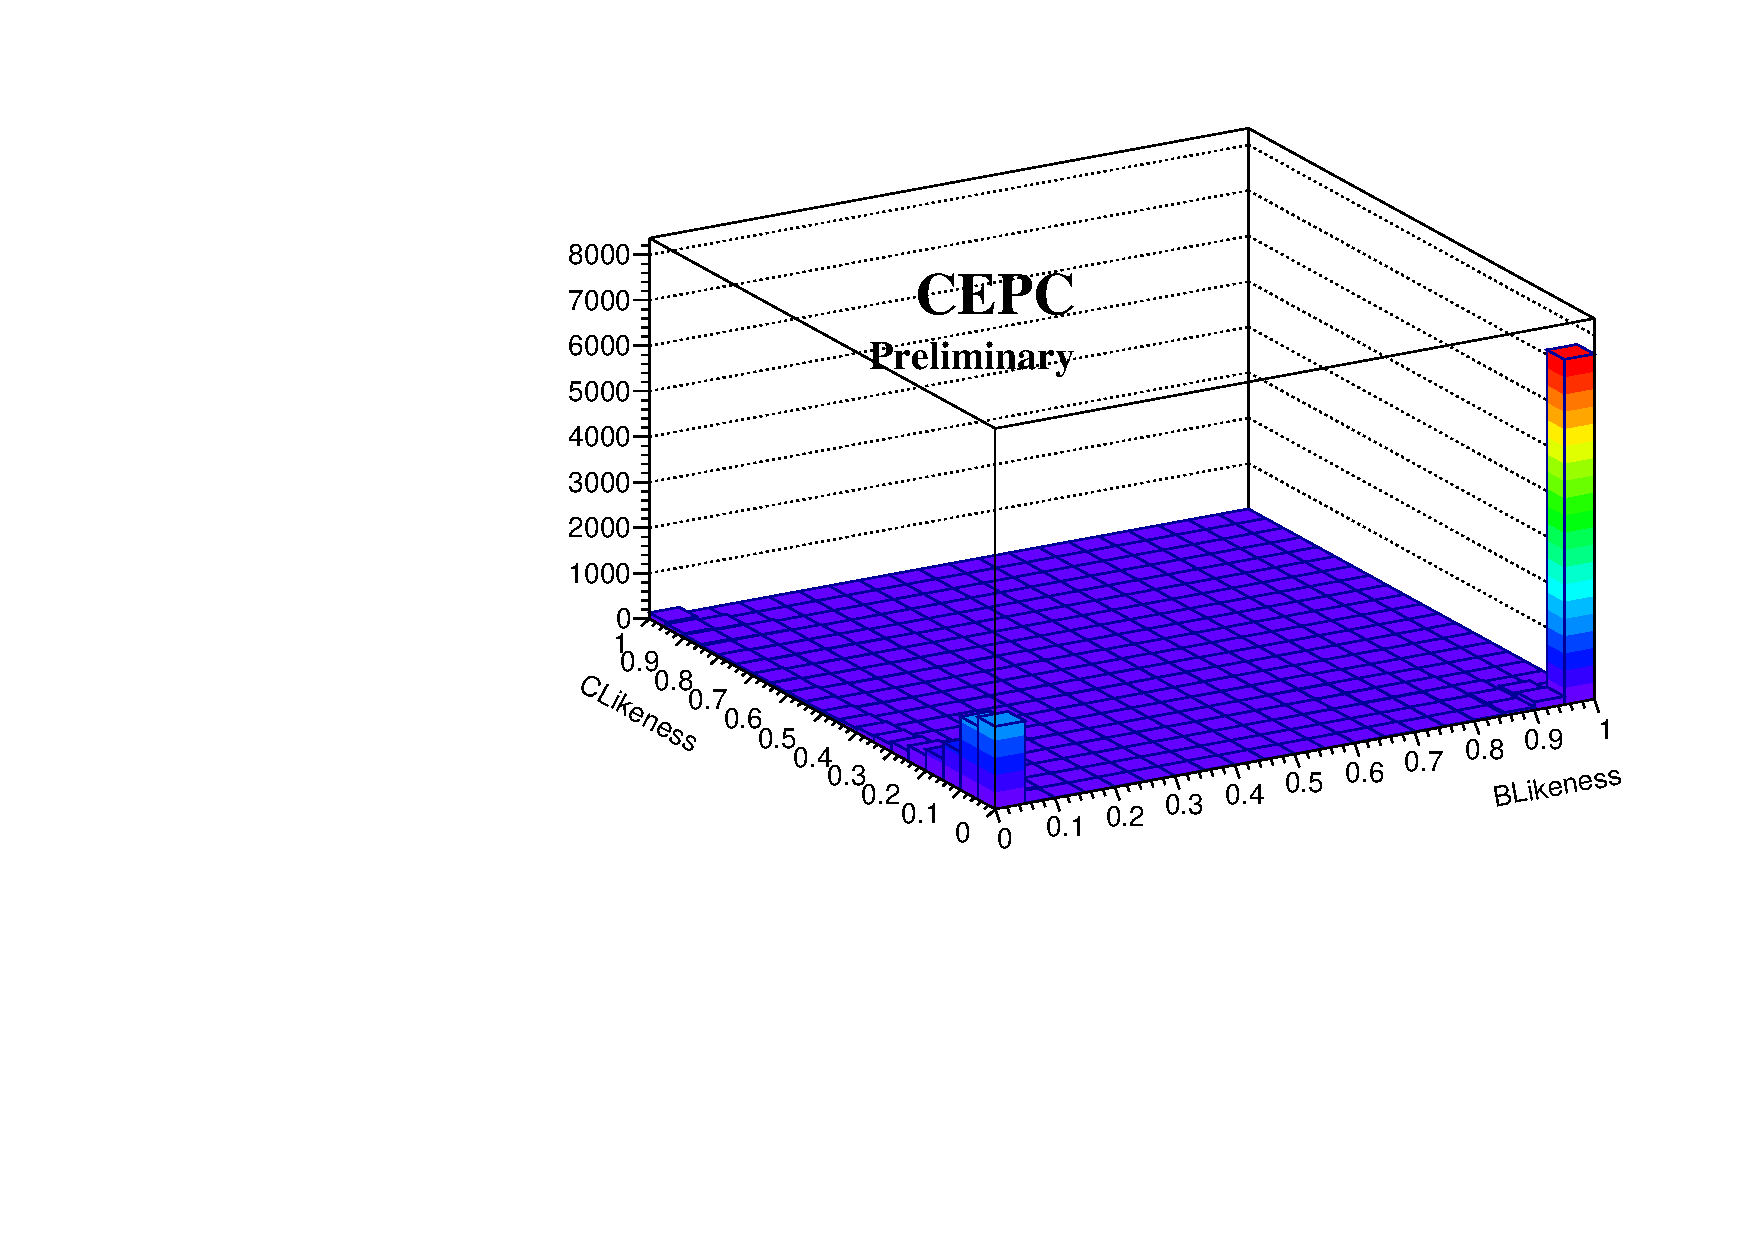
\includegraphics[width=\textwidth]{Template/eeh_data.pdf}
  \end{minipage}
}
\subfigure[]
{
  \begin{minipage}[b]{0.42\textwidth}
  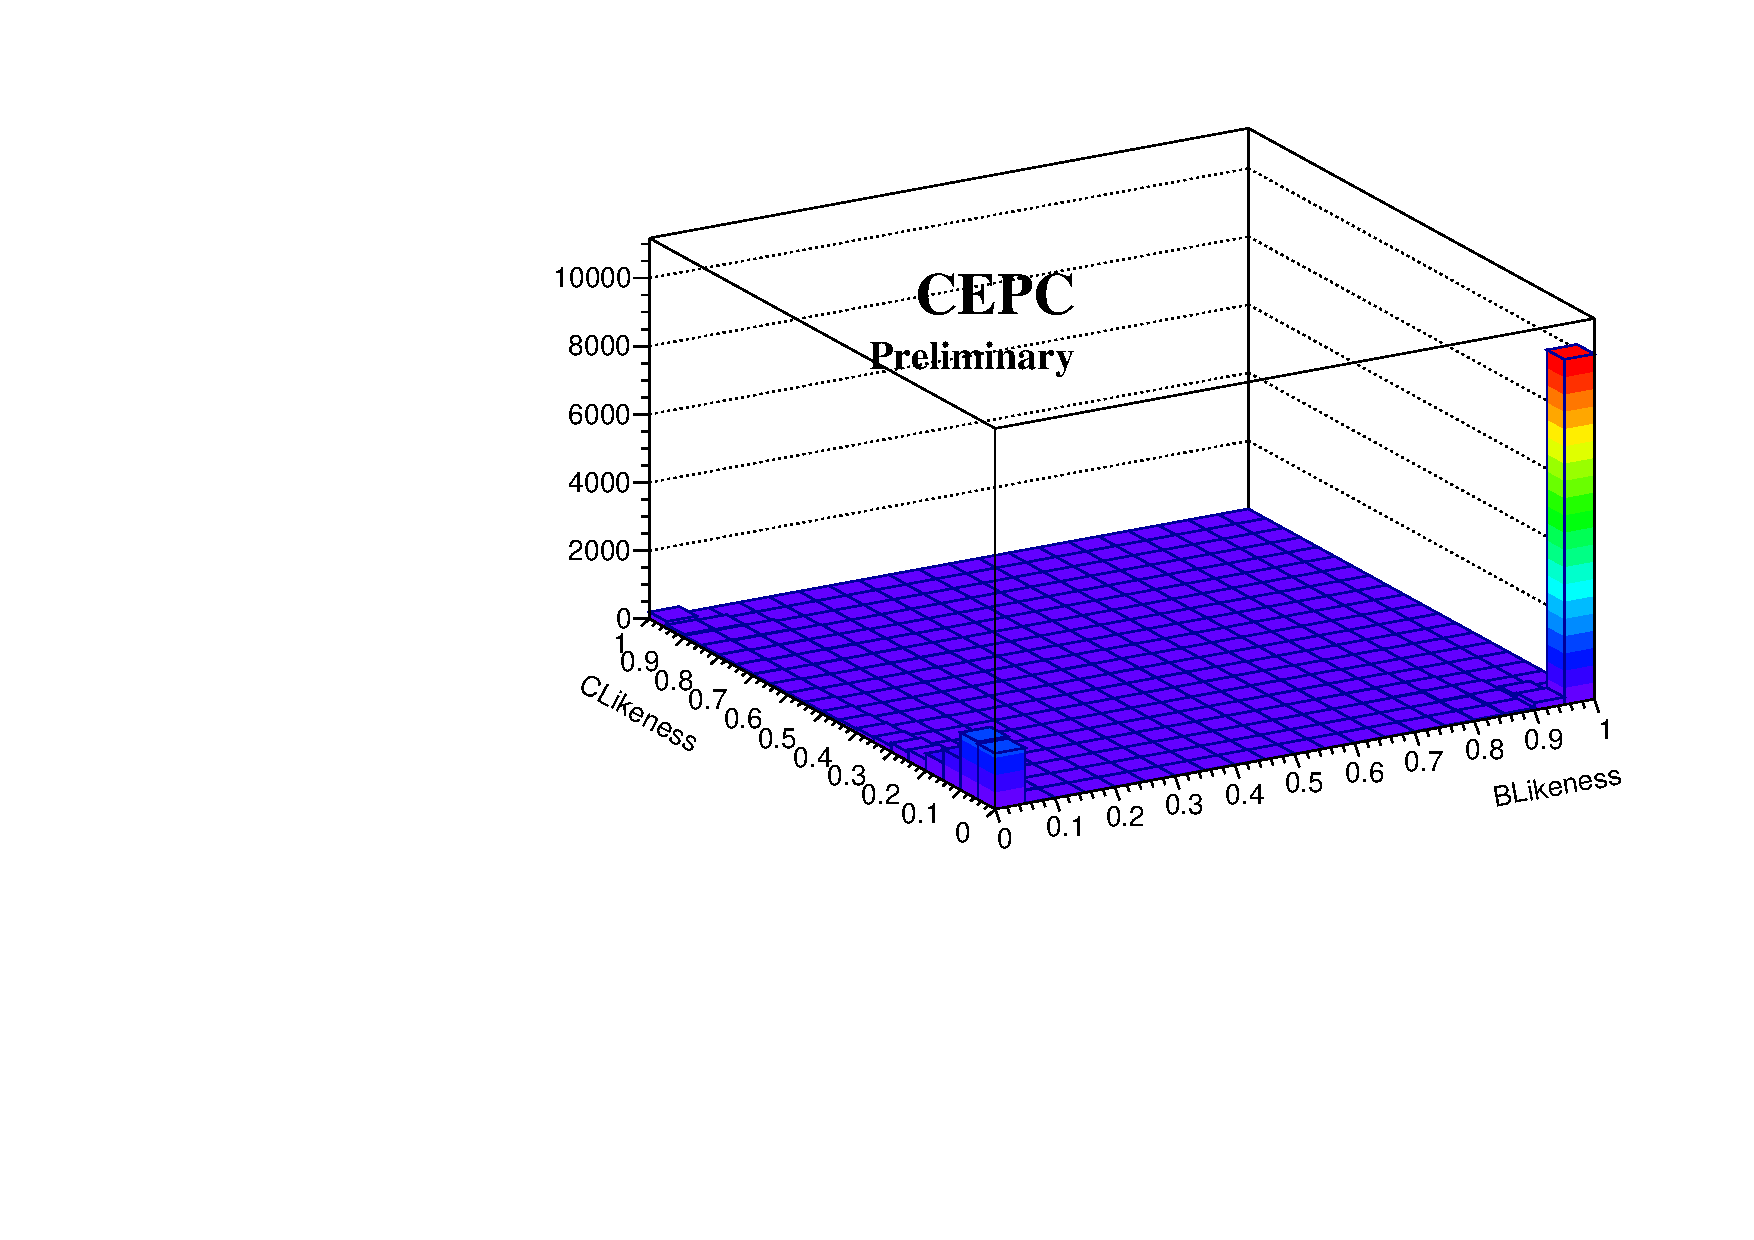
\includegraphics[width=\textwidth]{Template/mumuh_data.pdf}
  \end{minipage}
}
\subfigure[]
{ 
   \begin{minipage}[b]{0.42\textwidth}
   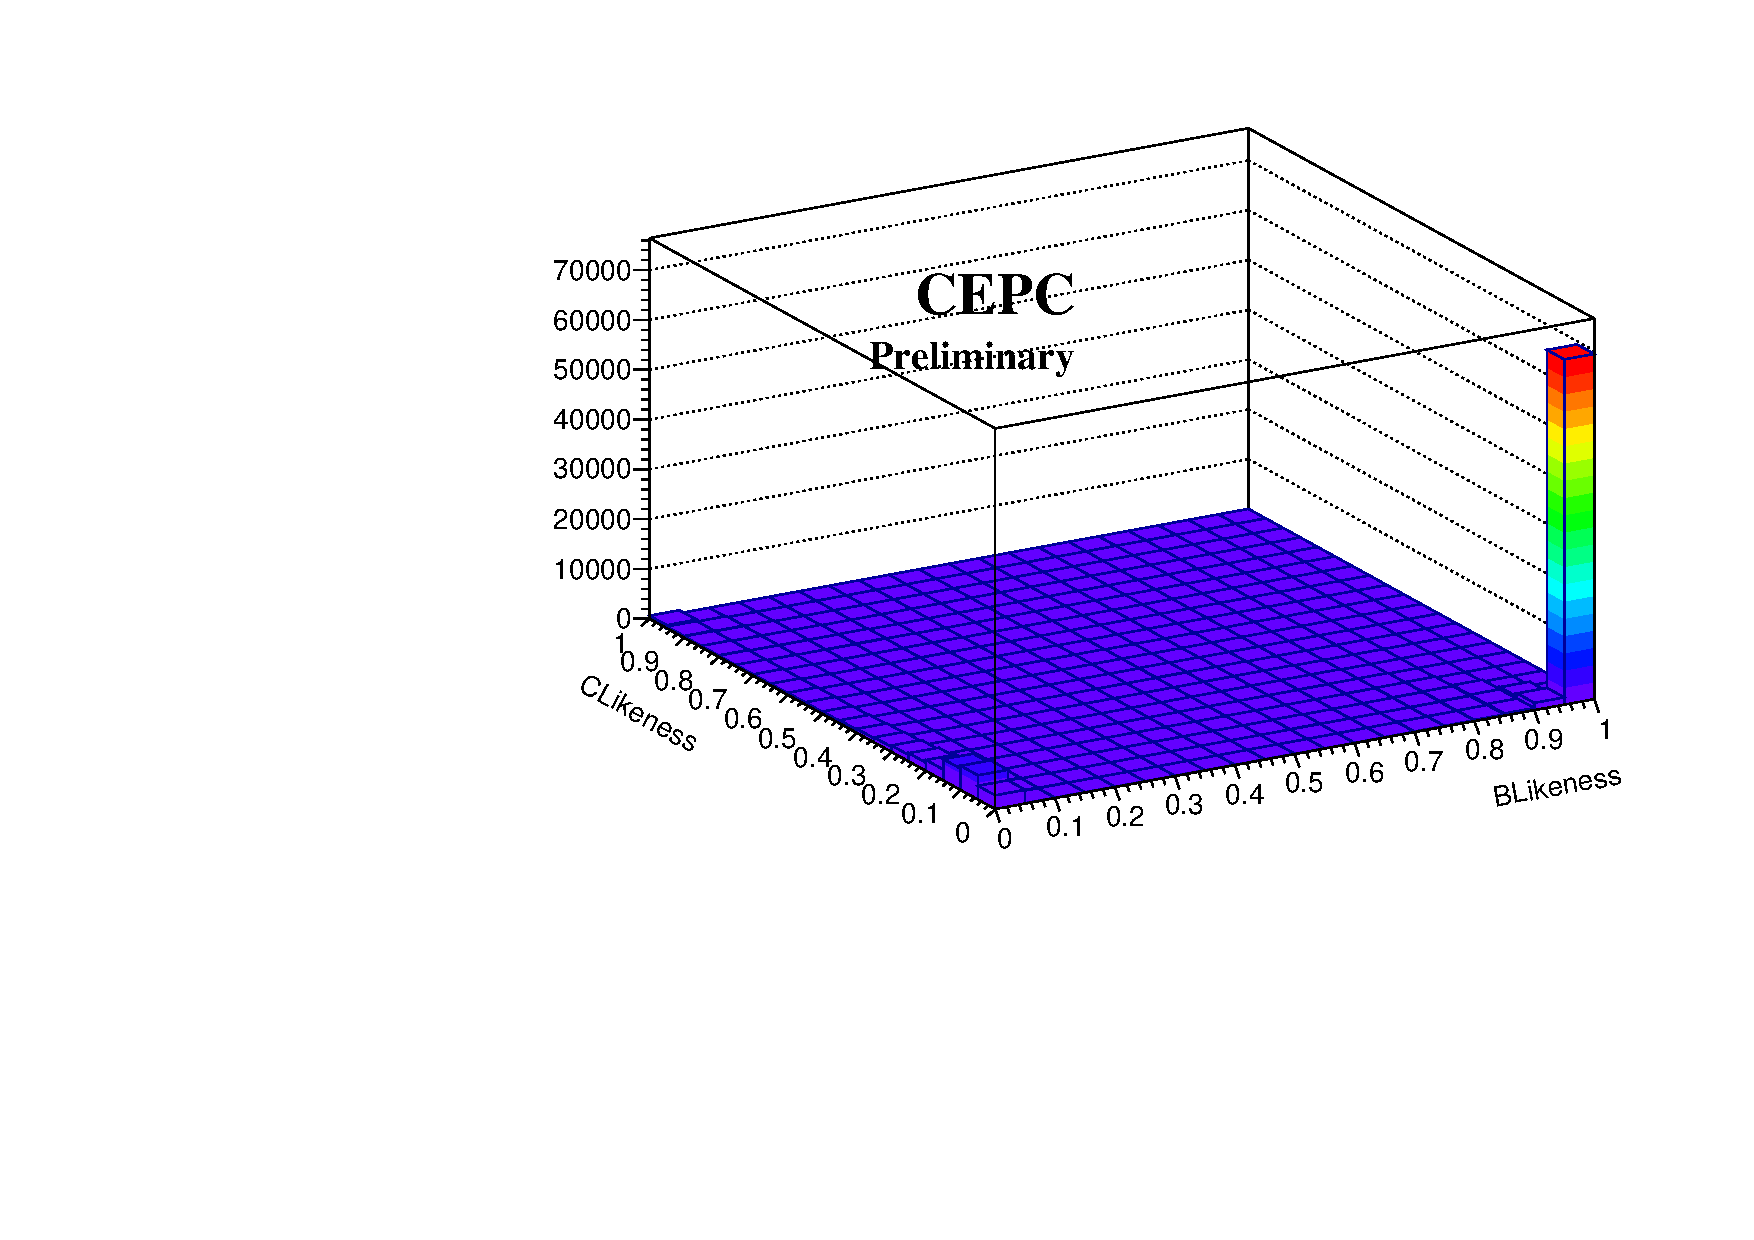
\includegraphics[width=\textwidth]{Template/nnh_data.pdf}
   \end{minipage}
}
\subfigure[]
{
    \begin{minipage}[b]{0.42\textwidth}
    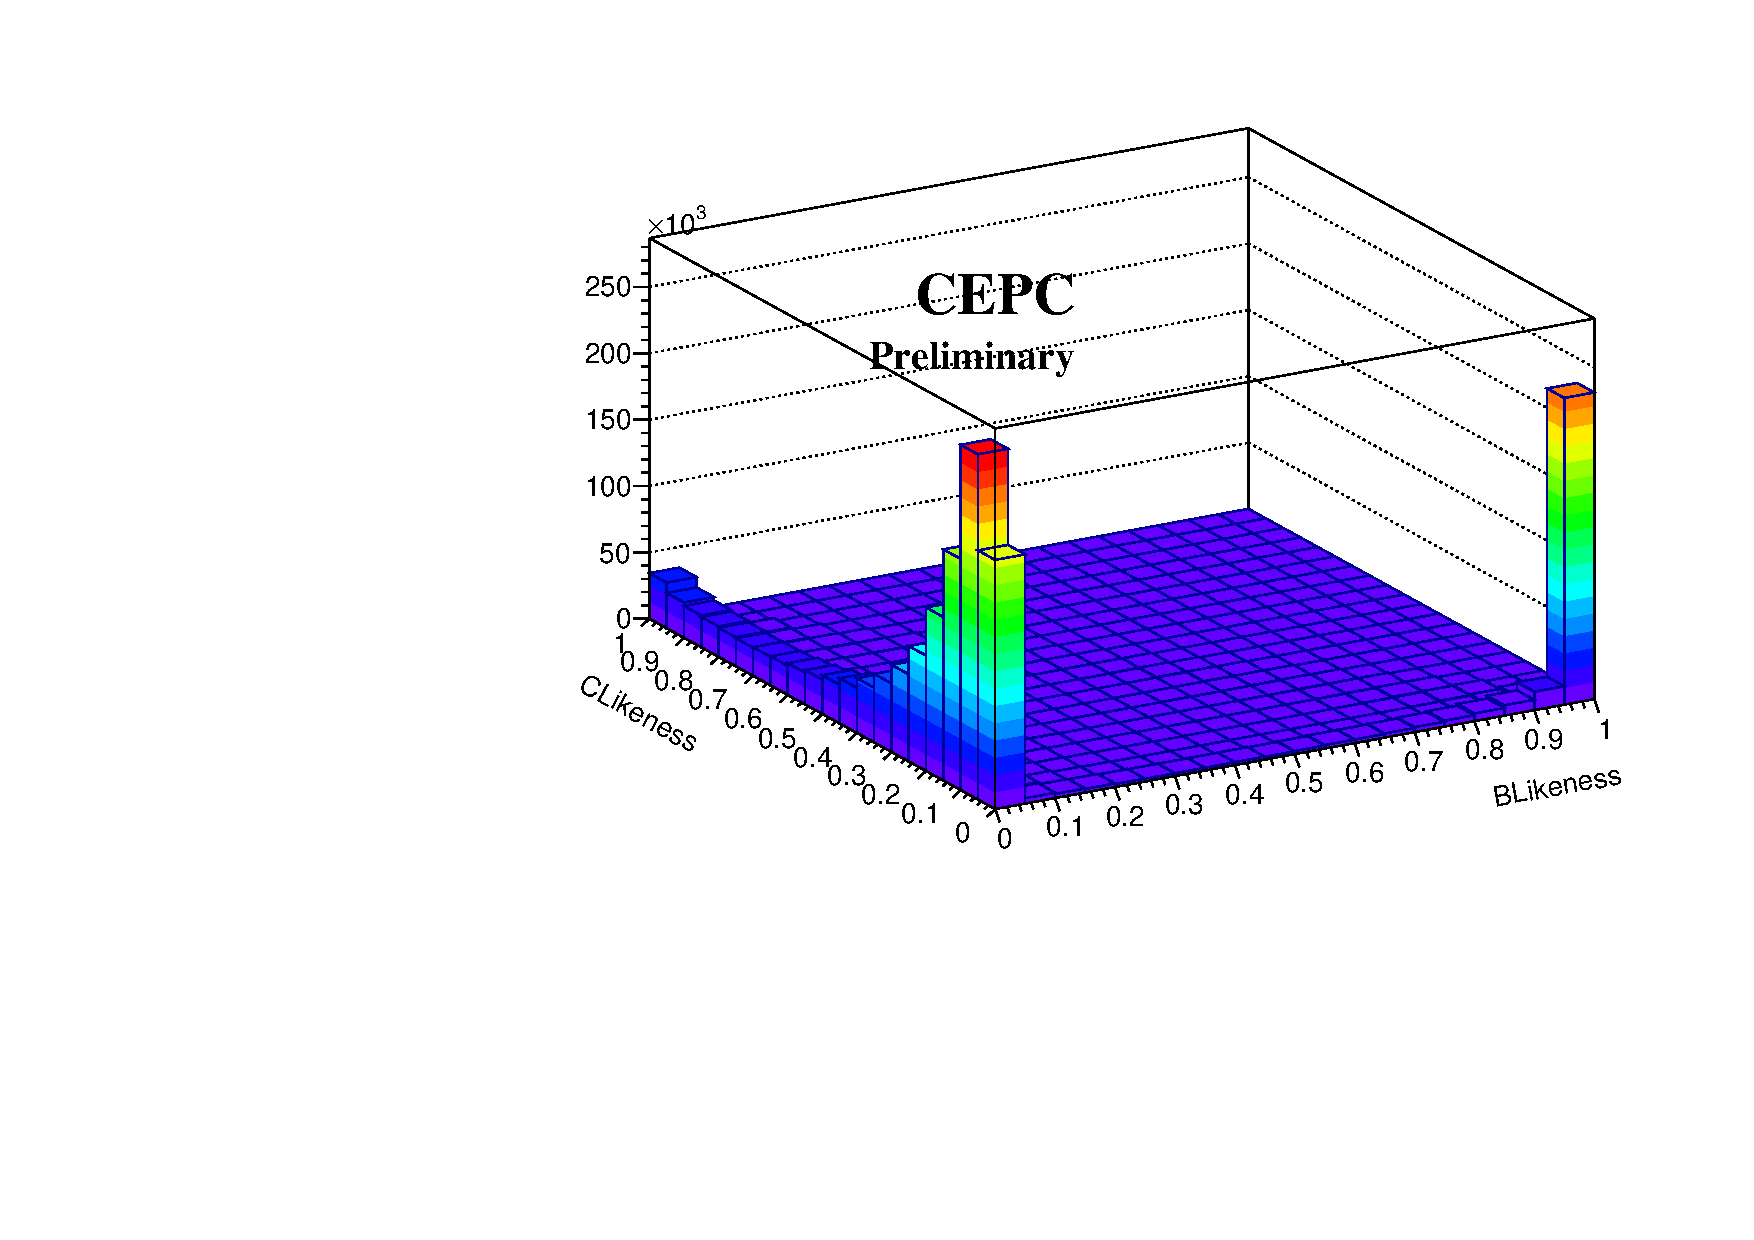
\includegraphics[width=\textwidth]{Template/qqh_data.pdf}
    \end{minipage}
}
 \caption{$X_B-X_C$ distribution of pesudo-data in each channel: templates of \eeh(top left),\mmh(top right),\nnh(bottom left) and \qqh(bottom right)}
 \end{figure}

 A likelihood was constructed according to the template distribution:
 \begin{equation}
 \log{L} = \sum\limits_{i=1}^N{\log{Possion(\mu_{i},n_{i})}}
 \label{for:template}
 \end{equation}
in which i is the bin index(we have 20 bins for $X_B$ and $X_C$ so in all $N=400$); $Possion(\mu_{i},n_{i})$ is the Possion likelihood with for $n_{i}$ obvserved event and expectation $\mu_{i}$, which include the parameter of interest:
\begin{equation}
\mu_{i} = \sum\limits_{j=1}^s f_j\times\mu_{i,j}
\end{equation}
in which j is the index of templates (one template for each components); $f_j$ is the fraction of $j$th components which need to be worked out; $\mu_{i,j}$ stands for the expected event yields of $j$th components in $i$th bin. Minimize $-\log{L}$ we can fit the $f_j$. The distribution of template for $H\to gg/bb/cc$ is shown in figure \ref{fig:sig_template}. The $\Hboson \to \bpair$ and $\Hboson \to\cpair$ concentrate in region (1,0) and (0,1) respectively, while $\Hboson\to\gpair$ tends to distribute around (0,0). It can be found a tail at (1,0) show up in $\Hboson$ distribution, which are due to contribution of gluon splitting $g\to \bpair$(\eeh,\mmh and \nnh) and hadronic $Z-$decay(\qqh).
 
\begin{figure}[!htpb]
\label{fig:sig_template}
\centering
\subfigure[]
{
  \begin{minipage}[b]{0.33\textwidth}
  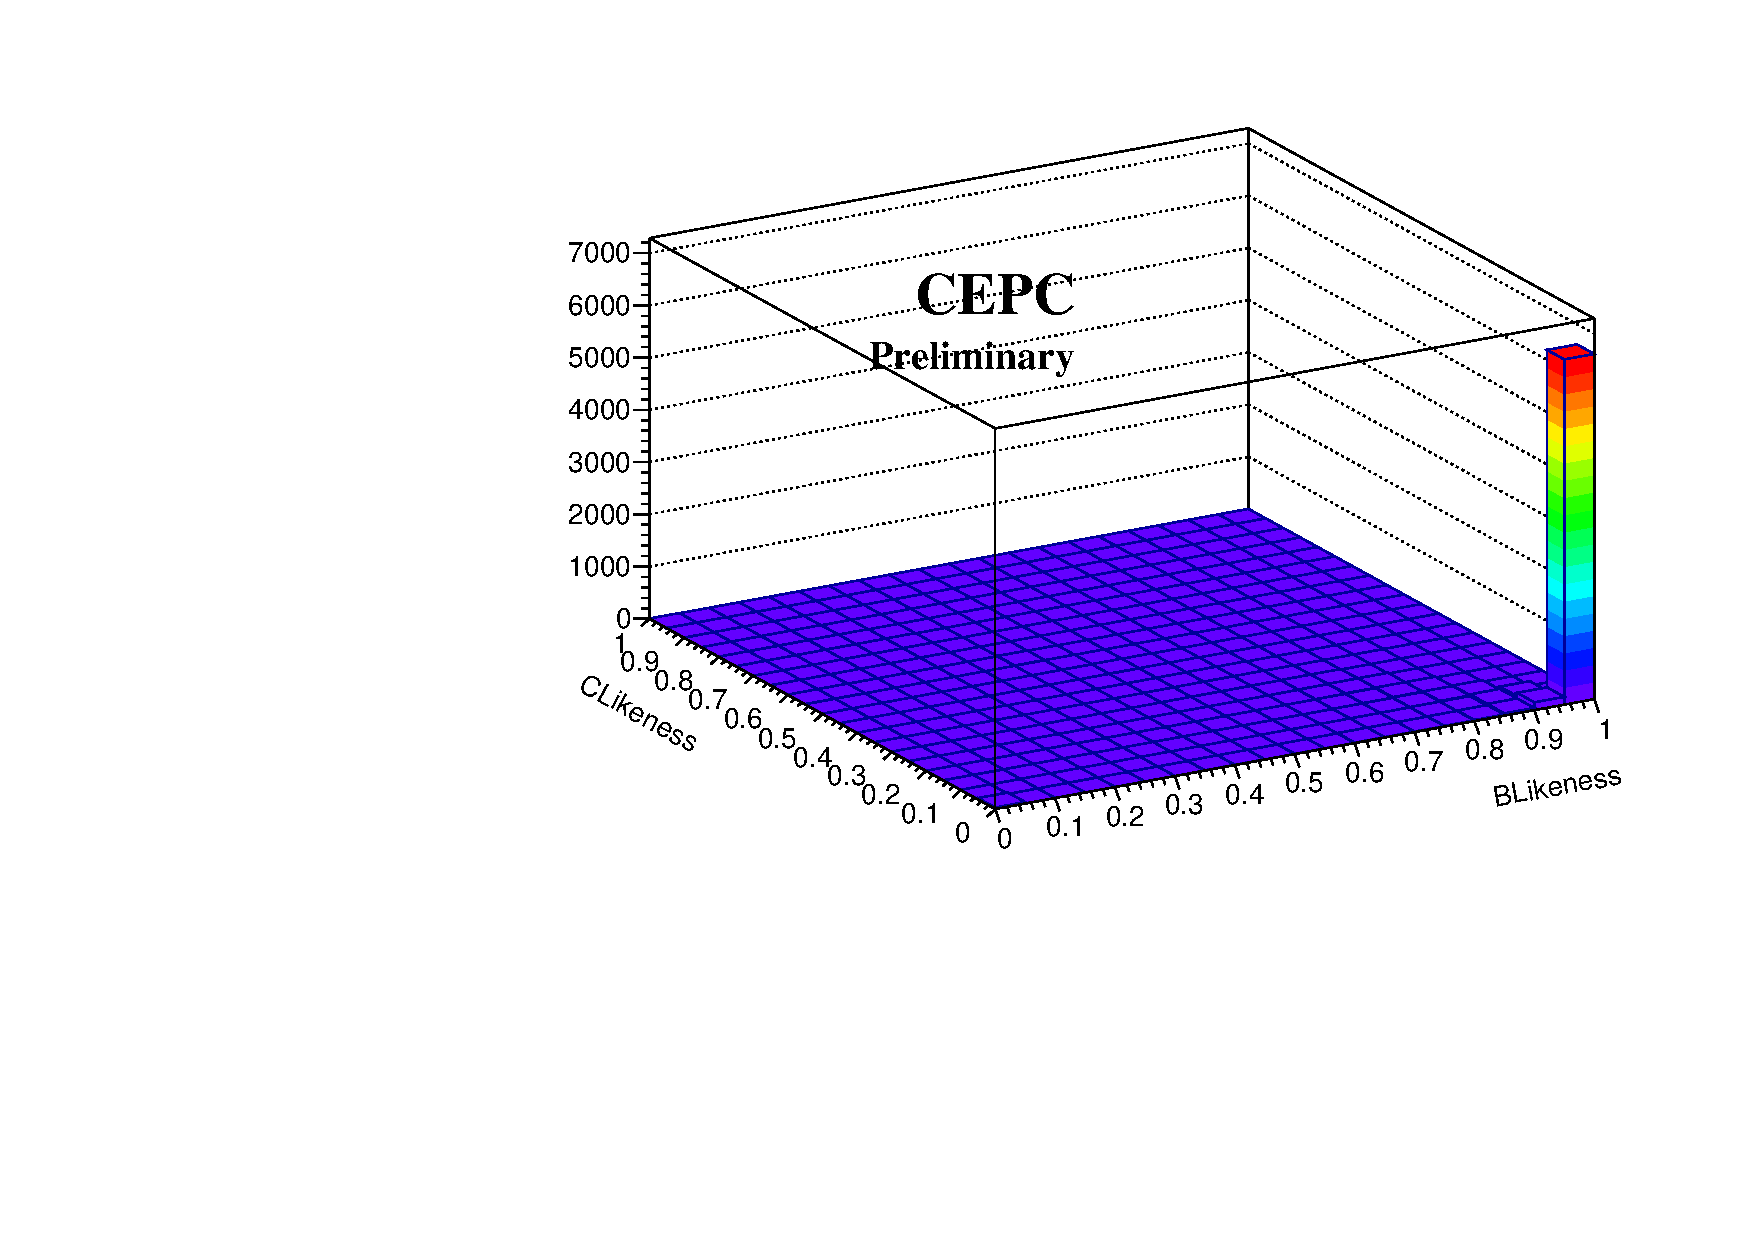
\includegraphics[width=\textwidth]{Template/eeh_bb.pdf}
  \end{minipage}
}
\subfigure[]
{
  \begin{minipage}[b]{0.31\textwidth}
  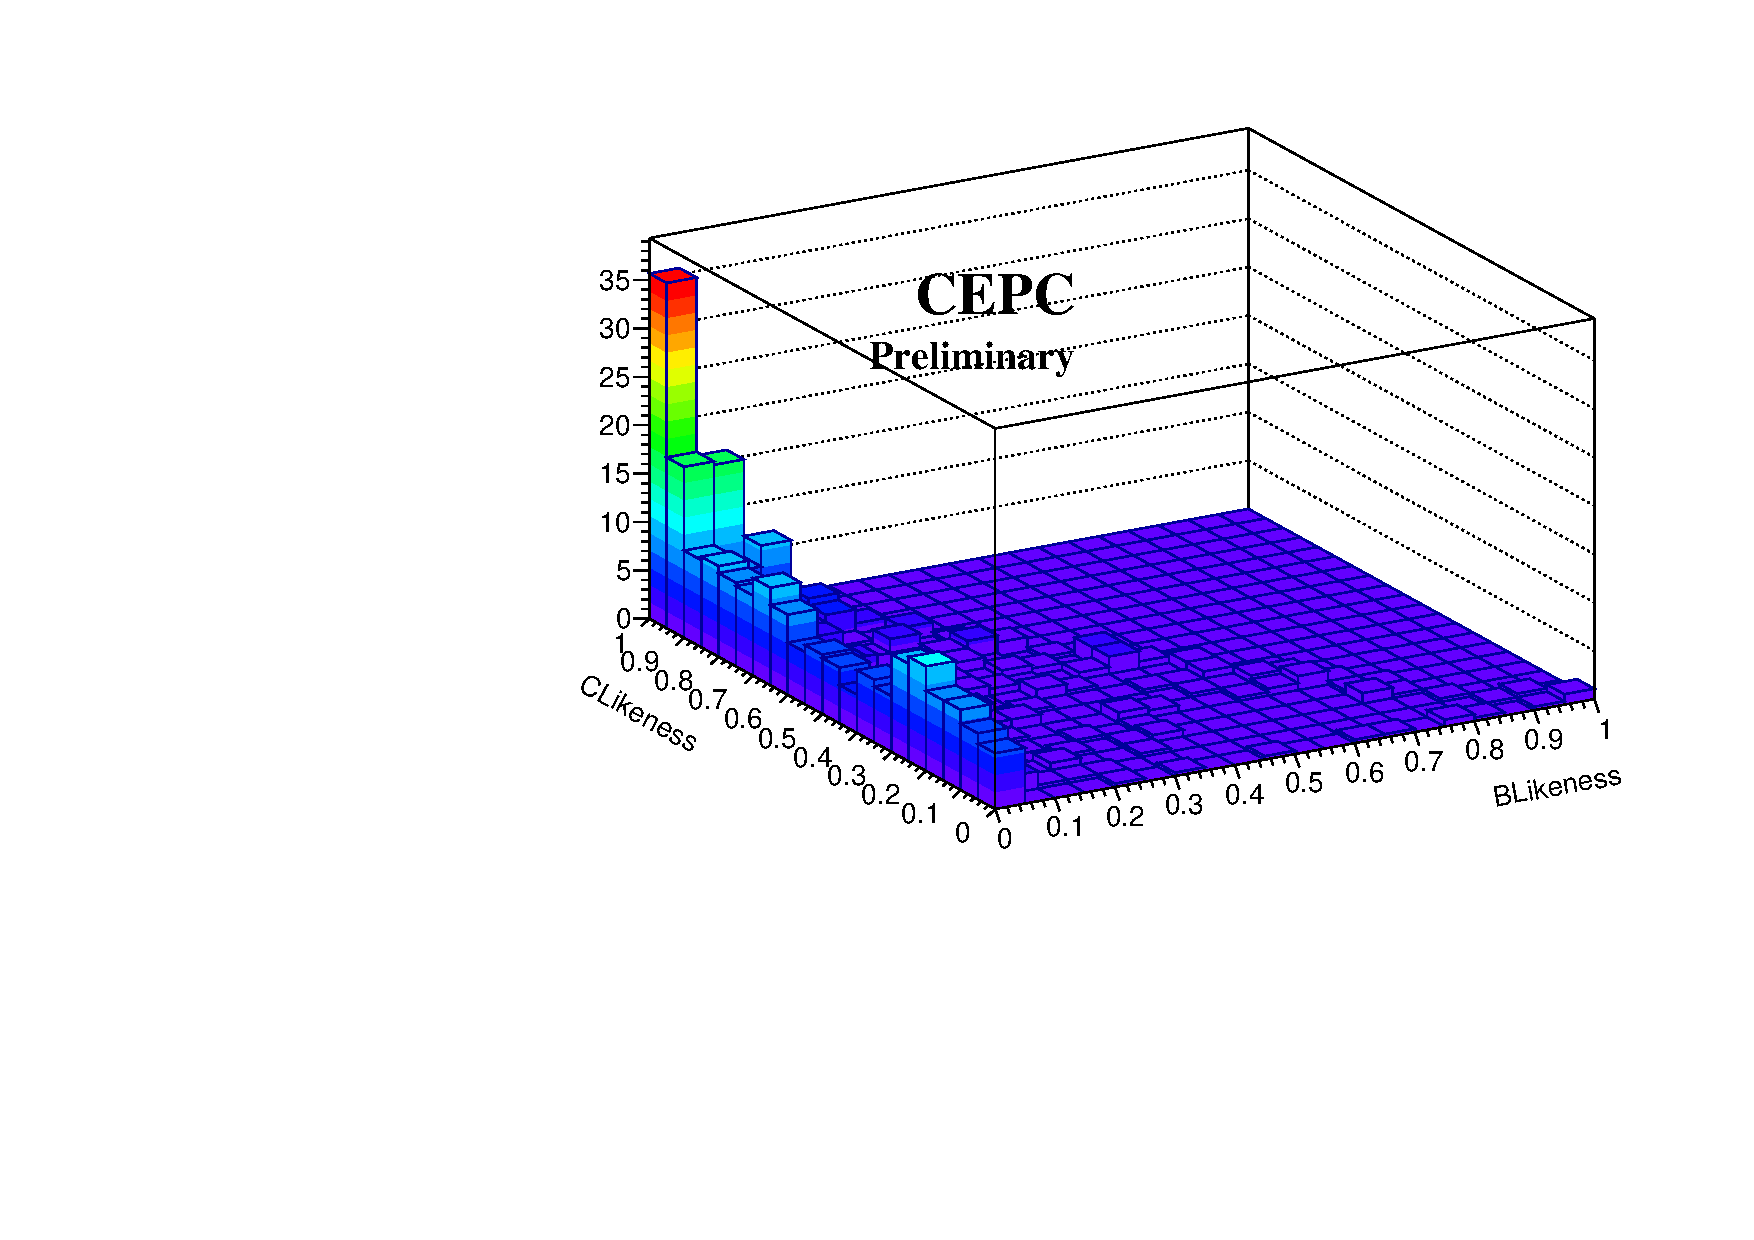
\includegraphics[width=\textwidth]{Template/eeh_cc.pdf}
  \end{minipage}
}
\subfigure[]
{ 
   \begin{minipage}[b]{0.31\textwidth}
   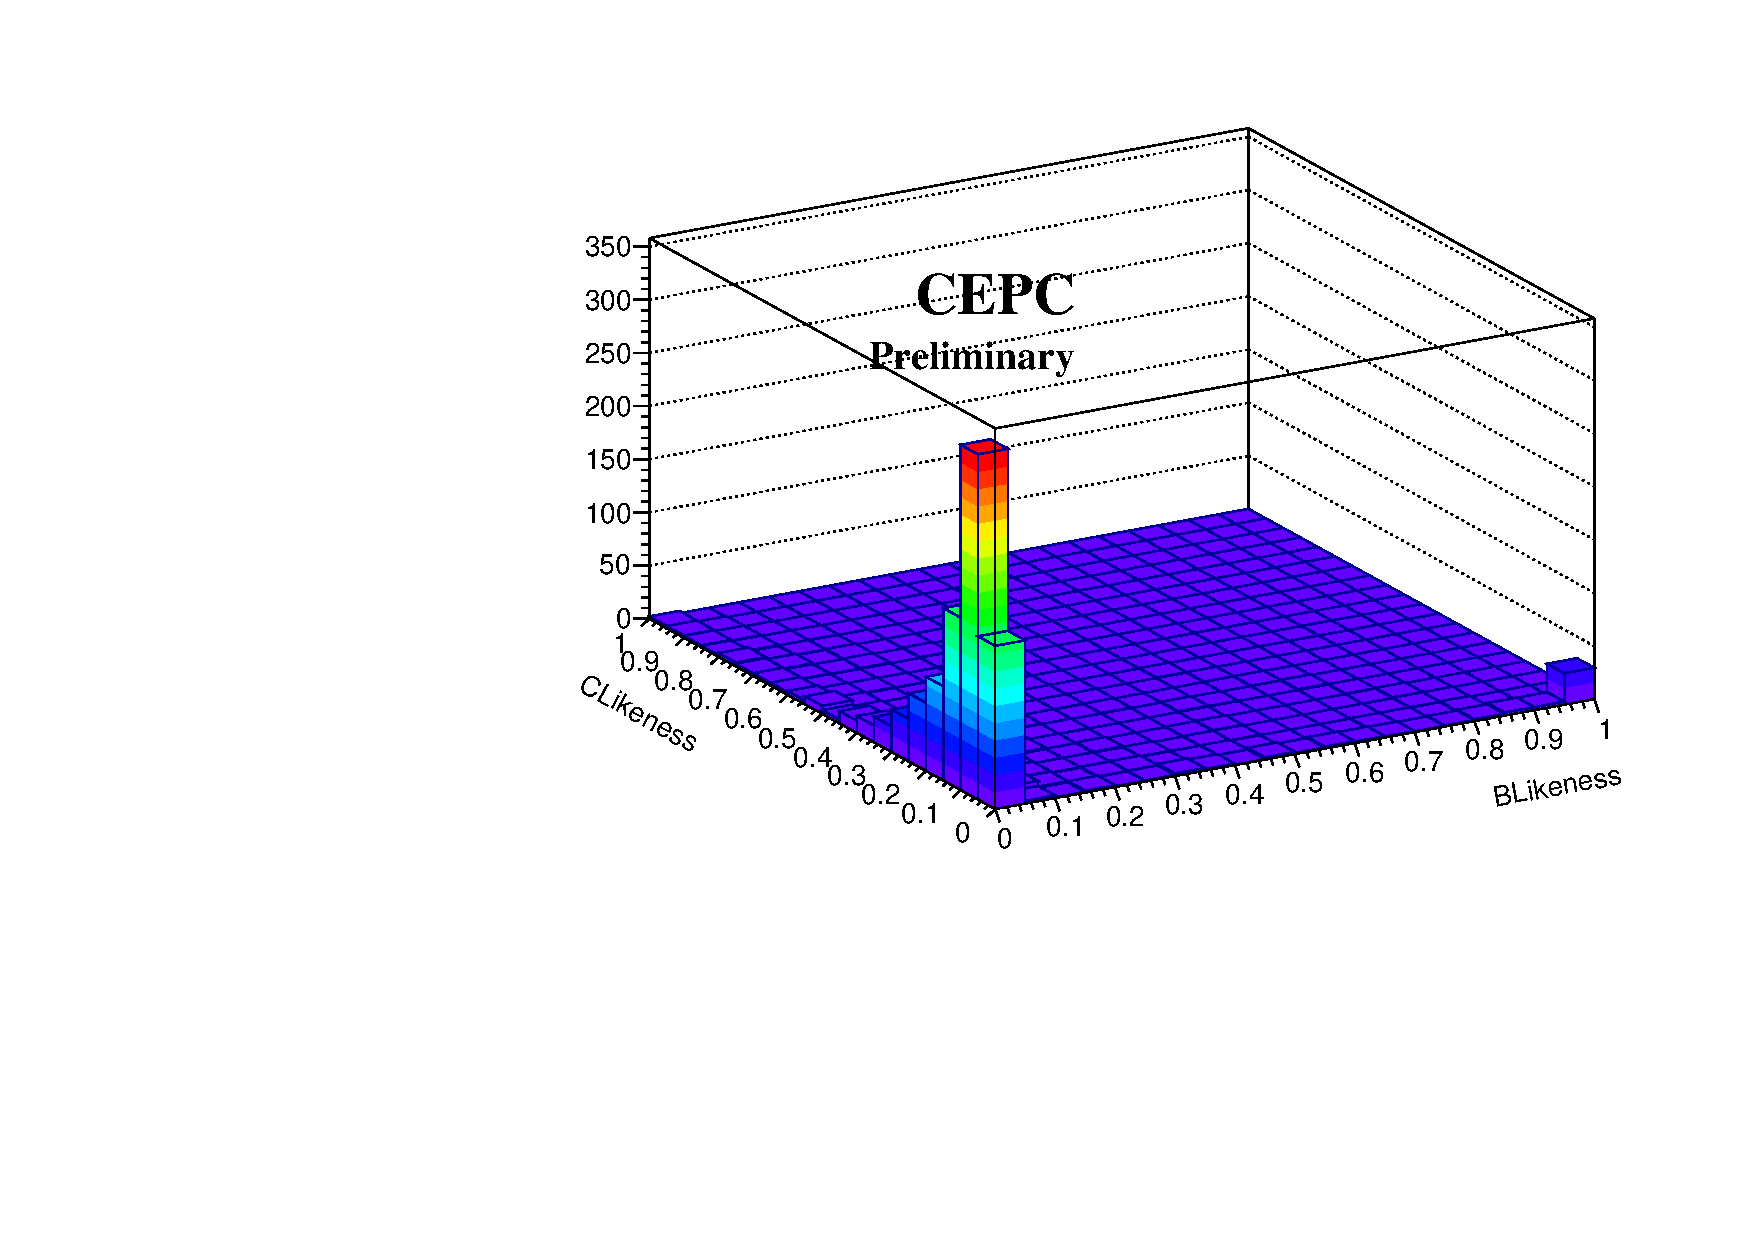
\includegraphics[width=\textwidth]{Template/eeh_gg.pdf}
   \end{minipage}
}
\subfigure[]
{
    \begin{minipage}[b]{0.31\textwidth}
    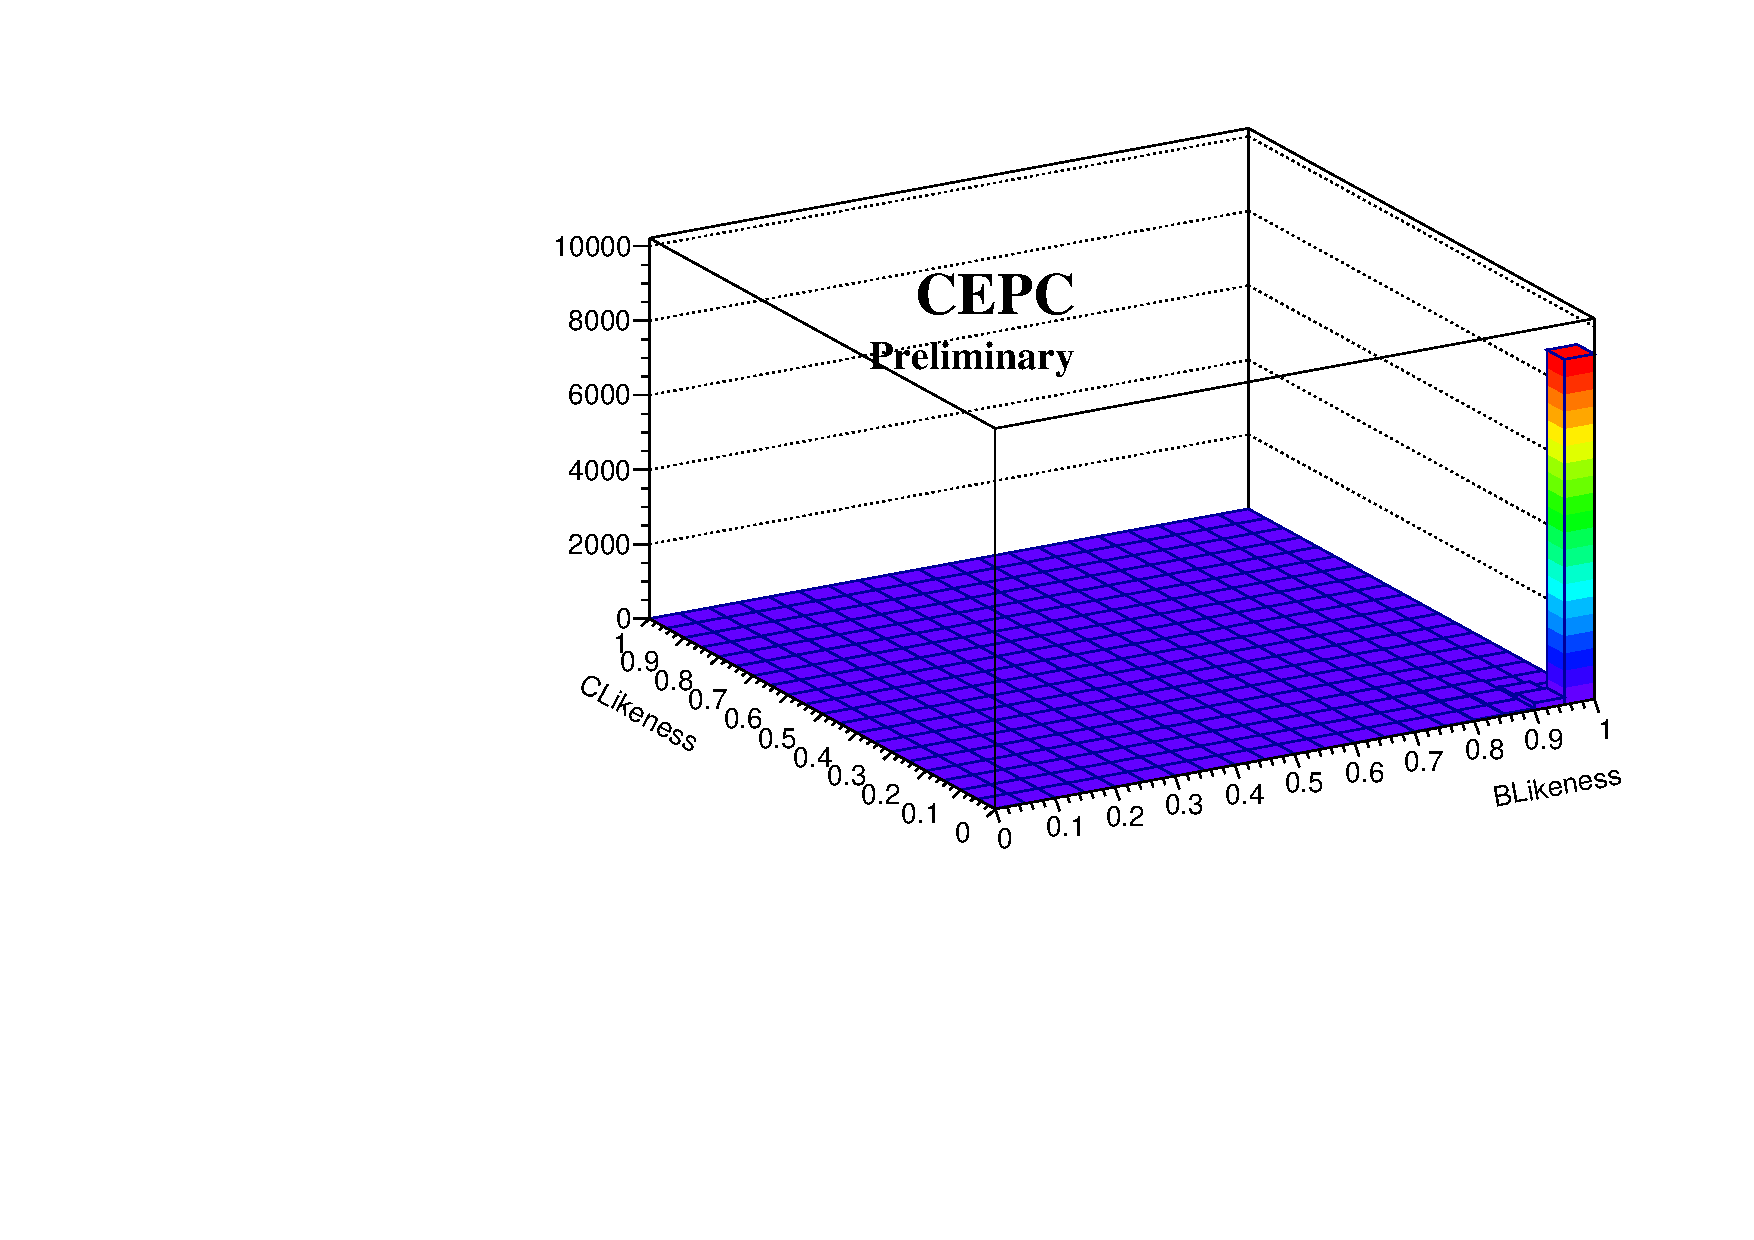
\includegraphics[width=\textwidth]{Template/mumuh_bb.pdf}
    \end{minipage}
}
\subfigure[]
{ 
   \begin{minipage}[b]{0.31\textwidth}
   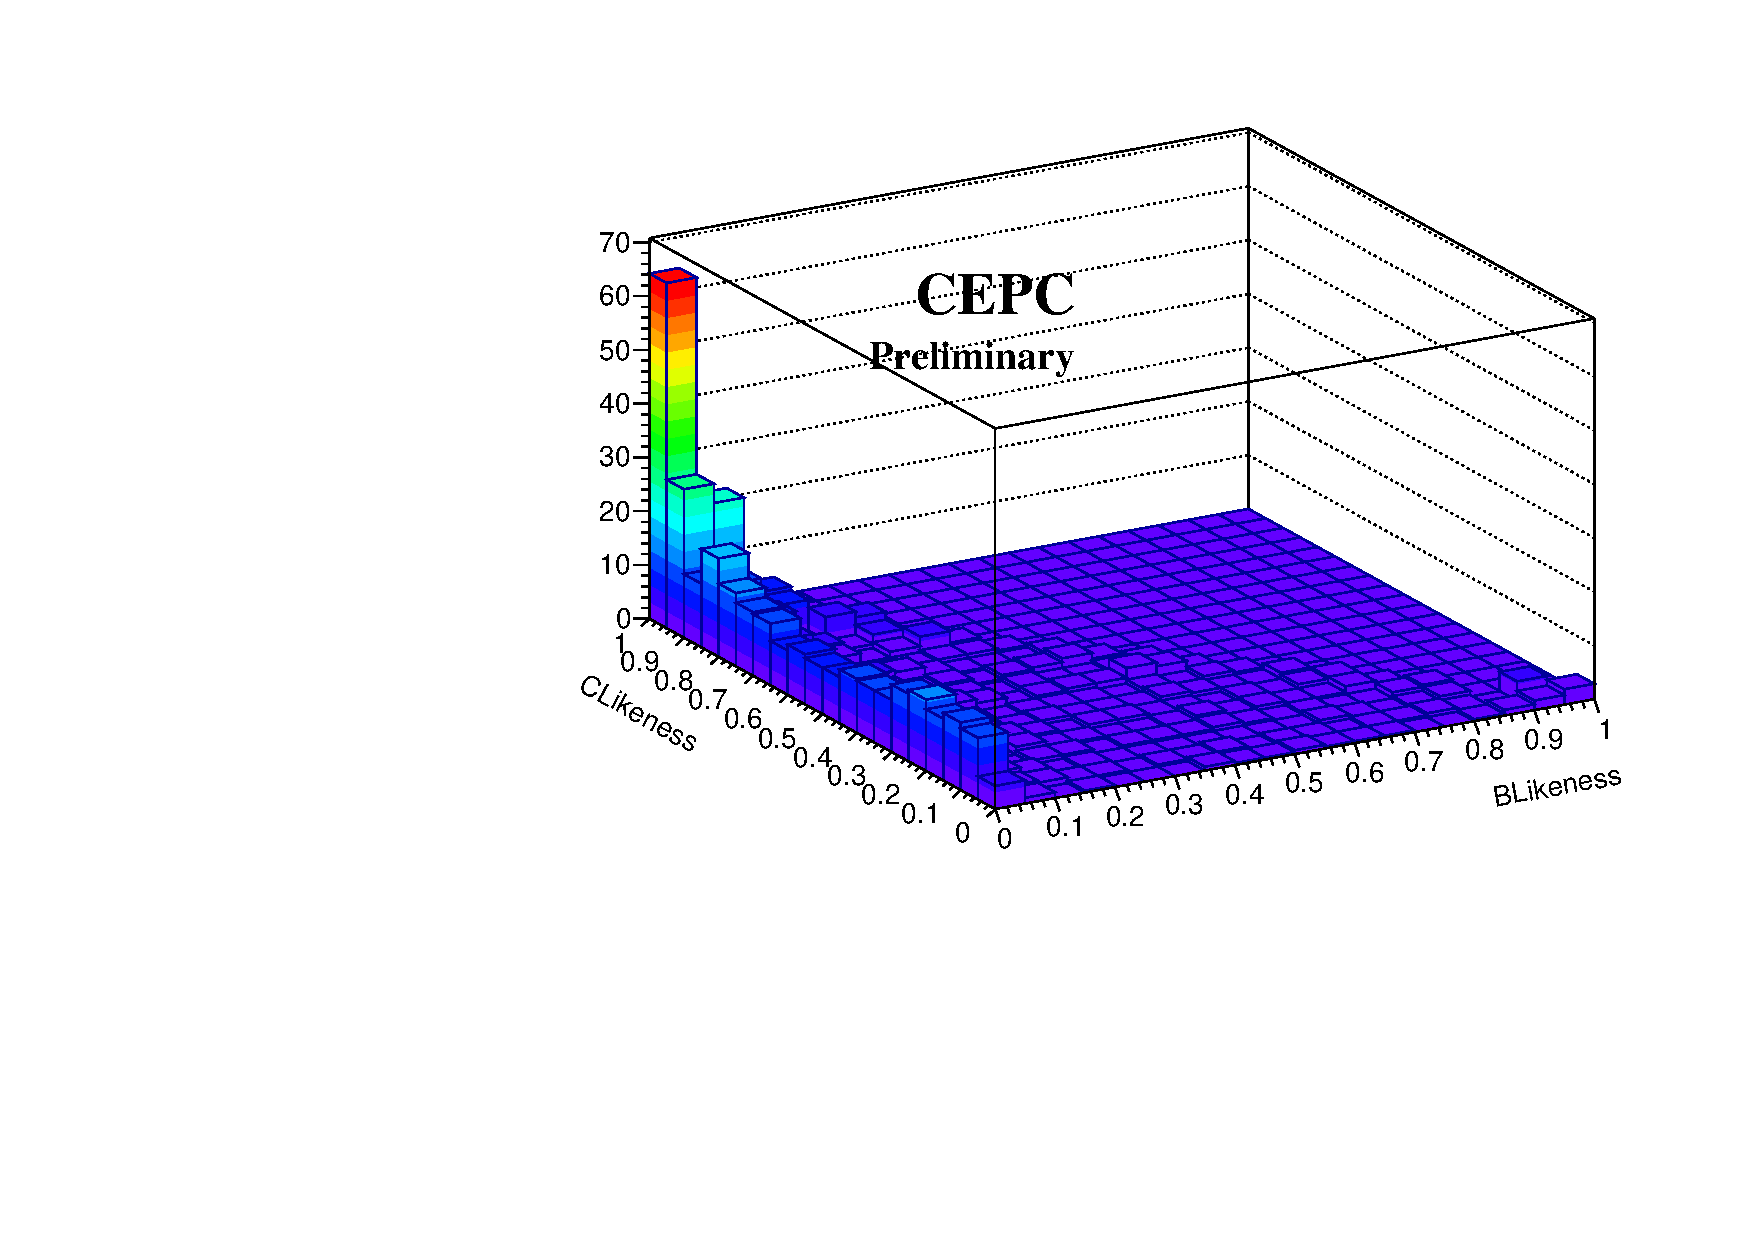
\includegraphics[width=\textwidth]{Template/mumuh_cc.pdf}
   \end{minipage}
}
\subfigure[]
{
    \begin{minipage}[b]{0.31\textwidth}
    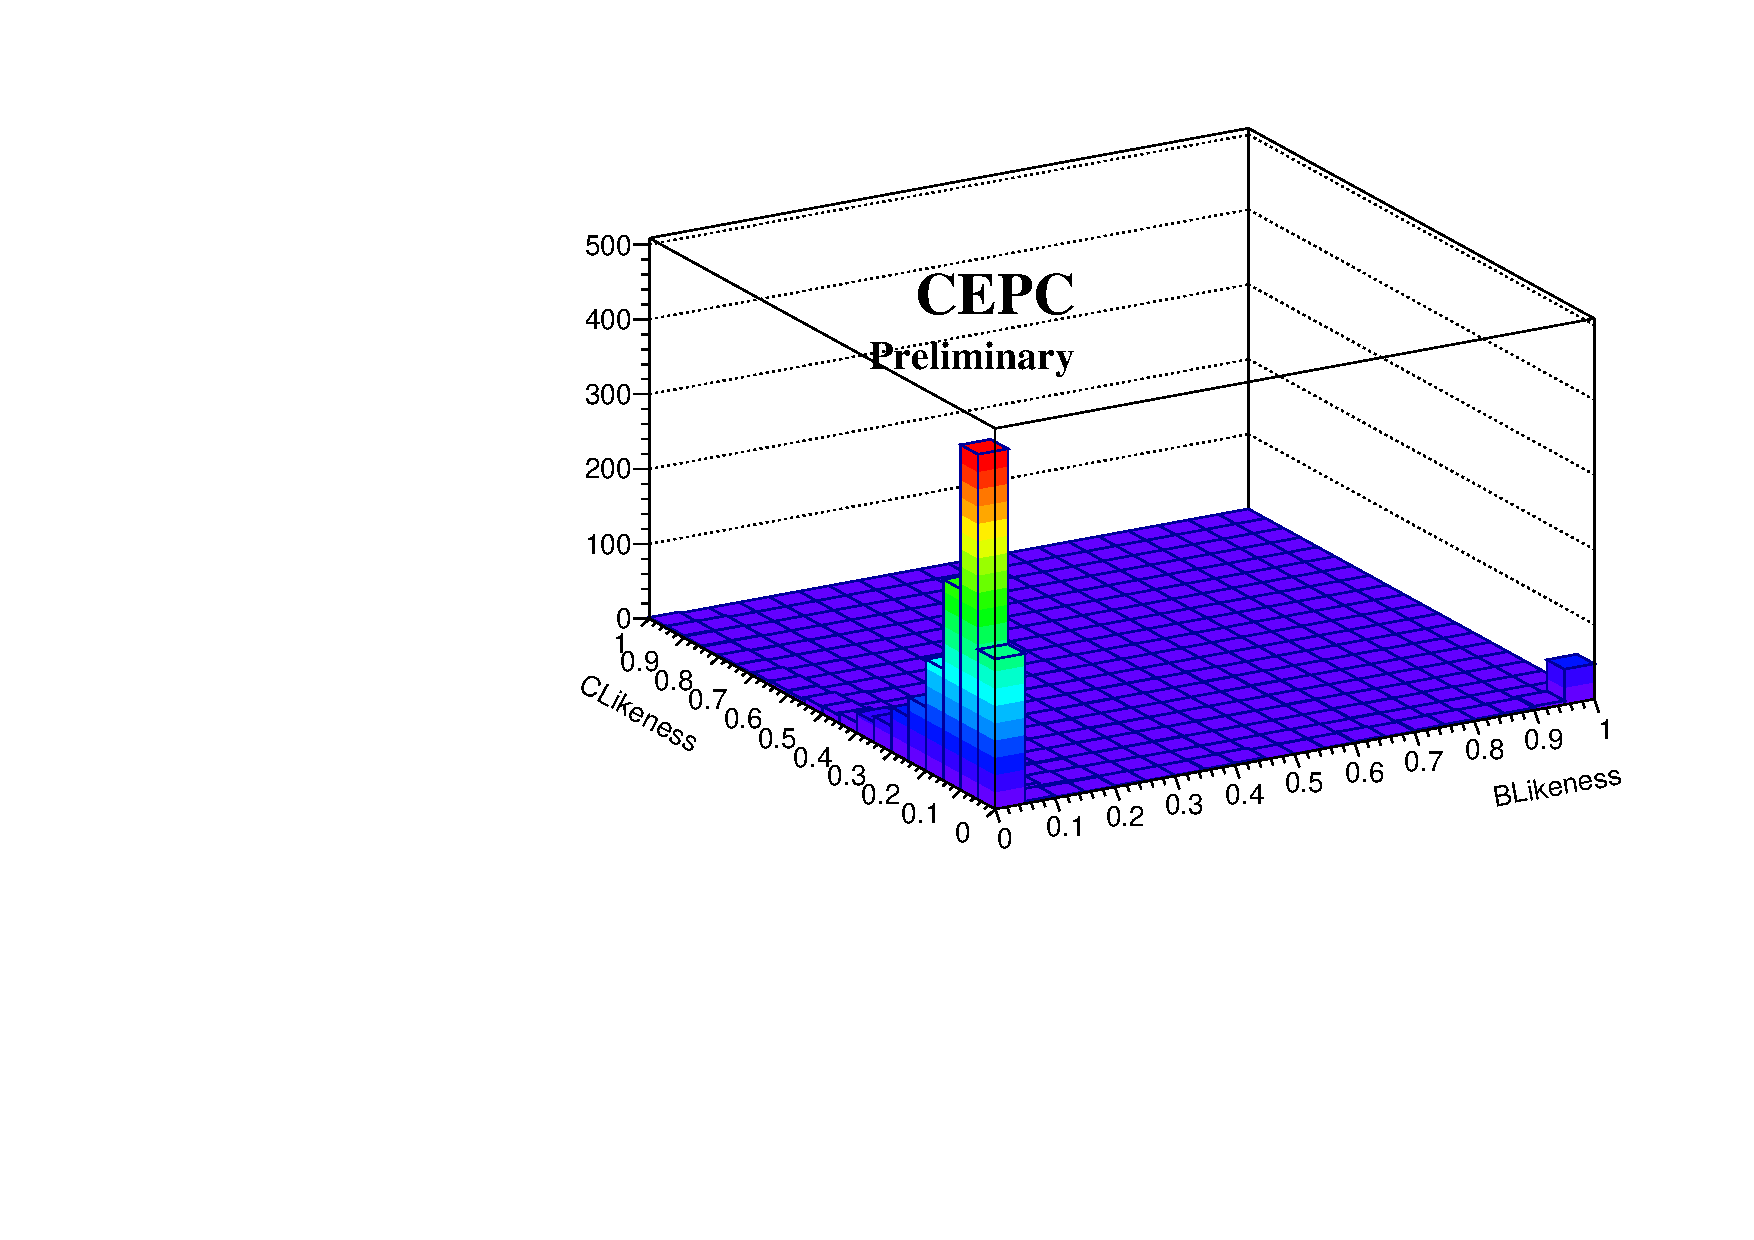
\includegraphics[width=\textwidth]{Template/mumuh_gg.pdf}
    \end{minipage}
}
\subfigure[]
{
    \begin{minipage}[b]{0.31\textwidth}
    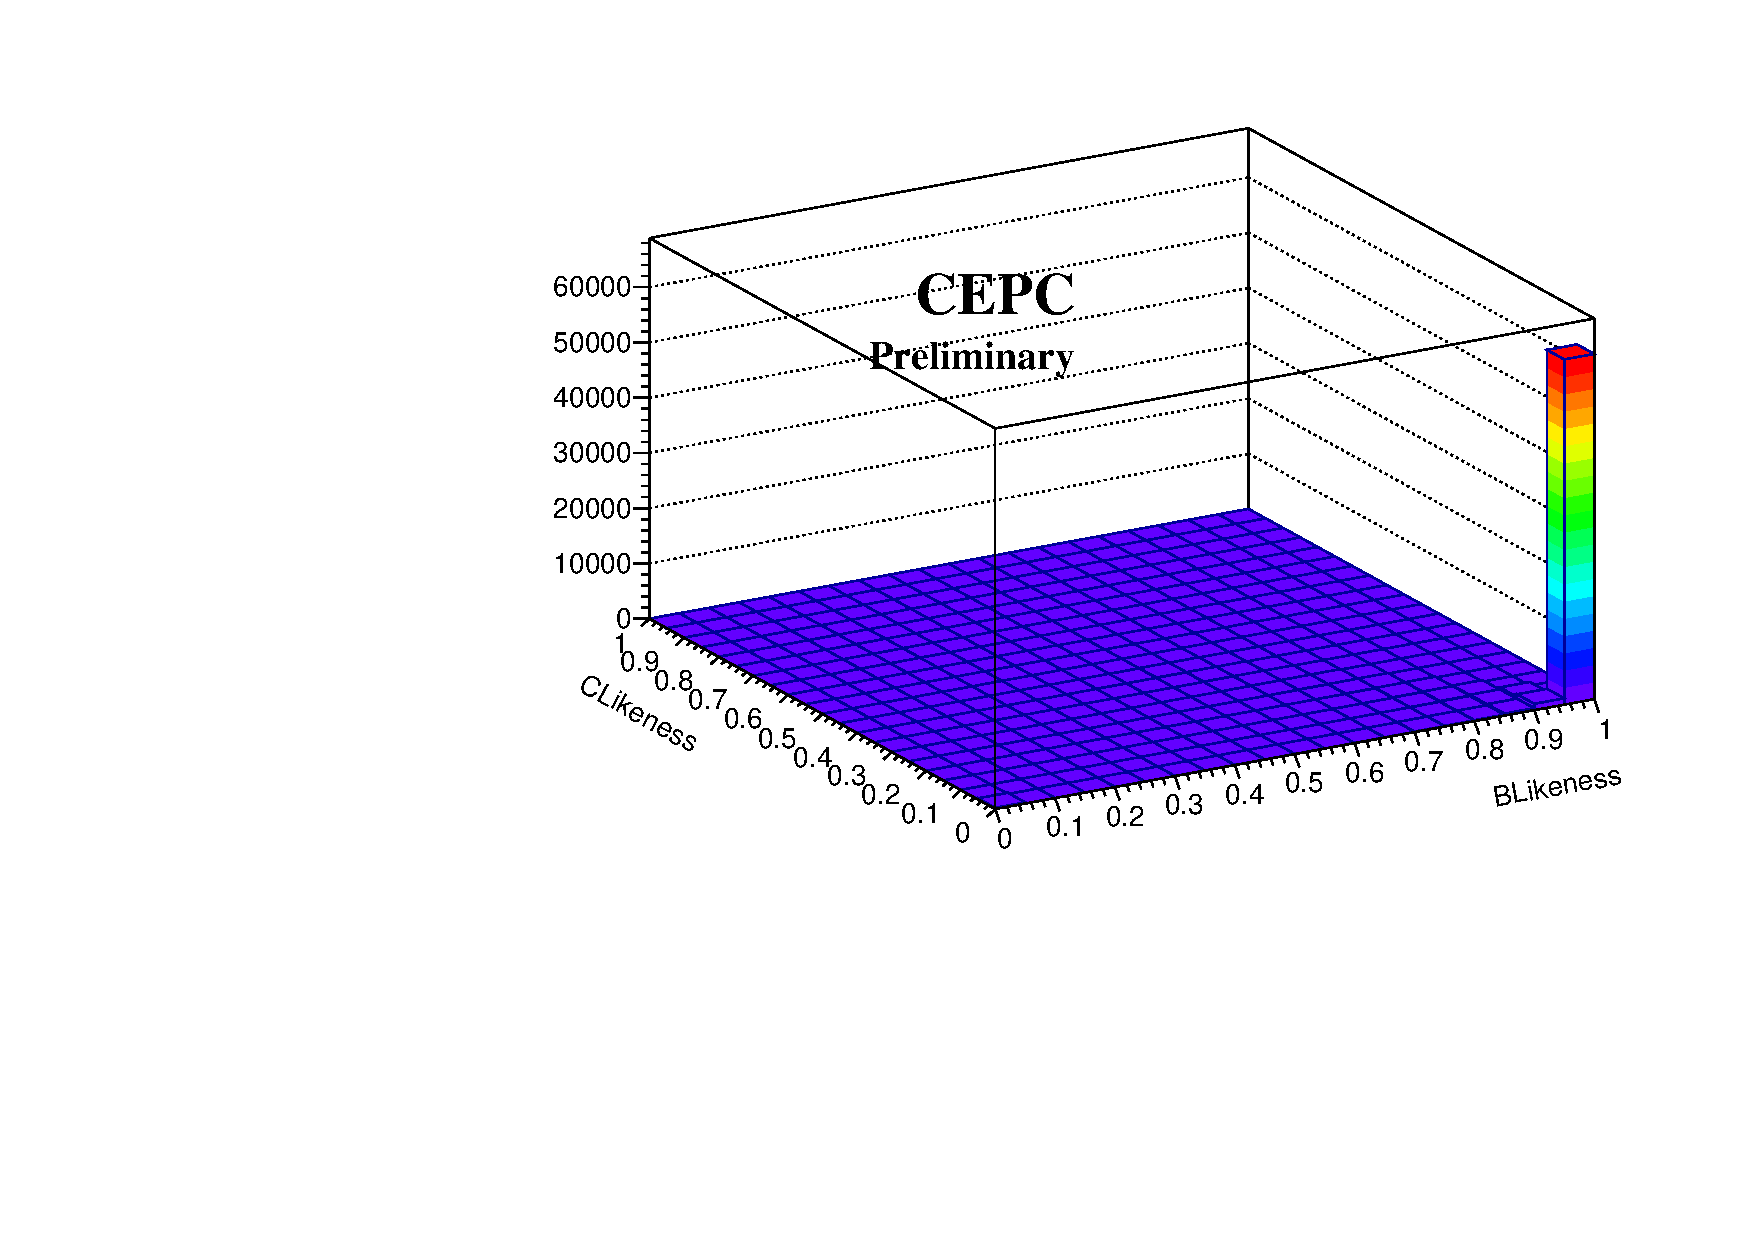
\includegraphics[width=\textwidth]{Template/nnh_bb.pdf}
    \end{minipage}
}
\subfigure[]
{ 
   \begin{minipage}[b]{0.31\textwidth}
   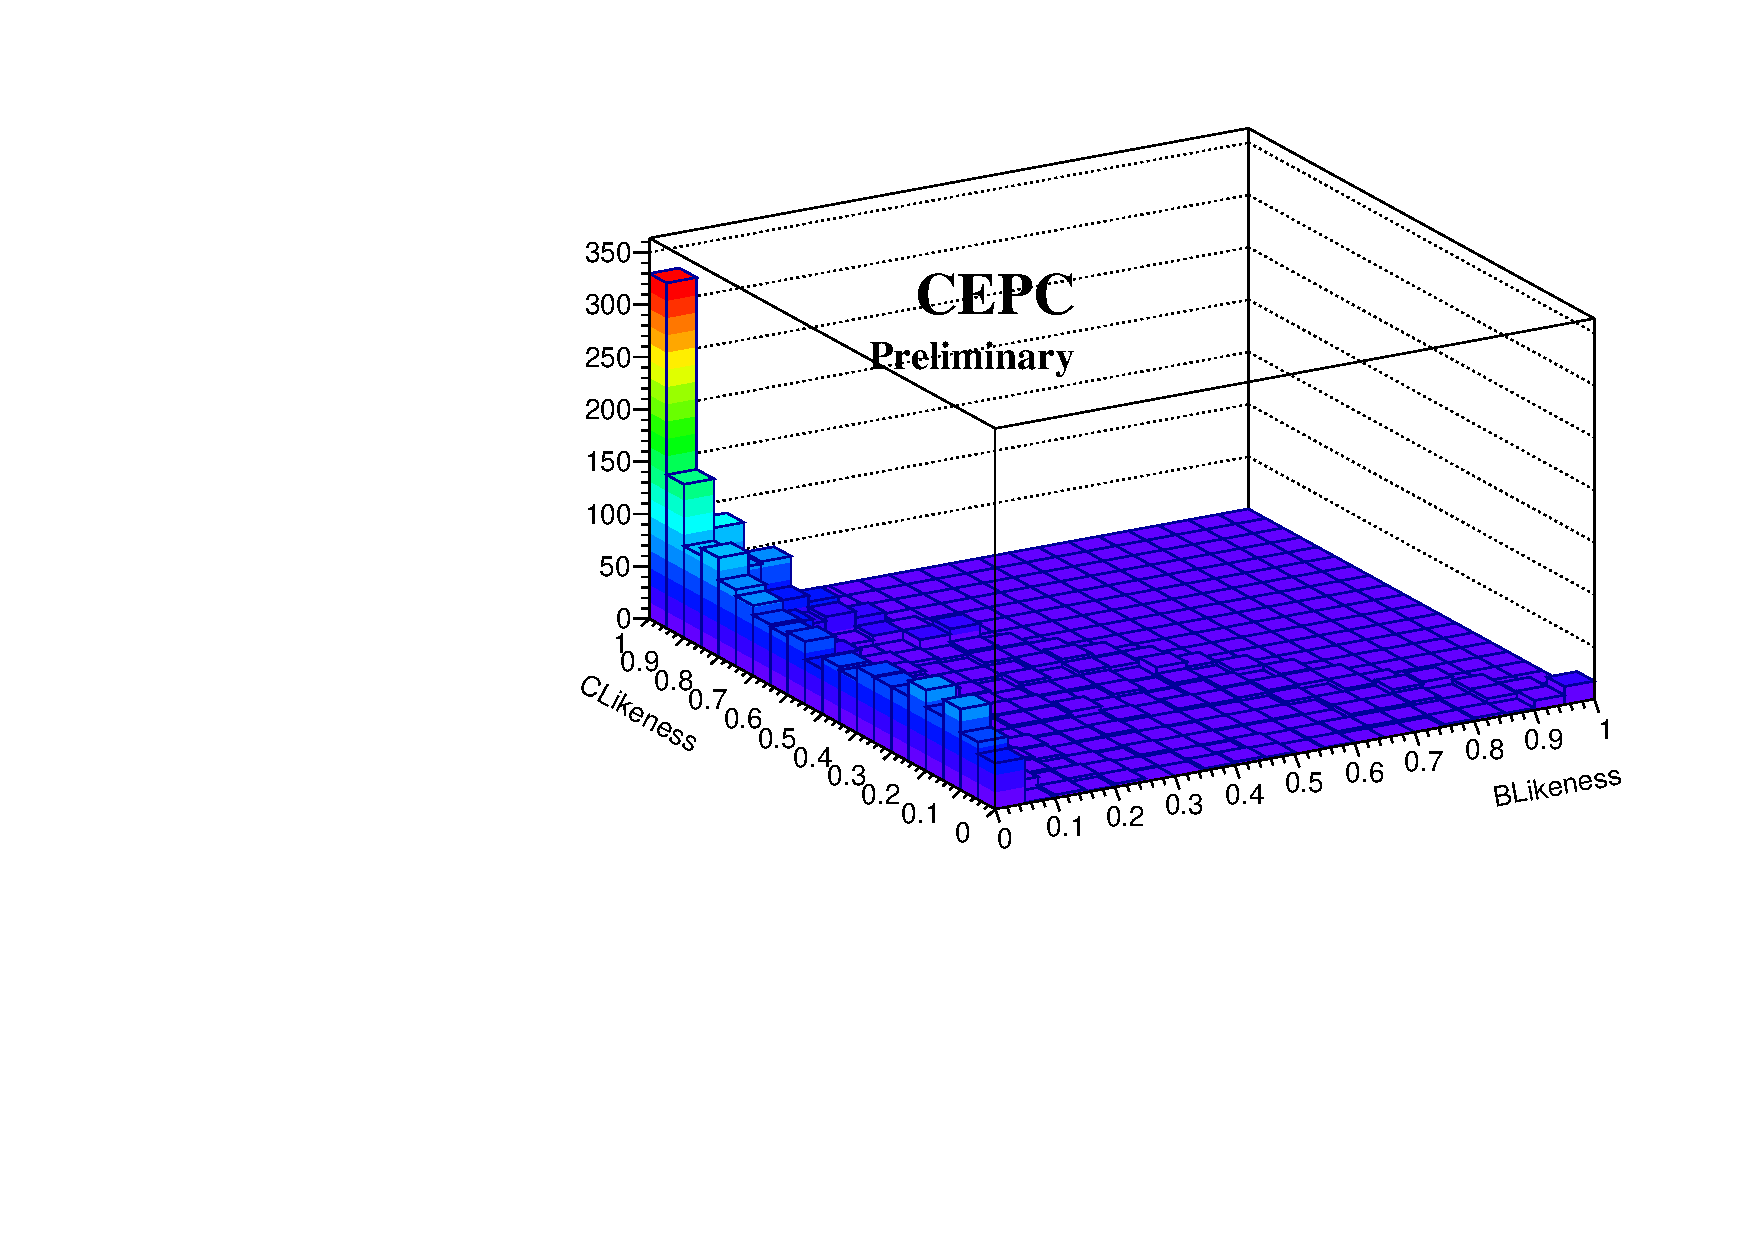
\includegraphics[width=\textwidth]{Template/nnh_cc.pdf}
   \end{minipage}
}
\subfigure[]
{
    \begin{minipage}[b]{0.31\textwidth}
    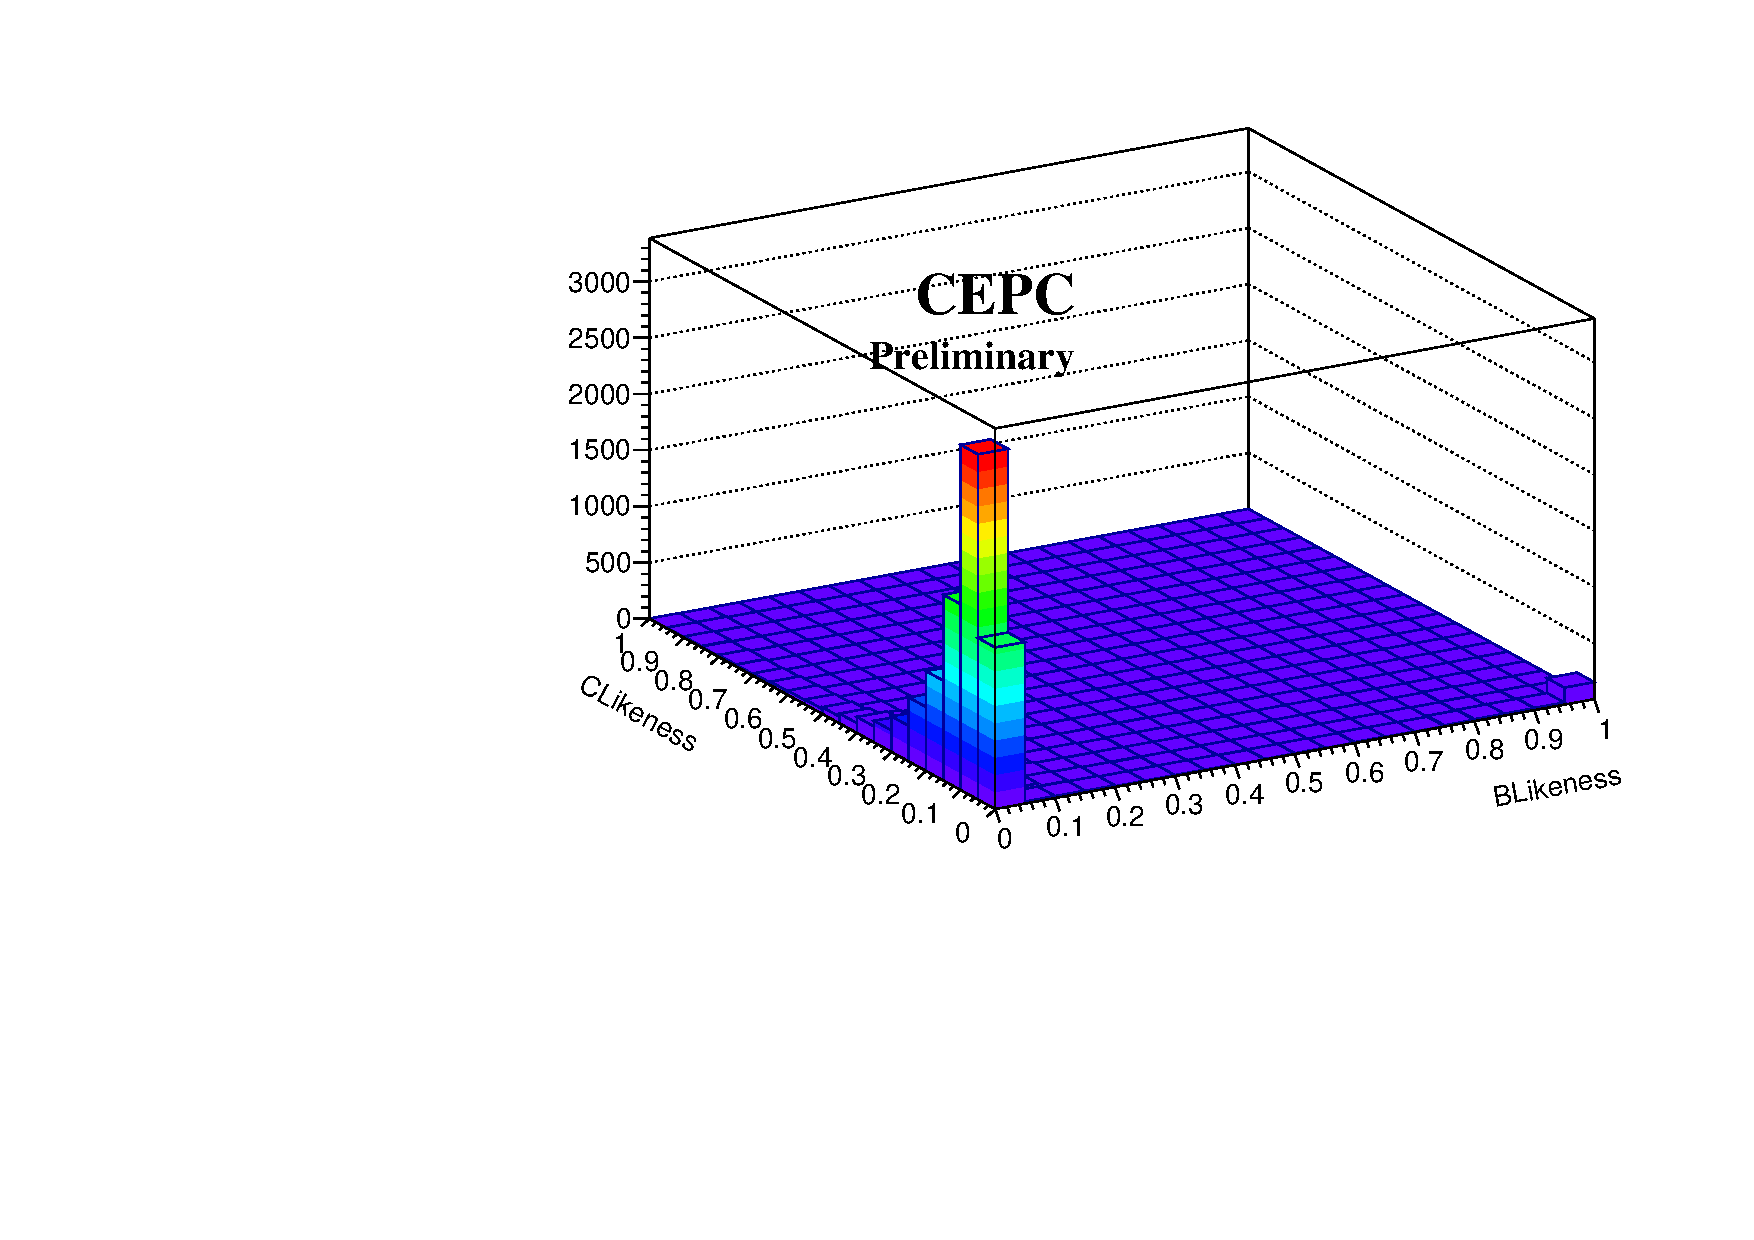
\includegraphics[width=\textwidth]{Template/nnh_gg.pdf}
    \end{minipage}
}
\subfigure[]
{
    \begin{minipage}[b]{0.31\textwidth}
    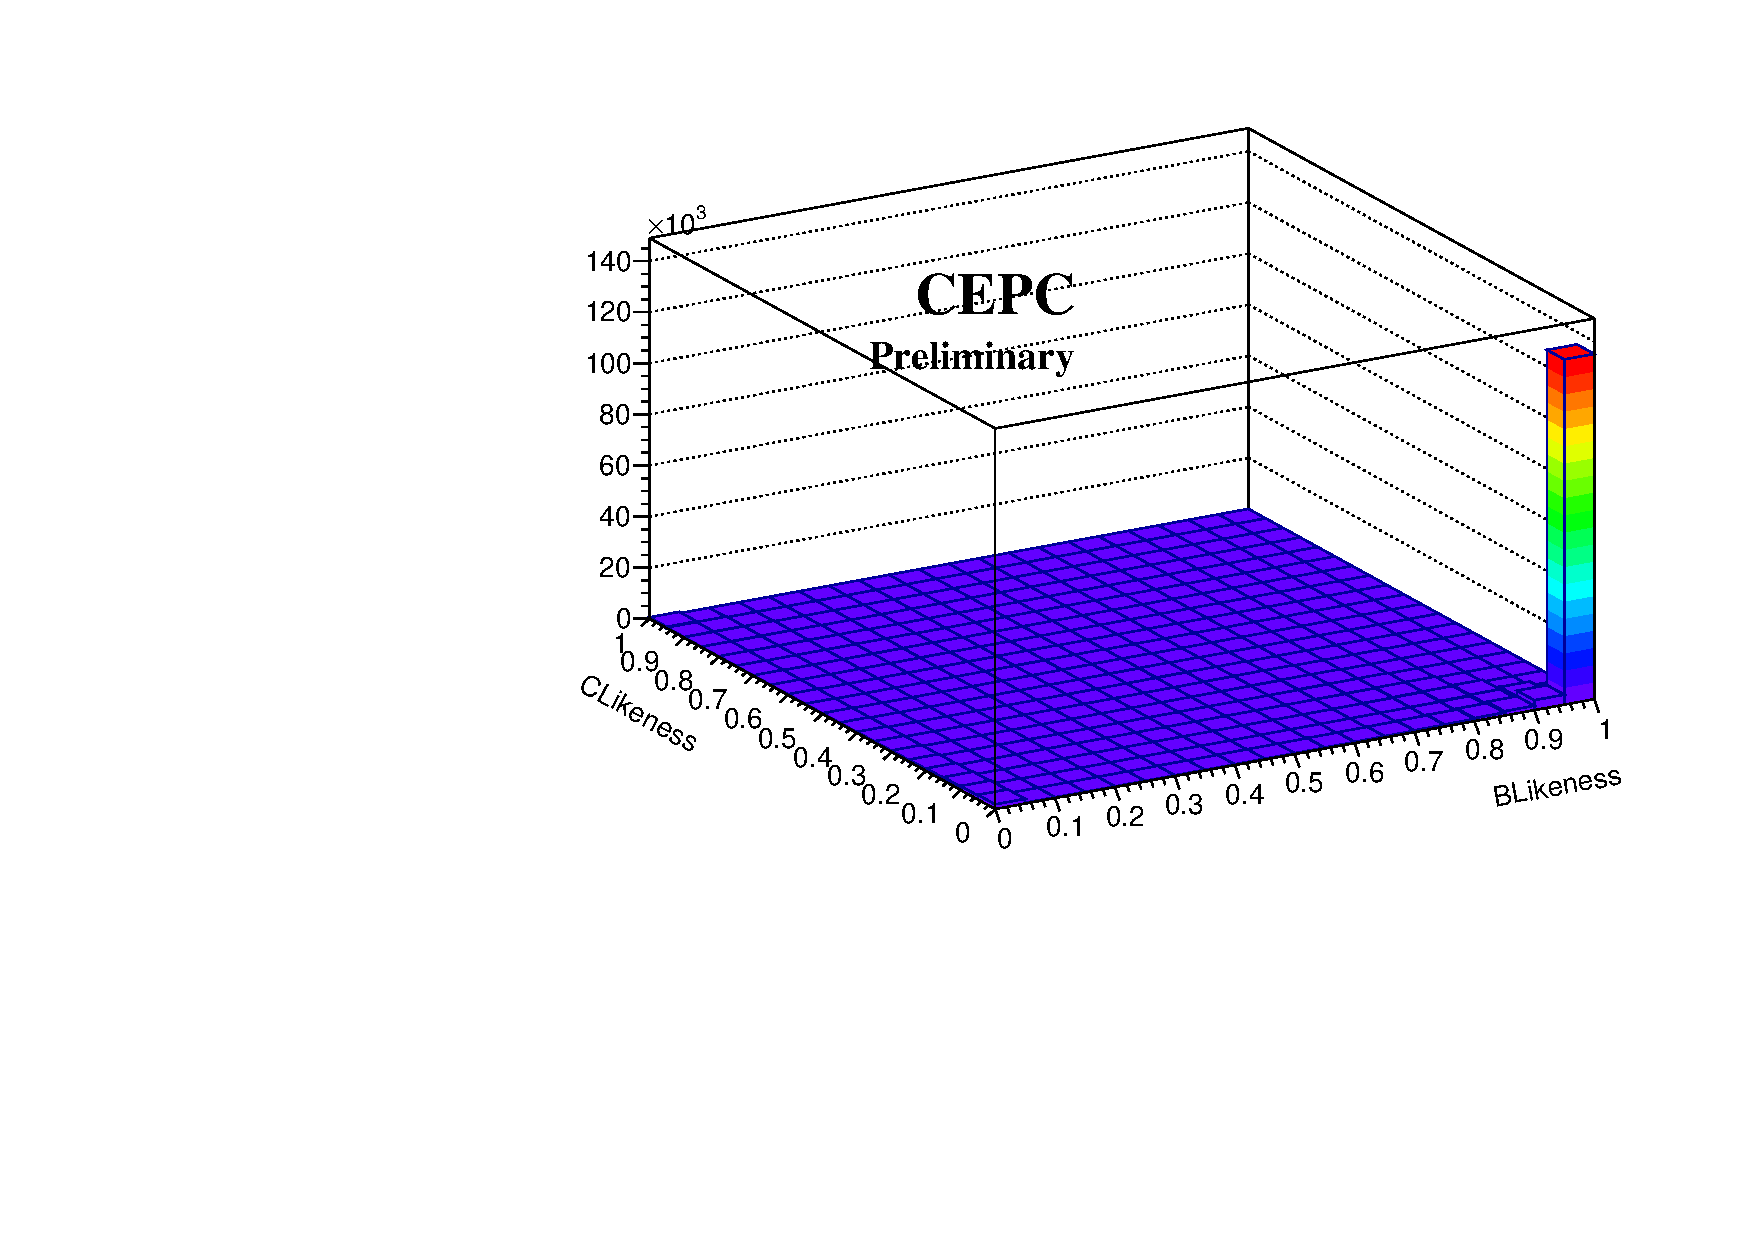
\includegraphics[width=\textwidth]{Template/qqh_bb.pdf}
    \end{minipage}
}
\subfigure[]
{ 
   \begin{minipage}[b]{0.31\textwidth}
   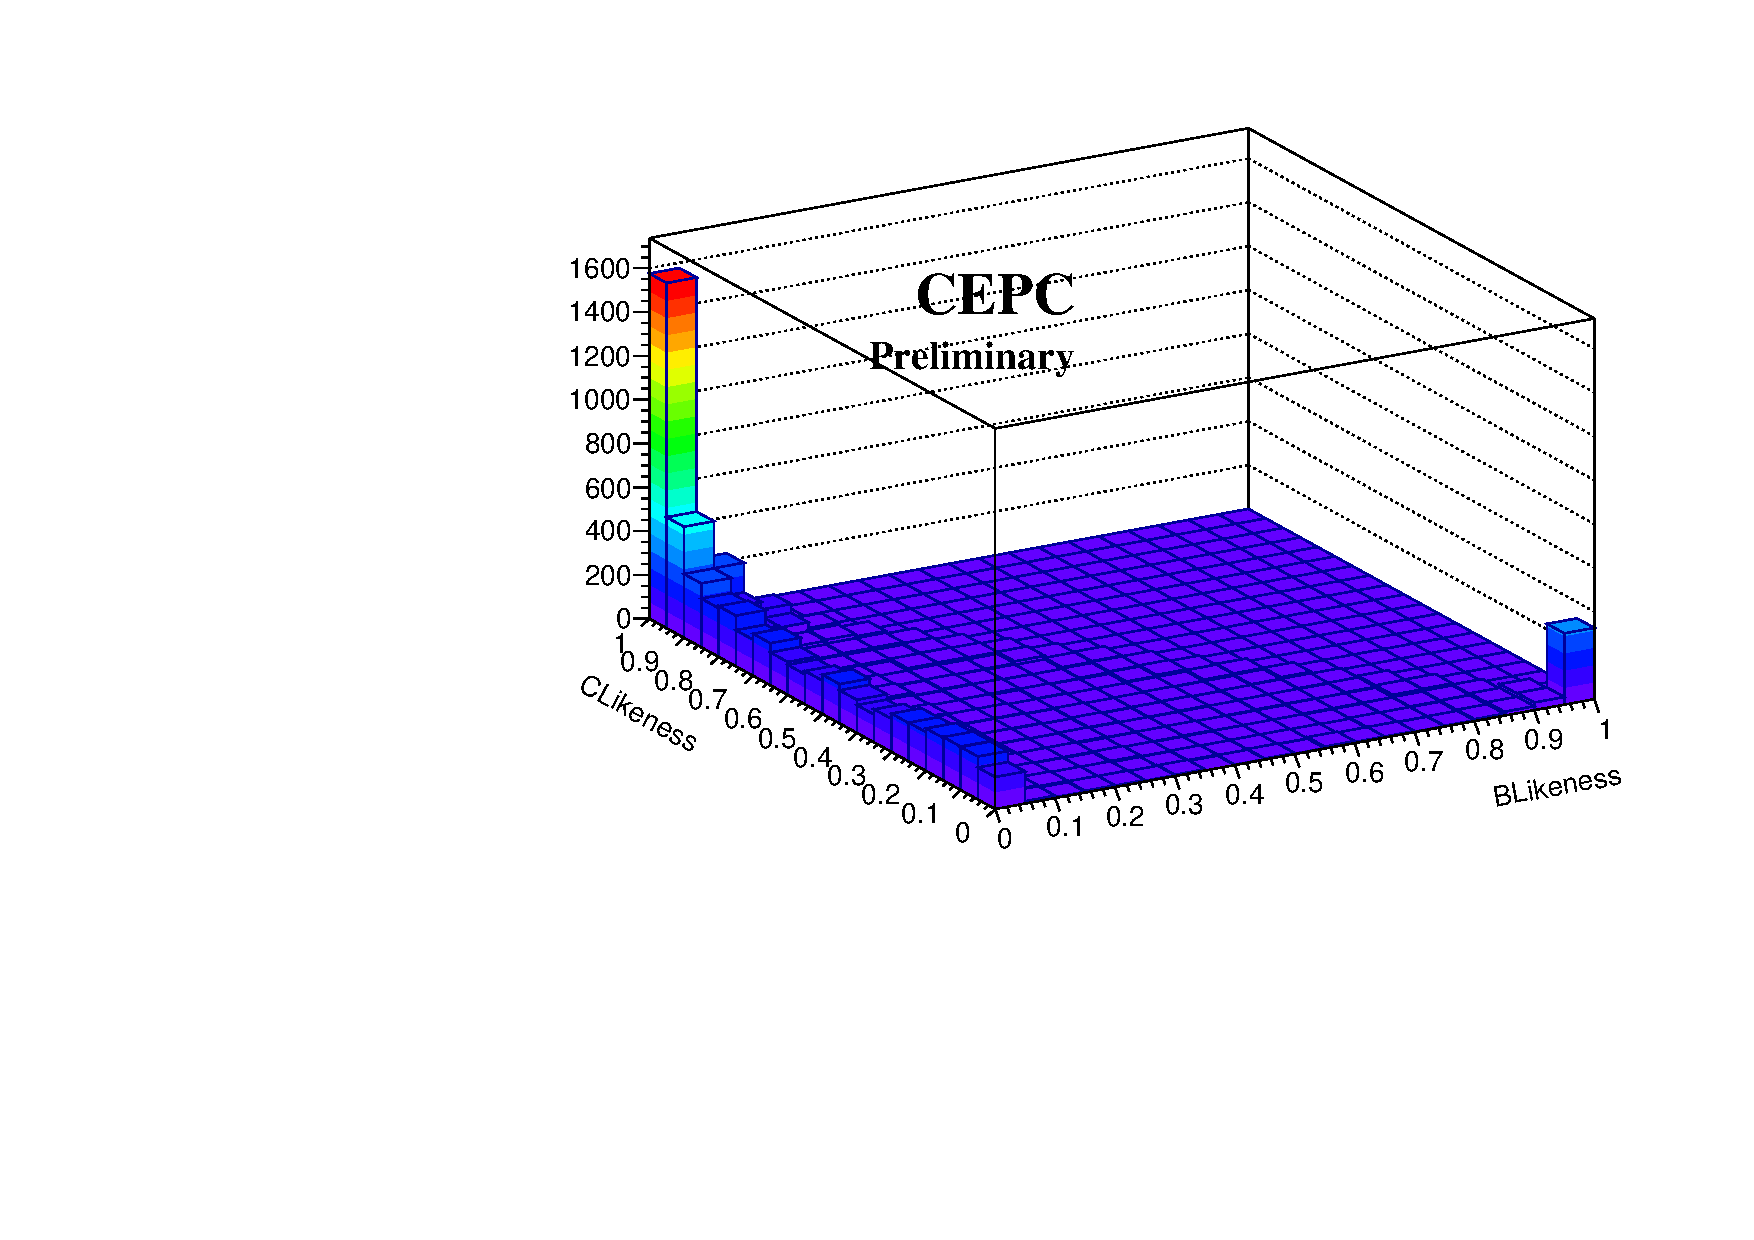
\includegraphics[width=\textwidth]{Template/qqh_cc.pdf}
   \end{minipage}
}
\subfigure[]
{
    \begin{minipage}[b]{0.31\textwidth}
    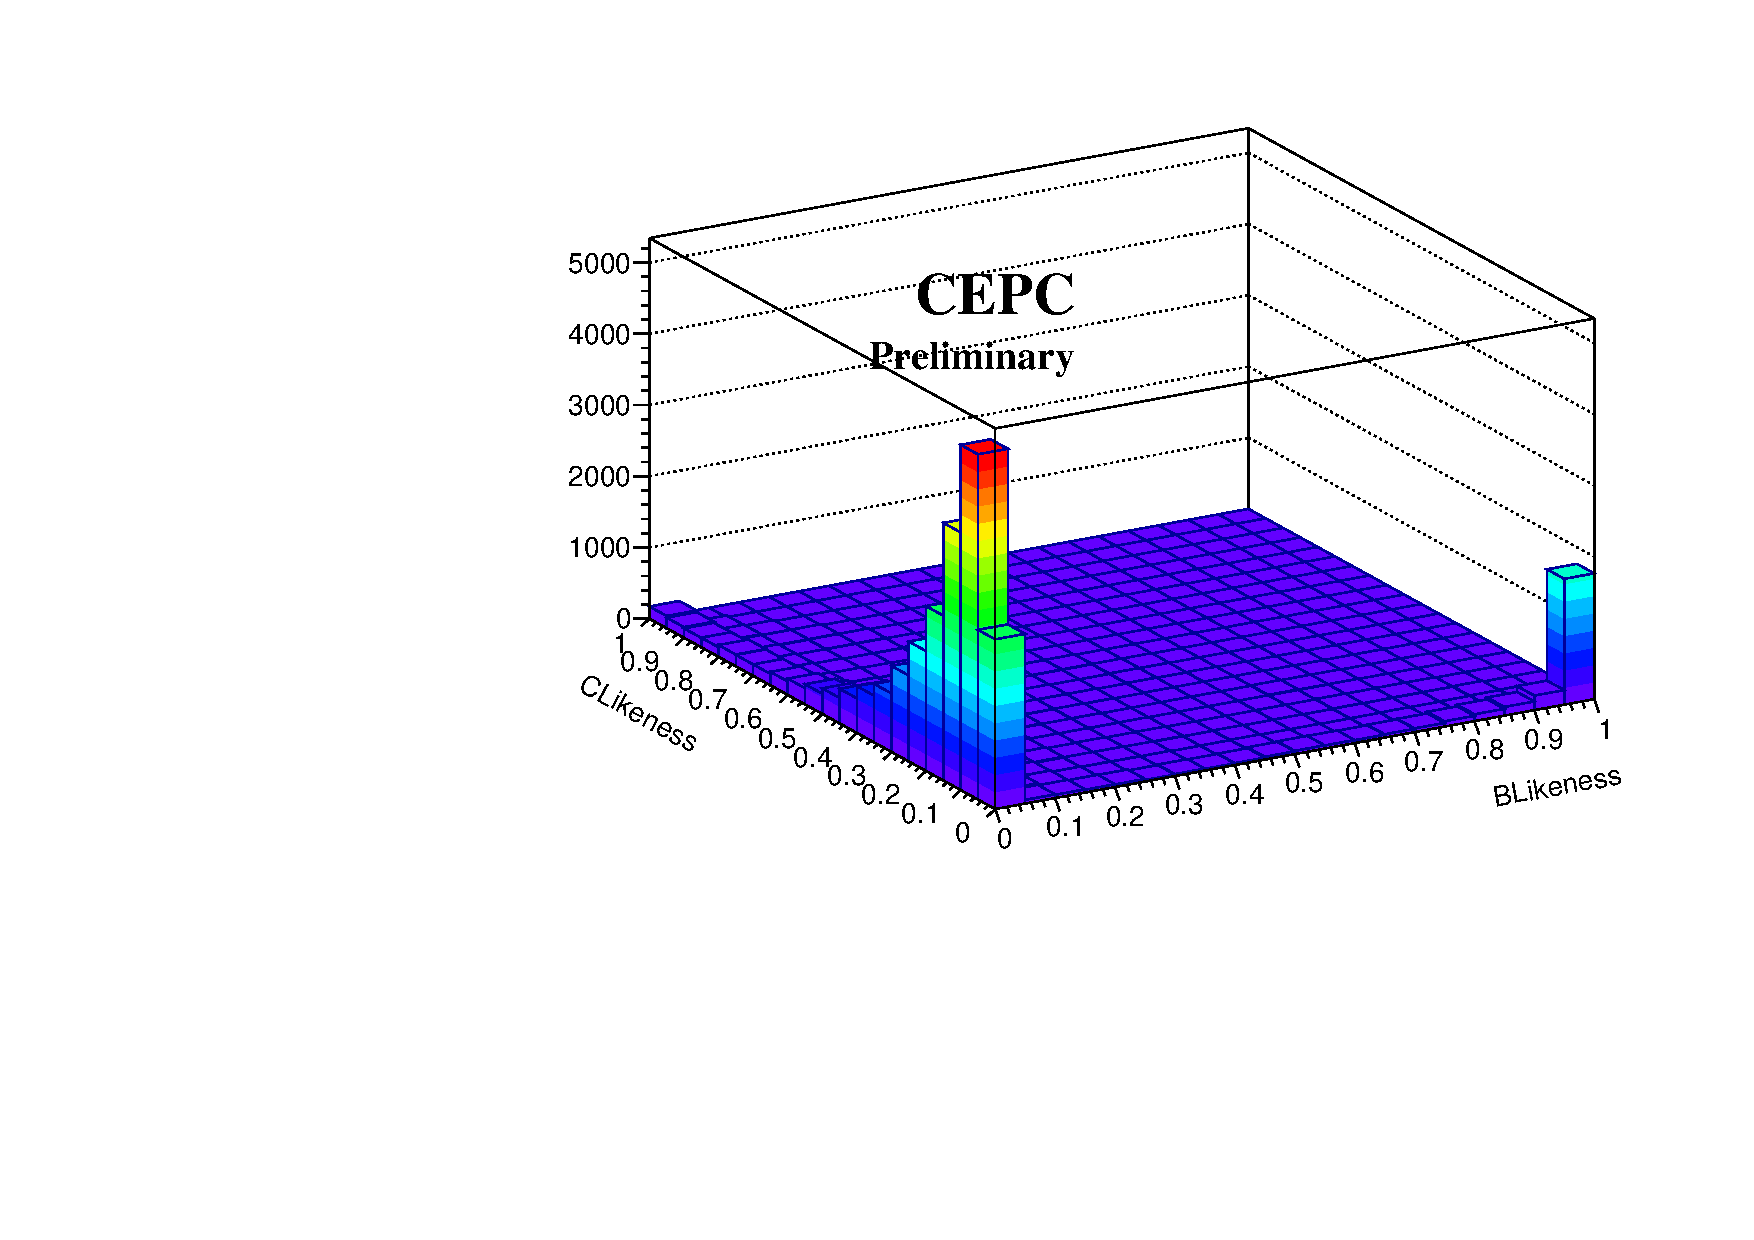
\includegraphics[width=\textwidth]{Template/qqh_gg.pdf}
    \end{minipage}
}
\caption{Template of signal events. From top row to bottom row: templates of \eeh,\mmh,\nnh and \qqh; from left column to right column: templates of $\Hboson\to\bpair$,$\Hboson\to\cpair$ and $\Hboson\to\gpair$.}
\end{figure}

In the fit, the $\Hboson\to\bpair$,$\Hboson\to\cpair$ and $\Hboson\to\gpair$ combined events yield is set as free parameter, which is equal to $L\times \sigma_{ZH\to 4jets}$. The fraction of each of the 3 flavor finals states, say $f_b$,$f_c$ and $f_g$, contribute 2 independent free parameters\footnote{The renormalization requires $f_b+f_c+f_g = 1$, reducing the number of free parameter by 1.}. The shape of backgrounds are fixed. The background distribution was shown in figure \ref{fig:bkg_template}.

\begin{figure}[!htpb]
\label{fig:bkg_template}
\centering
\subfigure[]
{
  \begin{minipage}[b]{0.42\textwidth}
  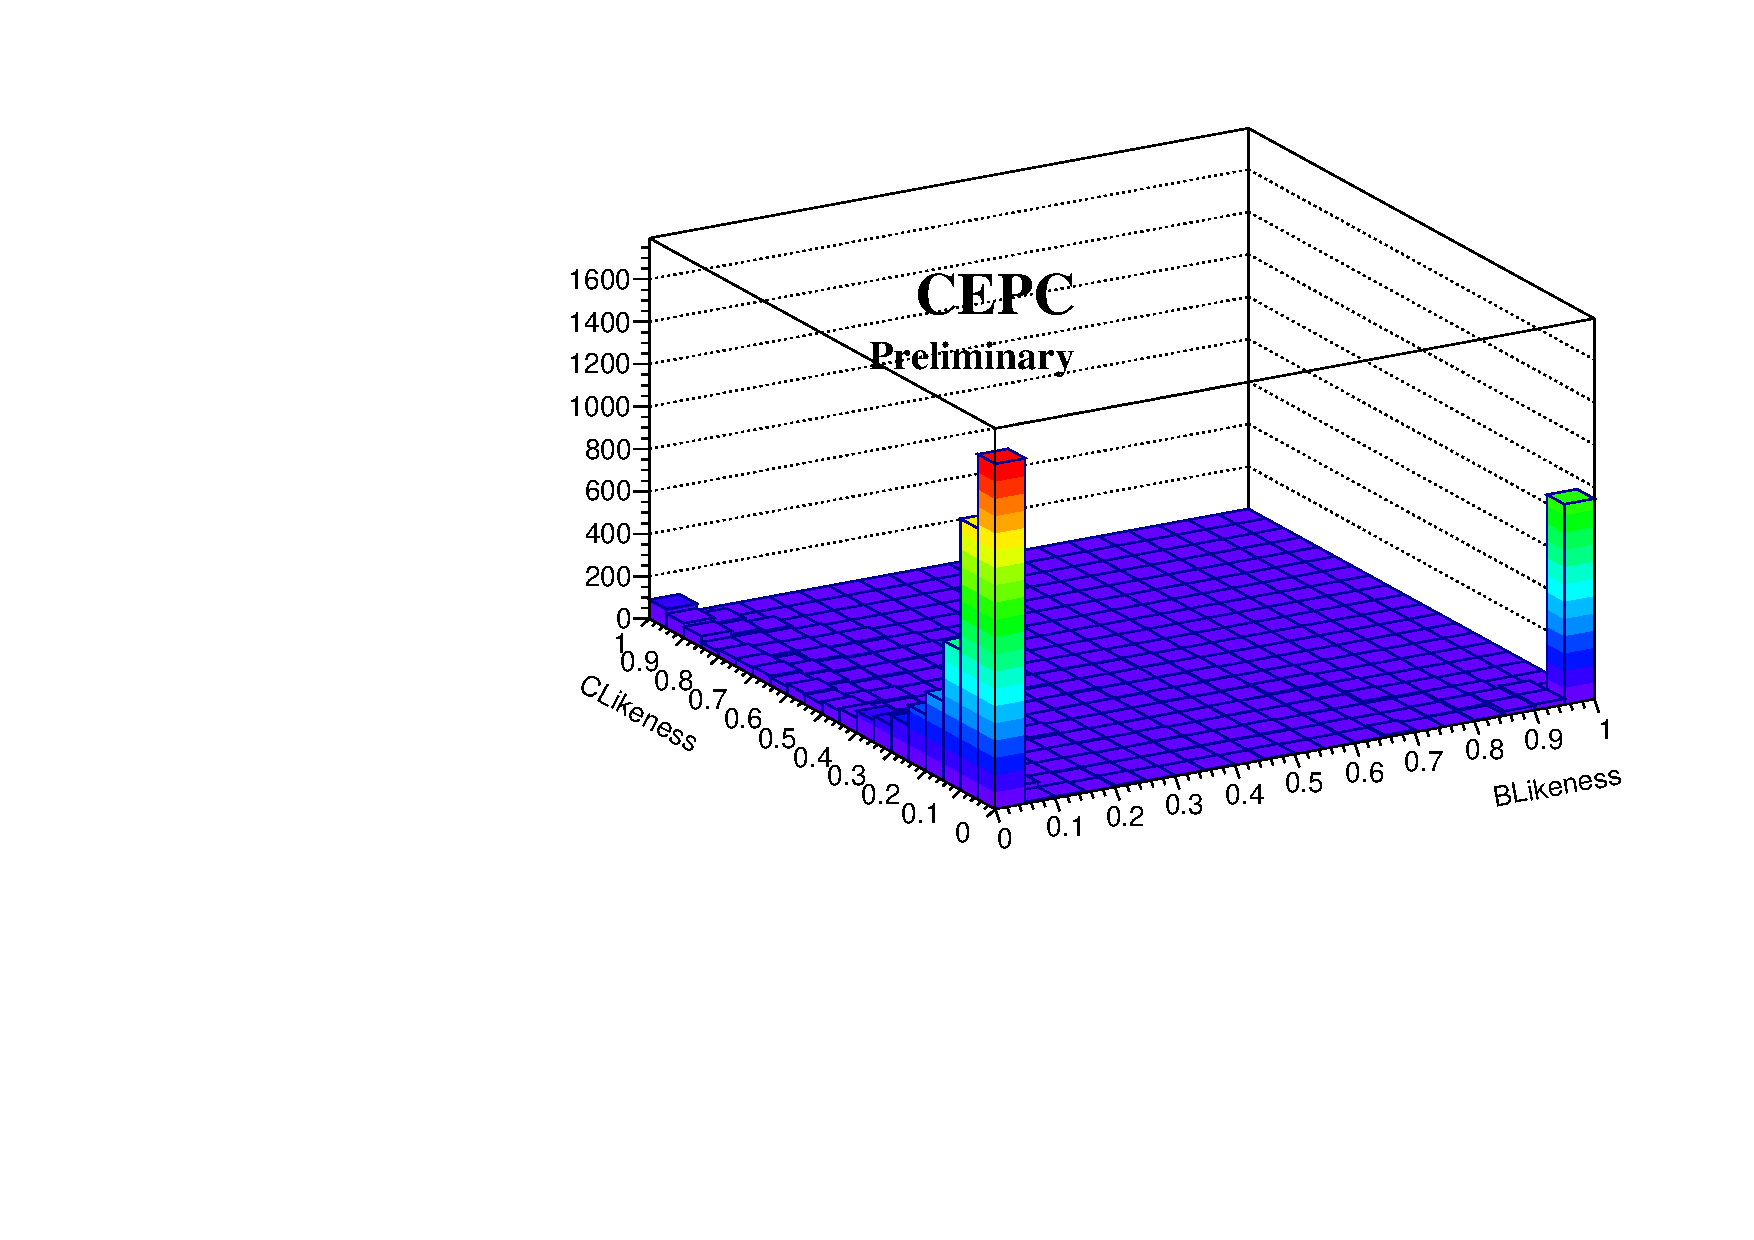
\includegraphics[width=\textwidth]{Template/eeh_bkg.pdf}
  \end{minipage}
}
\subfigure[]
{
  \begin{minipage}[b]{0.42\textwidth}
  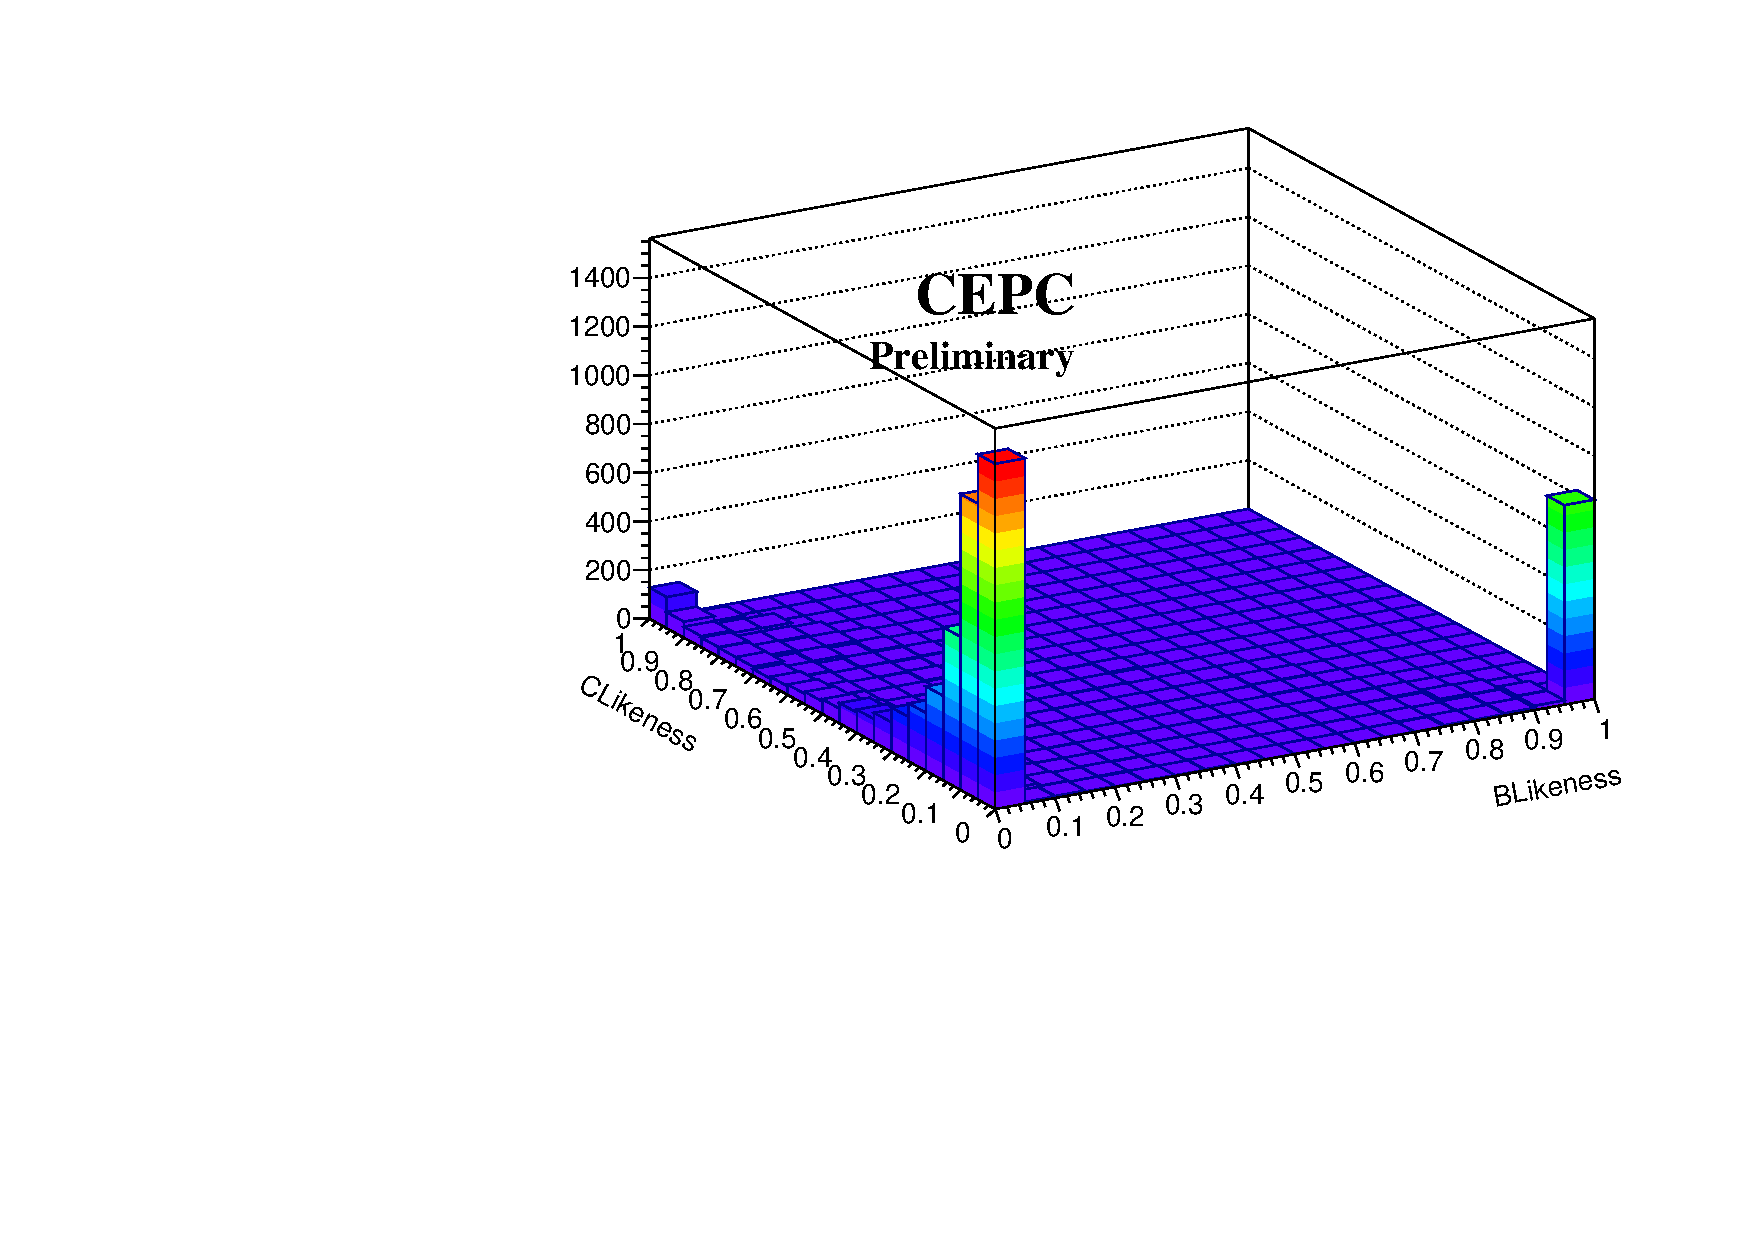
\includegraphics[width=\textwidth]{Template/mumuh_bkg.pdf}
  \end{minipage}
}
\subfigure[]
{ 
   \begin{minipage}[b]{0.42\textwidth}
   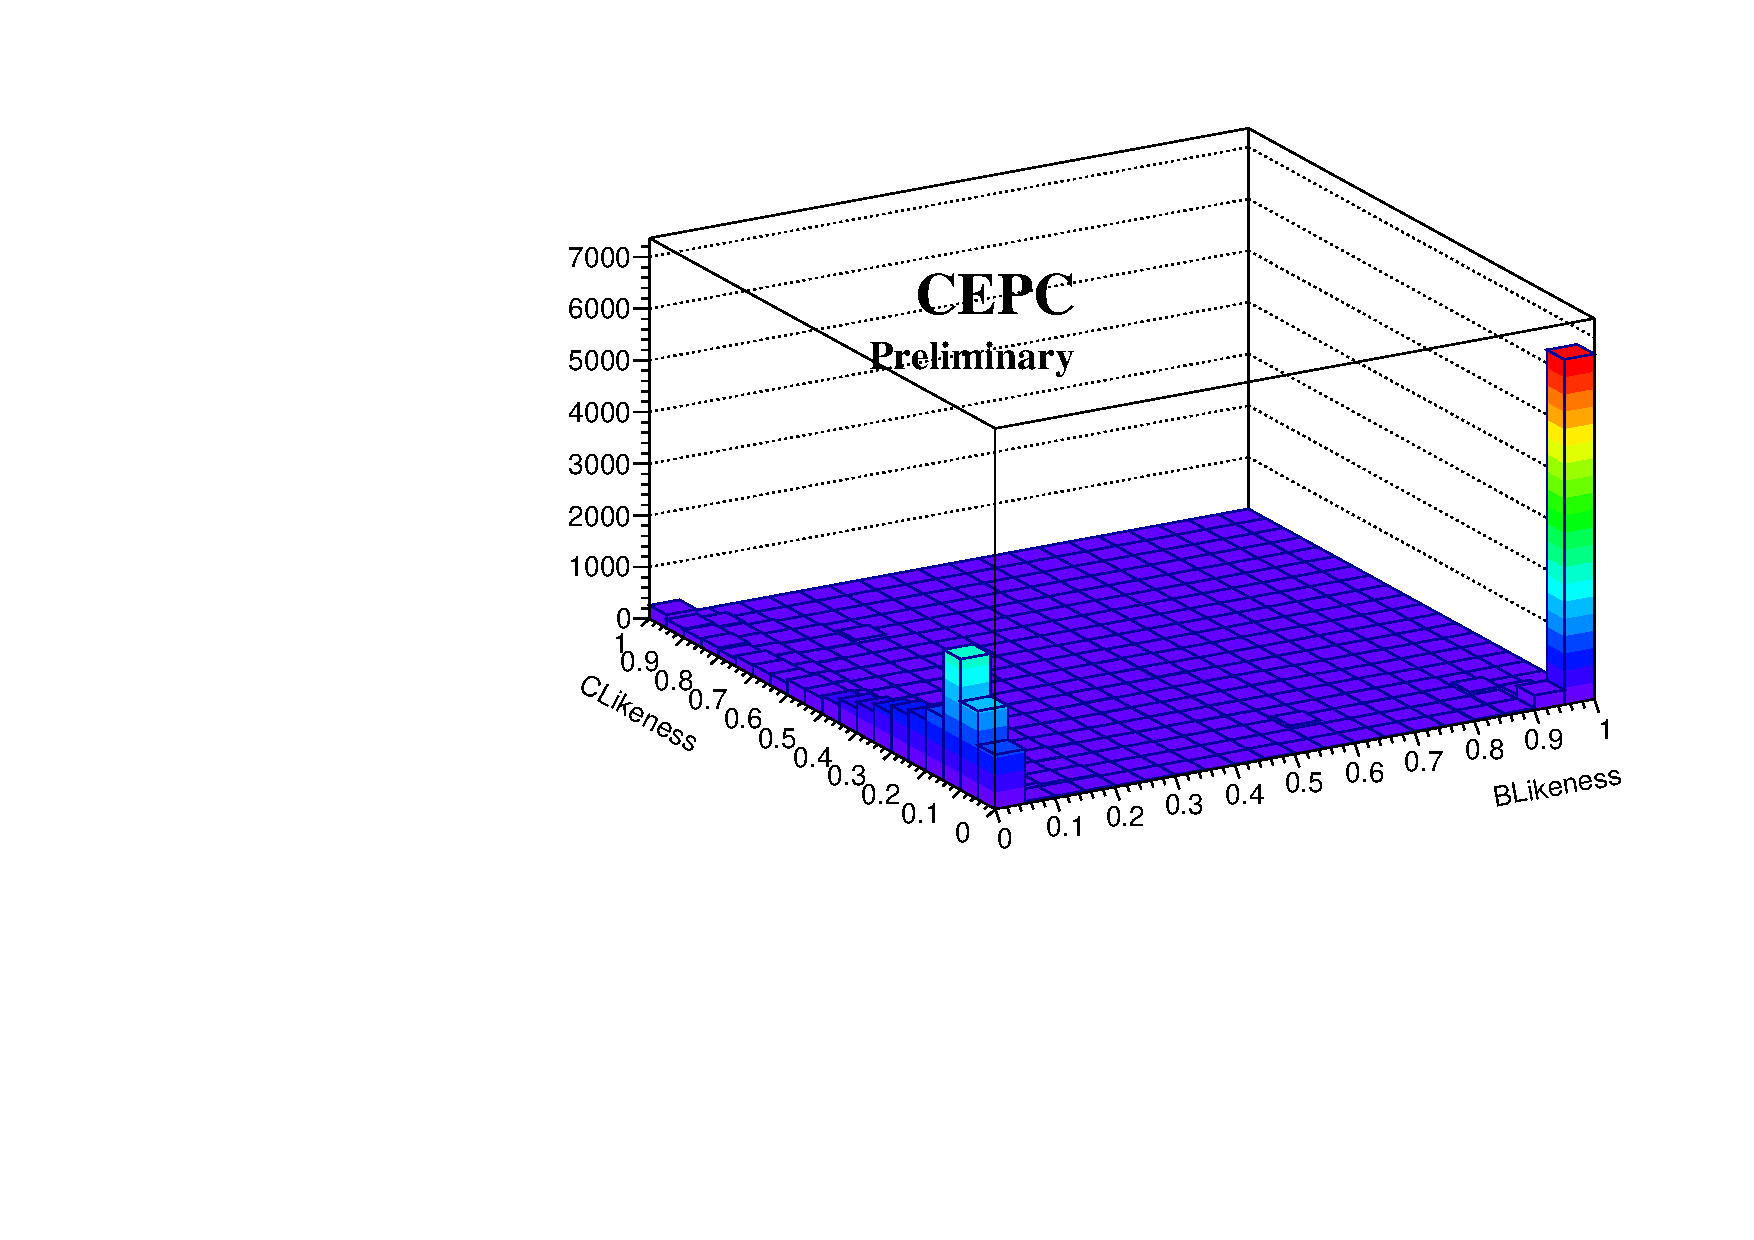
\includegraphics[width=\textwidth]{Template/nnh_bkg.pdf}
   \end{minipage}
}
\subfigure[]
{
    \begin{minipage}[b]{0.42\textwidth}
    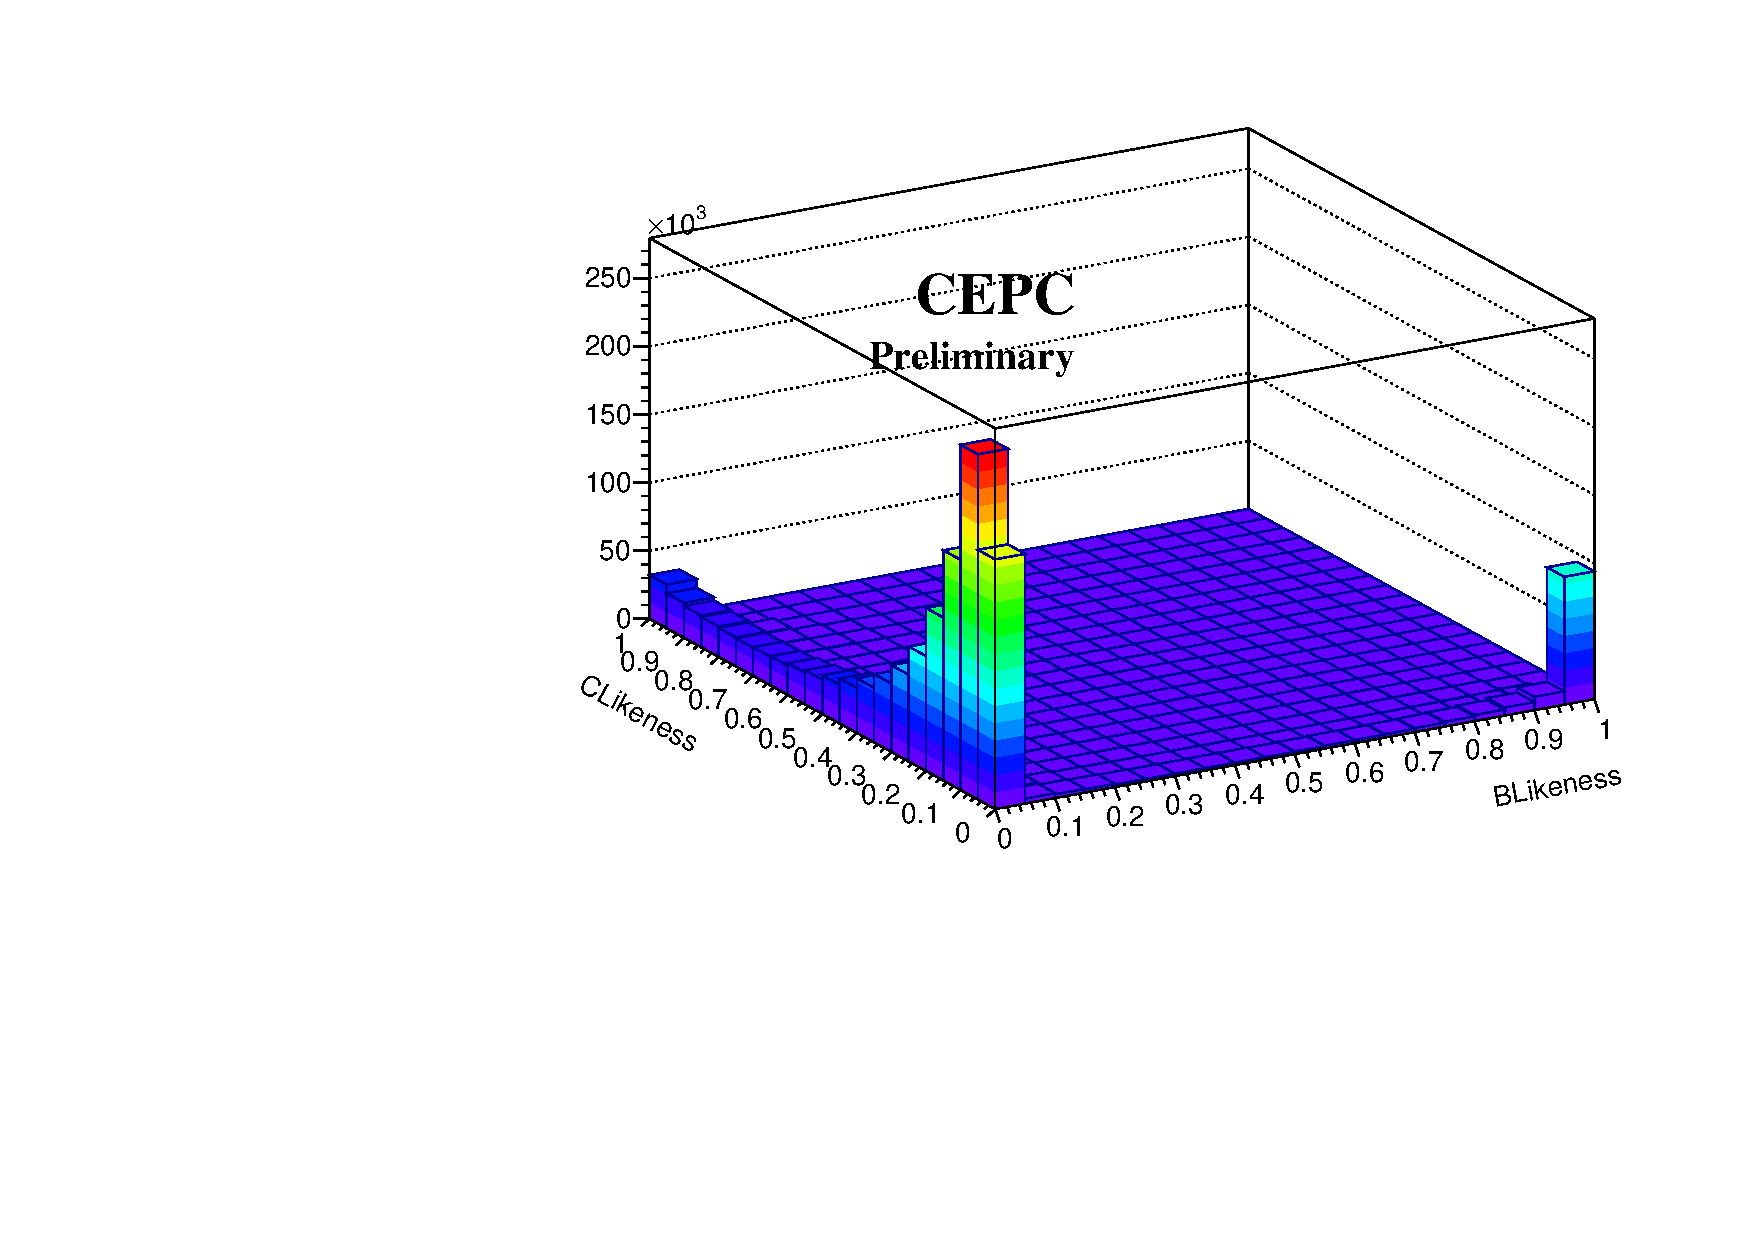
\includegraphics[width=\textwidth]{Template/qqh_bkg.pdf}
    \end{minipage}
}
\caption{Templates of background events in \eeh(top left),\mmh(top right),\nnh(bottom left) and \qqh(bottom right) channel.}
\end{figure}


%\begin{figure}[htpb]
%\centering
%    \includegraphics[width=0.88\textwidth]{figures/c1.eps}
%\caption{ Distribution of $X_B-X_C$ for $H->bb$ (top left), $H->cc$(top right)m $H->gg$ and other $ffH$.
%}
%\label{fig:templates}
%\end{figure}


% To get the jet pair from higgs decay was determined by comparing the $\chi^2$ defined in formula \ref{for:chi2}. With a 21\% possibility to get wrong combination, this is not perfect. The mismatch of PFOs and jets degenerate the paring correct rate. The complication of QCD process and hadronization can significantly affect the correct rate of PFO jet matching:
% \begin{itemize}
% \item Gluon radiation: give rise to considerable charge in partons momentum.  
% \item Gluon splitting: causing a more complex final states with additional parton
% \end{itemize}


\subsection{ToyMC test with templatefit}
A ToyMC test was applied to evaluate the uncertainty from template fit. In this test, the template fit was done repeatly to the different datasets, in which events yields at each bin on the $X_B-X_C$ distribution are set to be random value according to Possion distribution. This test deomonstrate the unceratiny from the fit  due to data statistic fluctuation. The fit results for $\eeh$, $\mmh$, $\nnh$ and $\qqh$ are shown in figure \ref{fig:toymc_subchannel}. 

\begin{figure}[!htpb]
\centering
\subfigure[]
{
     \begin{minipage}[b]{0.31\textwidth}
     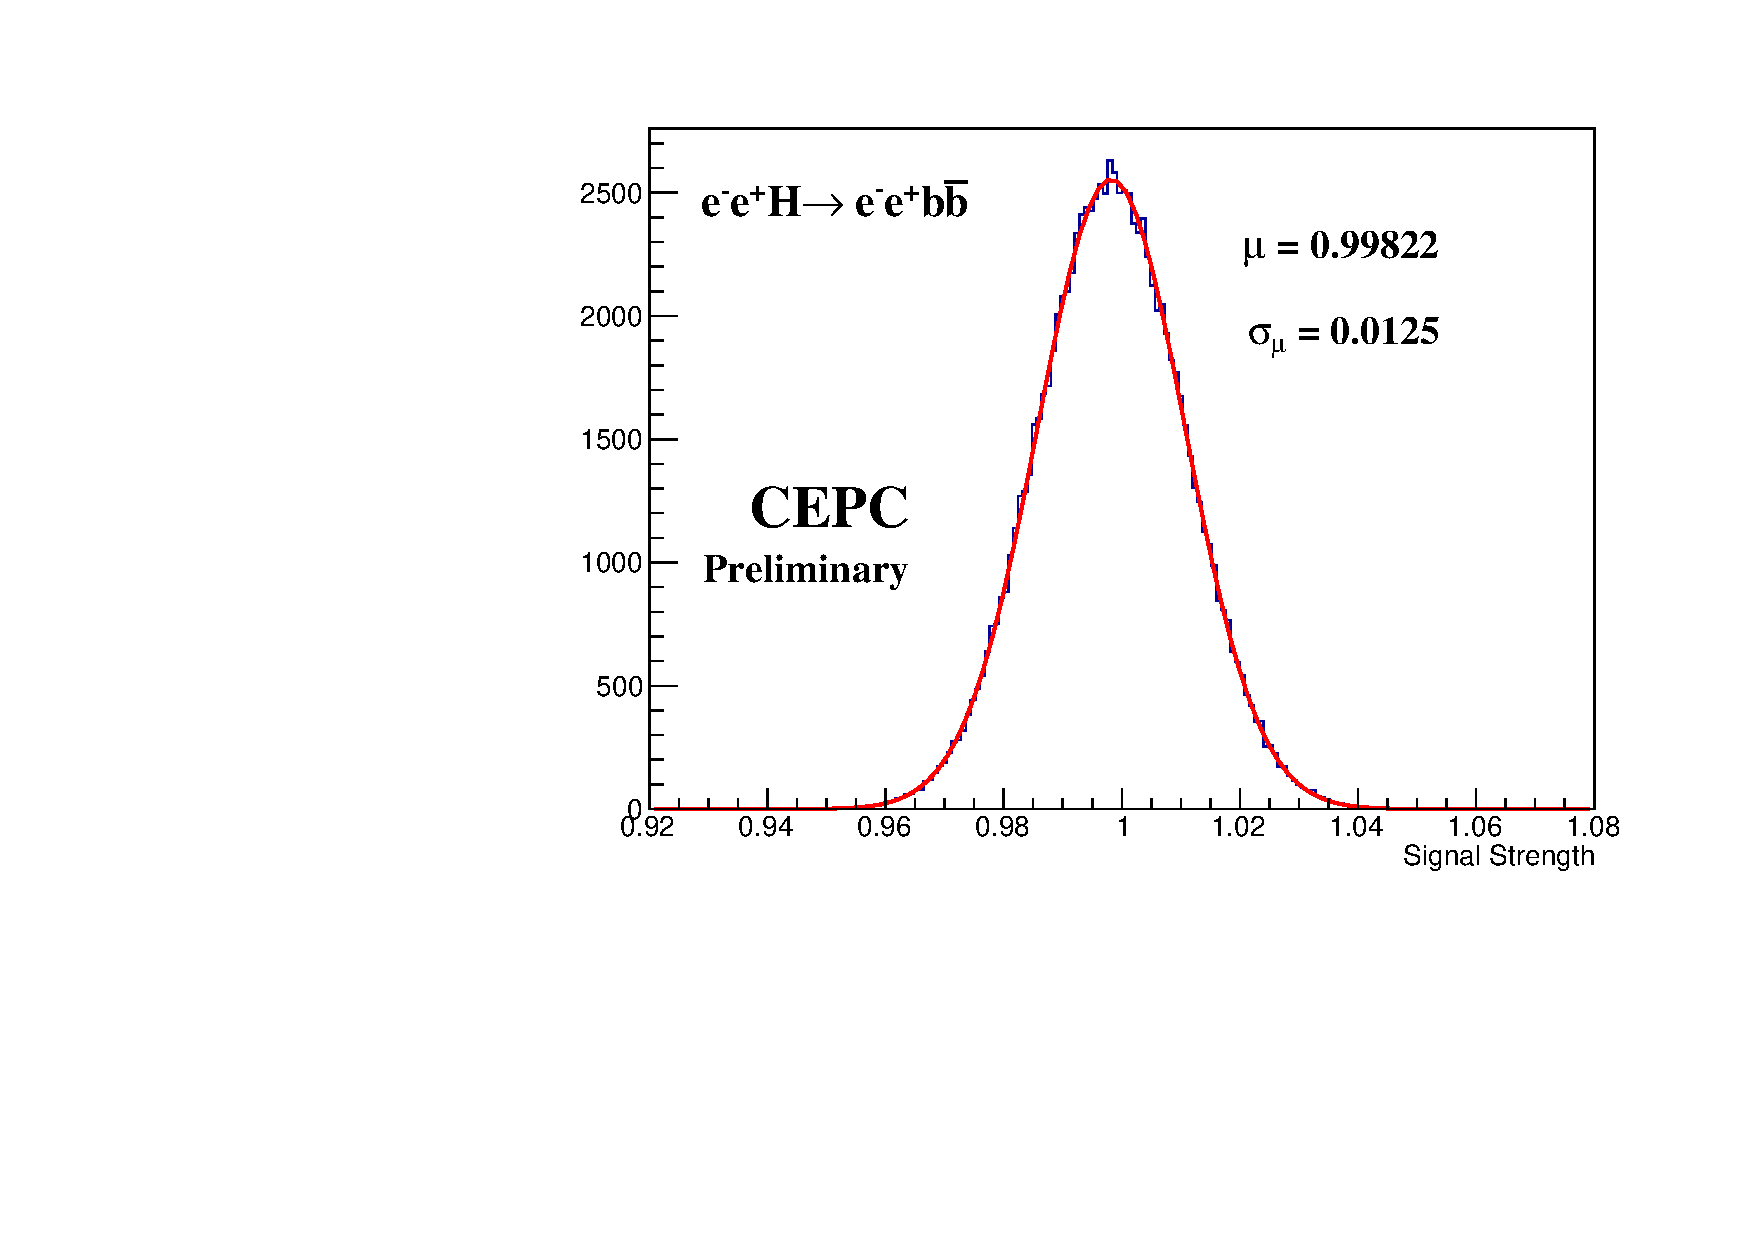
\includegraphics[width=\textwidth]{Template/toymc_eeh_bb.pdf}
     \end{minipage}
}
\subfigure[]
{
     \begin{minipage}[b]{0.31\textwidth}
     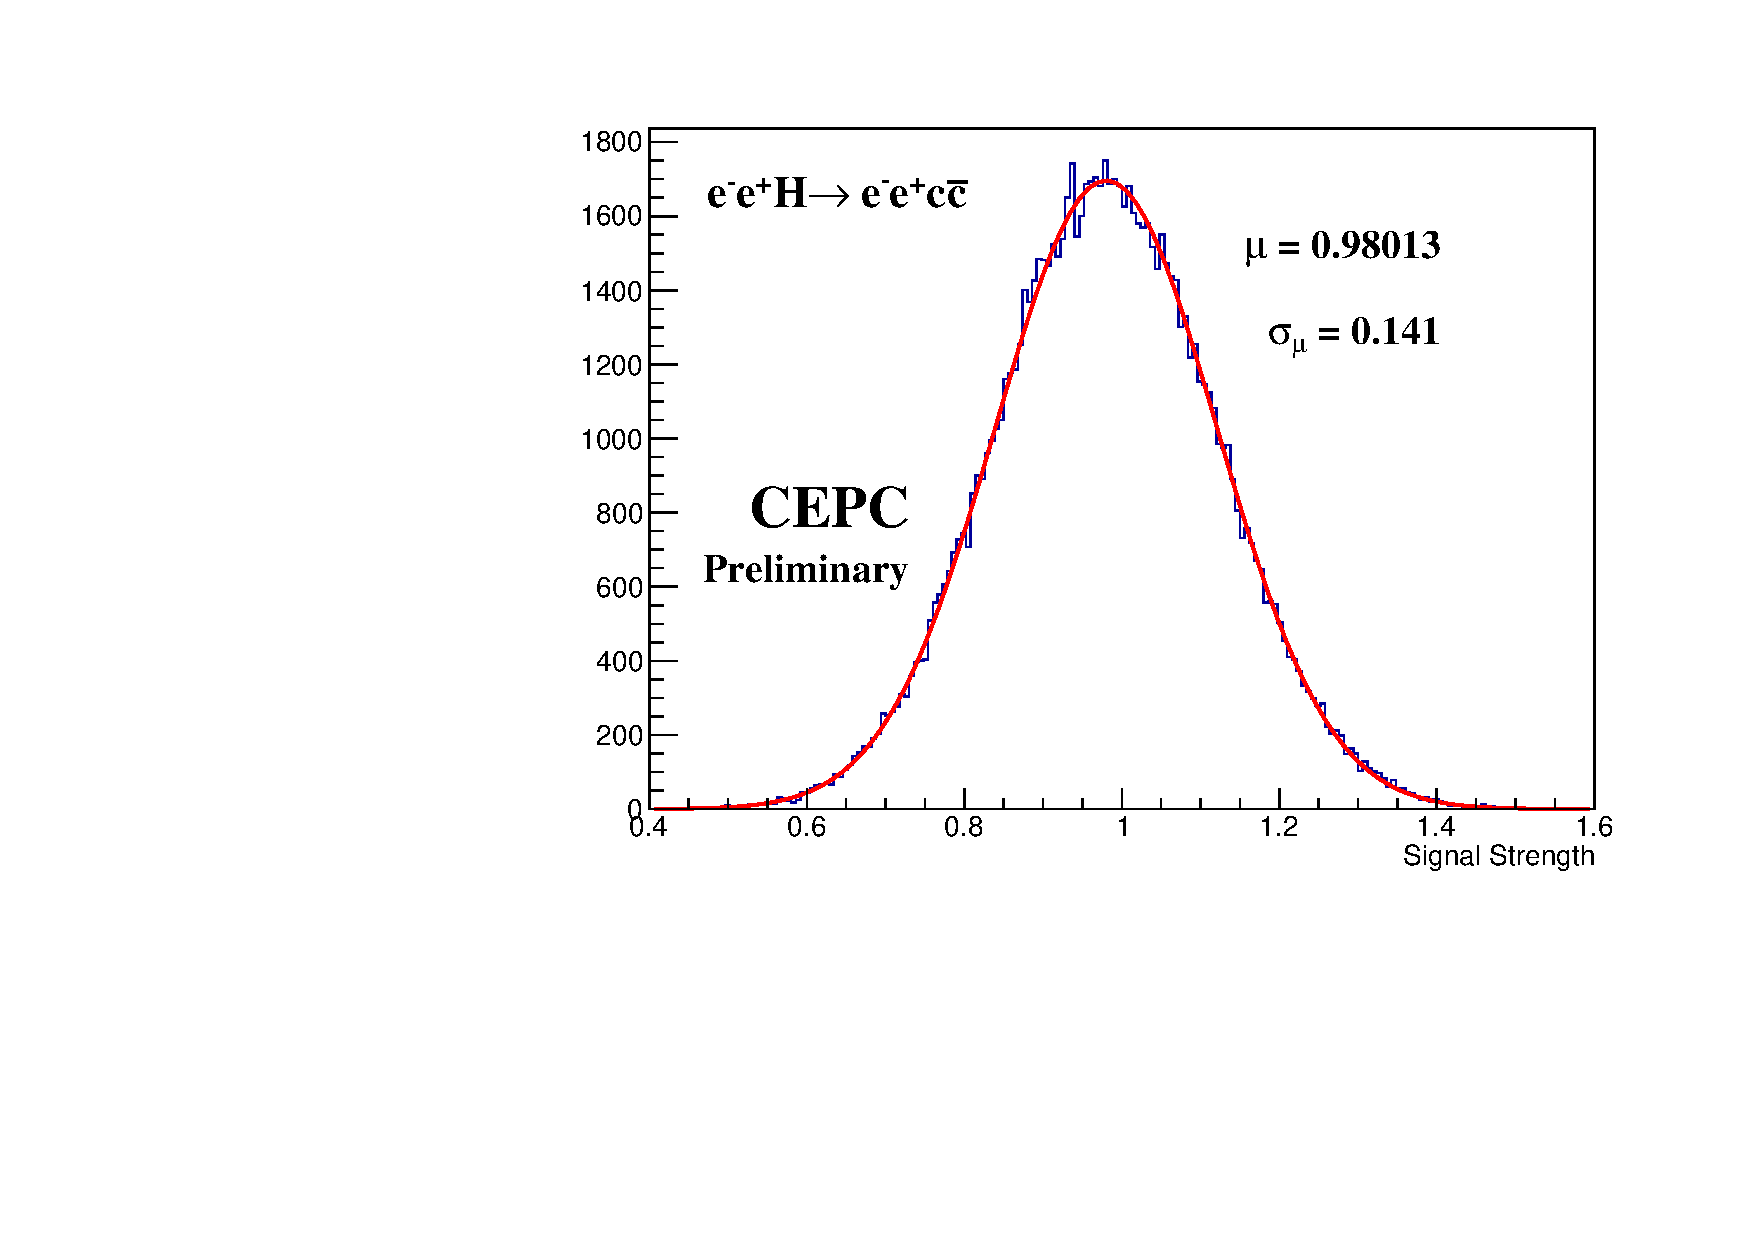
\includegraphics[width=\textwidth]{Template/toymc_eeh_cc.pdf}
     \end{minipage}
}
\subfigure[]
{
     \begin{minipage}[b]{0.31\textwidth}
     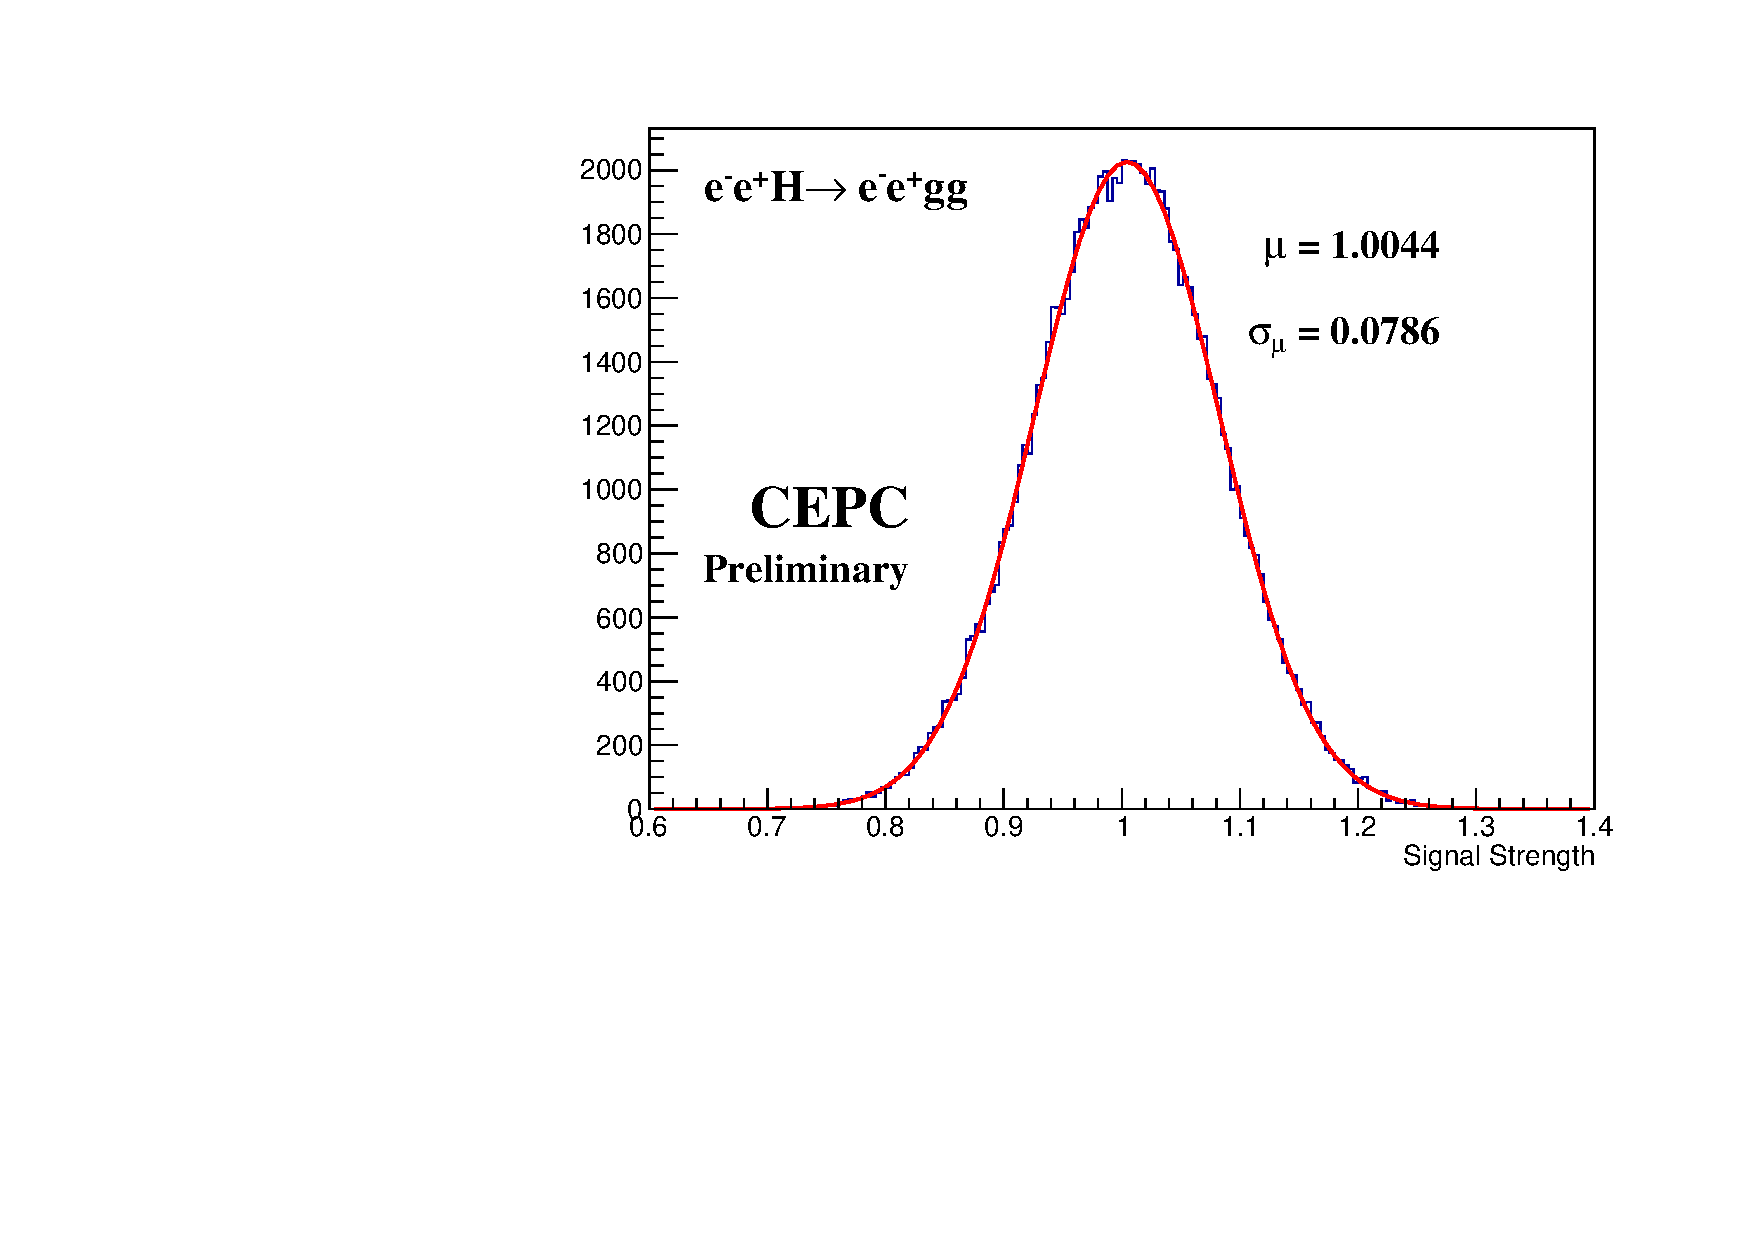
\includegraphics[width=\textwidth]{Template/toymc_eeh_gg.pdf}
     \end{minipage}
}
\subfigure[]
{
     \begin{minipage}[b]{0.31\textwidth}
     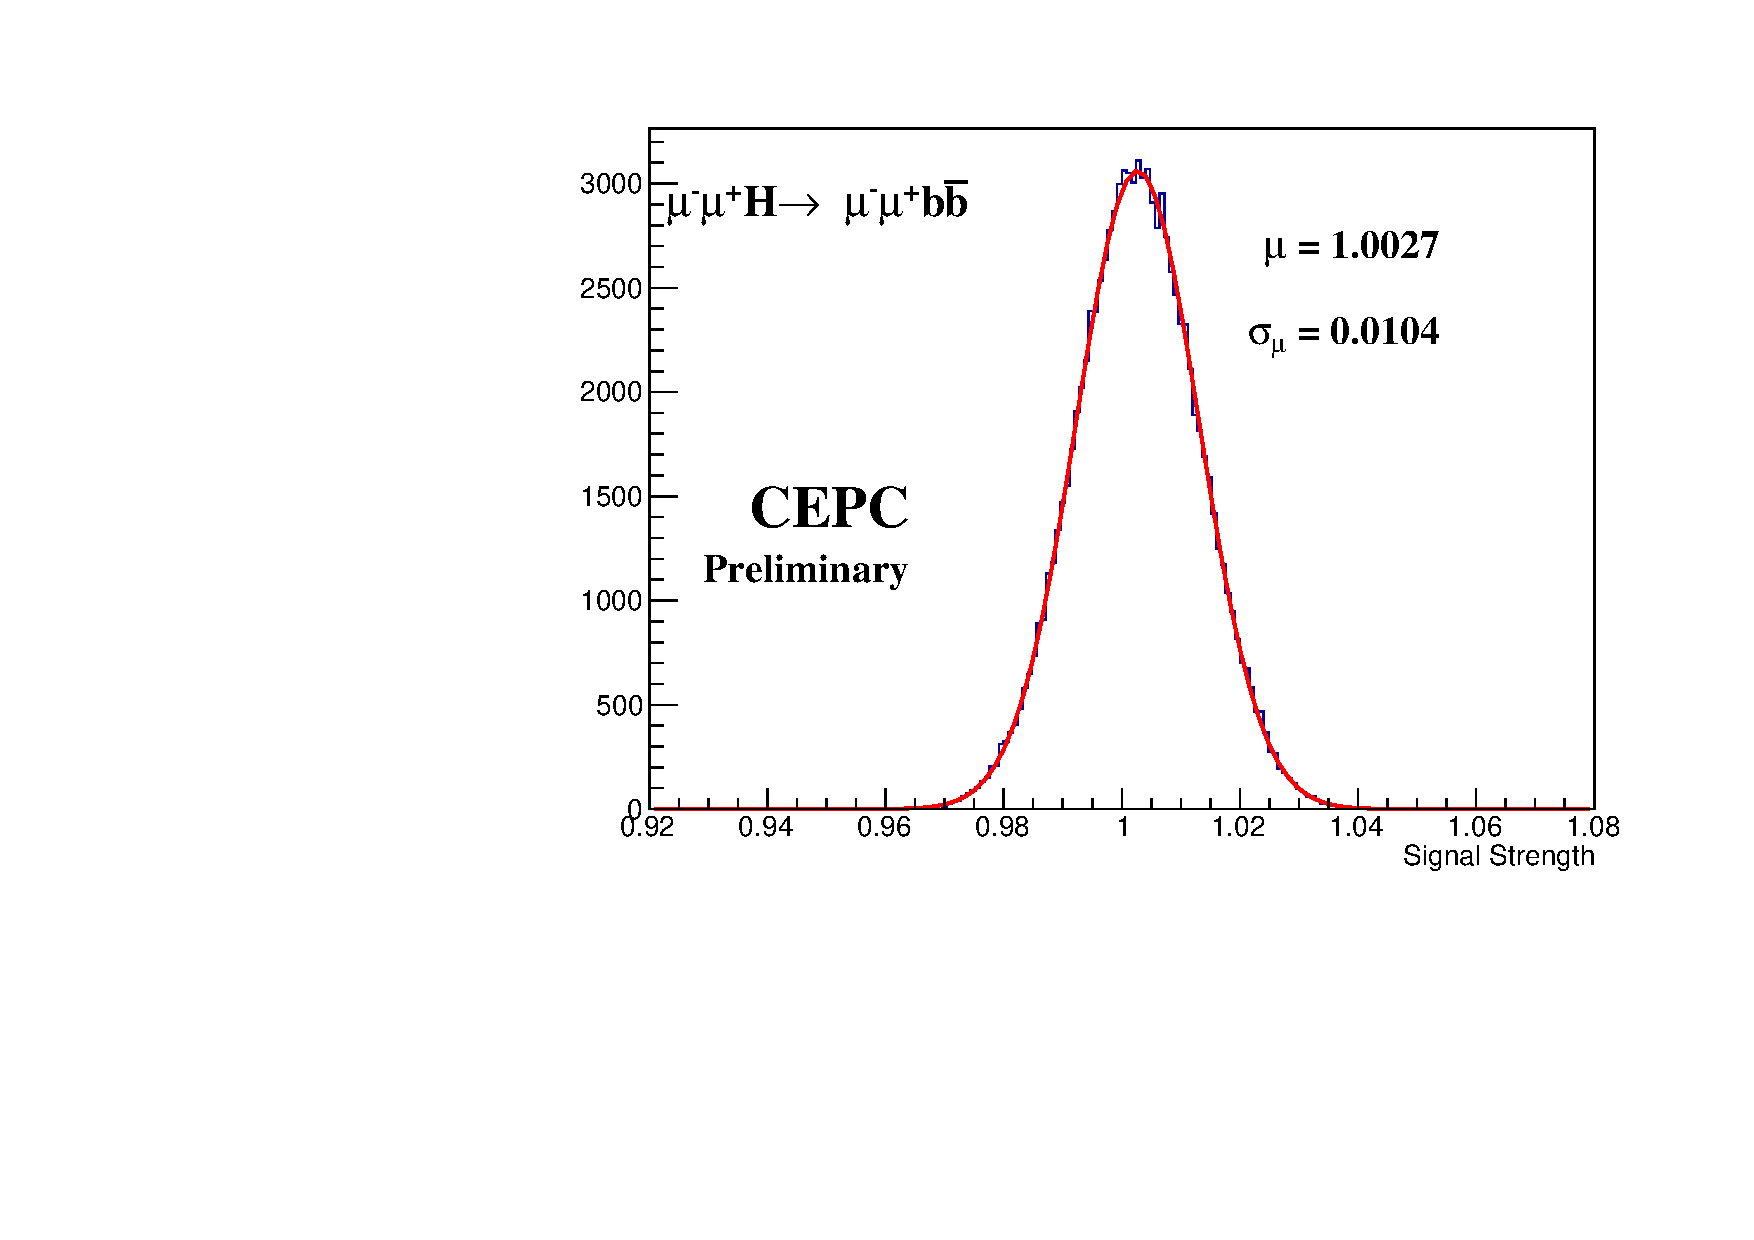
\includegraphics[width=\textwidth]{Template/toymc_mumuh_bb.pdf}
     \end{minipage}
}
\subfigure[]
{
     \begin{minipage}[b]{0.31\textwidth}
     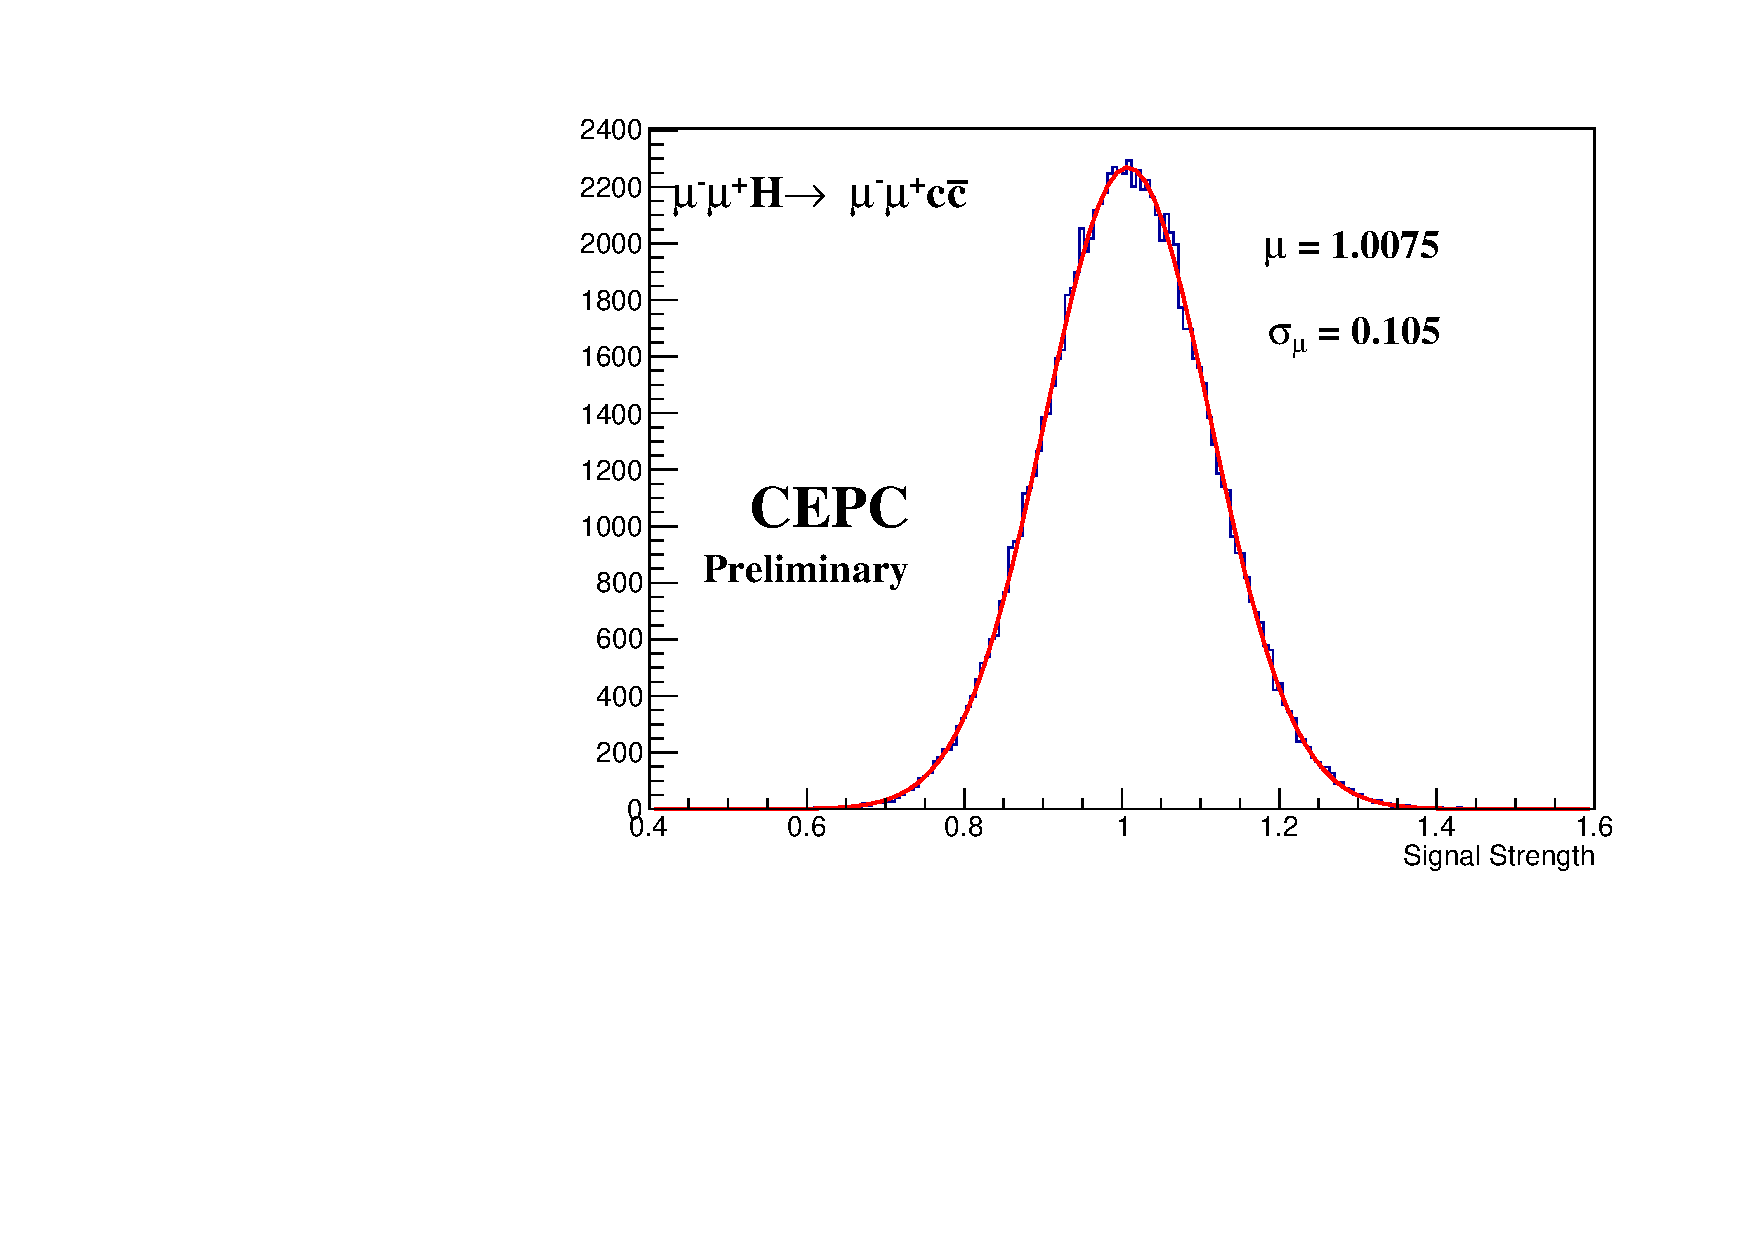
\includegraphics[width=\textwidth]{Template/toymc_mumuh_cc.pdf}
     \end{minipage}
}
\subfigure[]
{
     \begin{minipage}[b]{0.31\textwidth}
     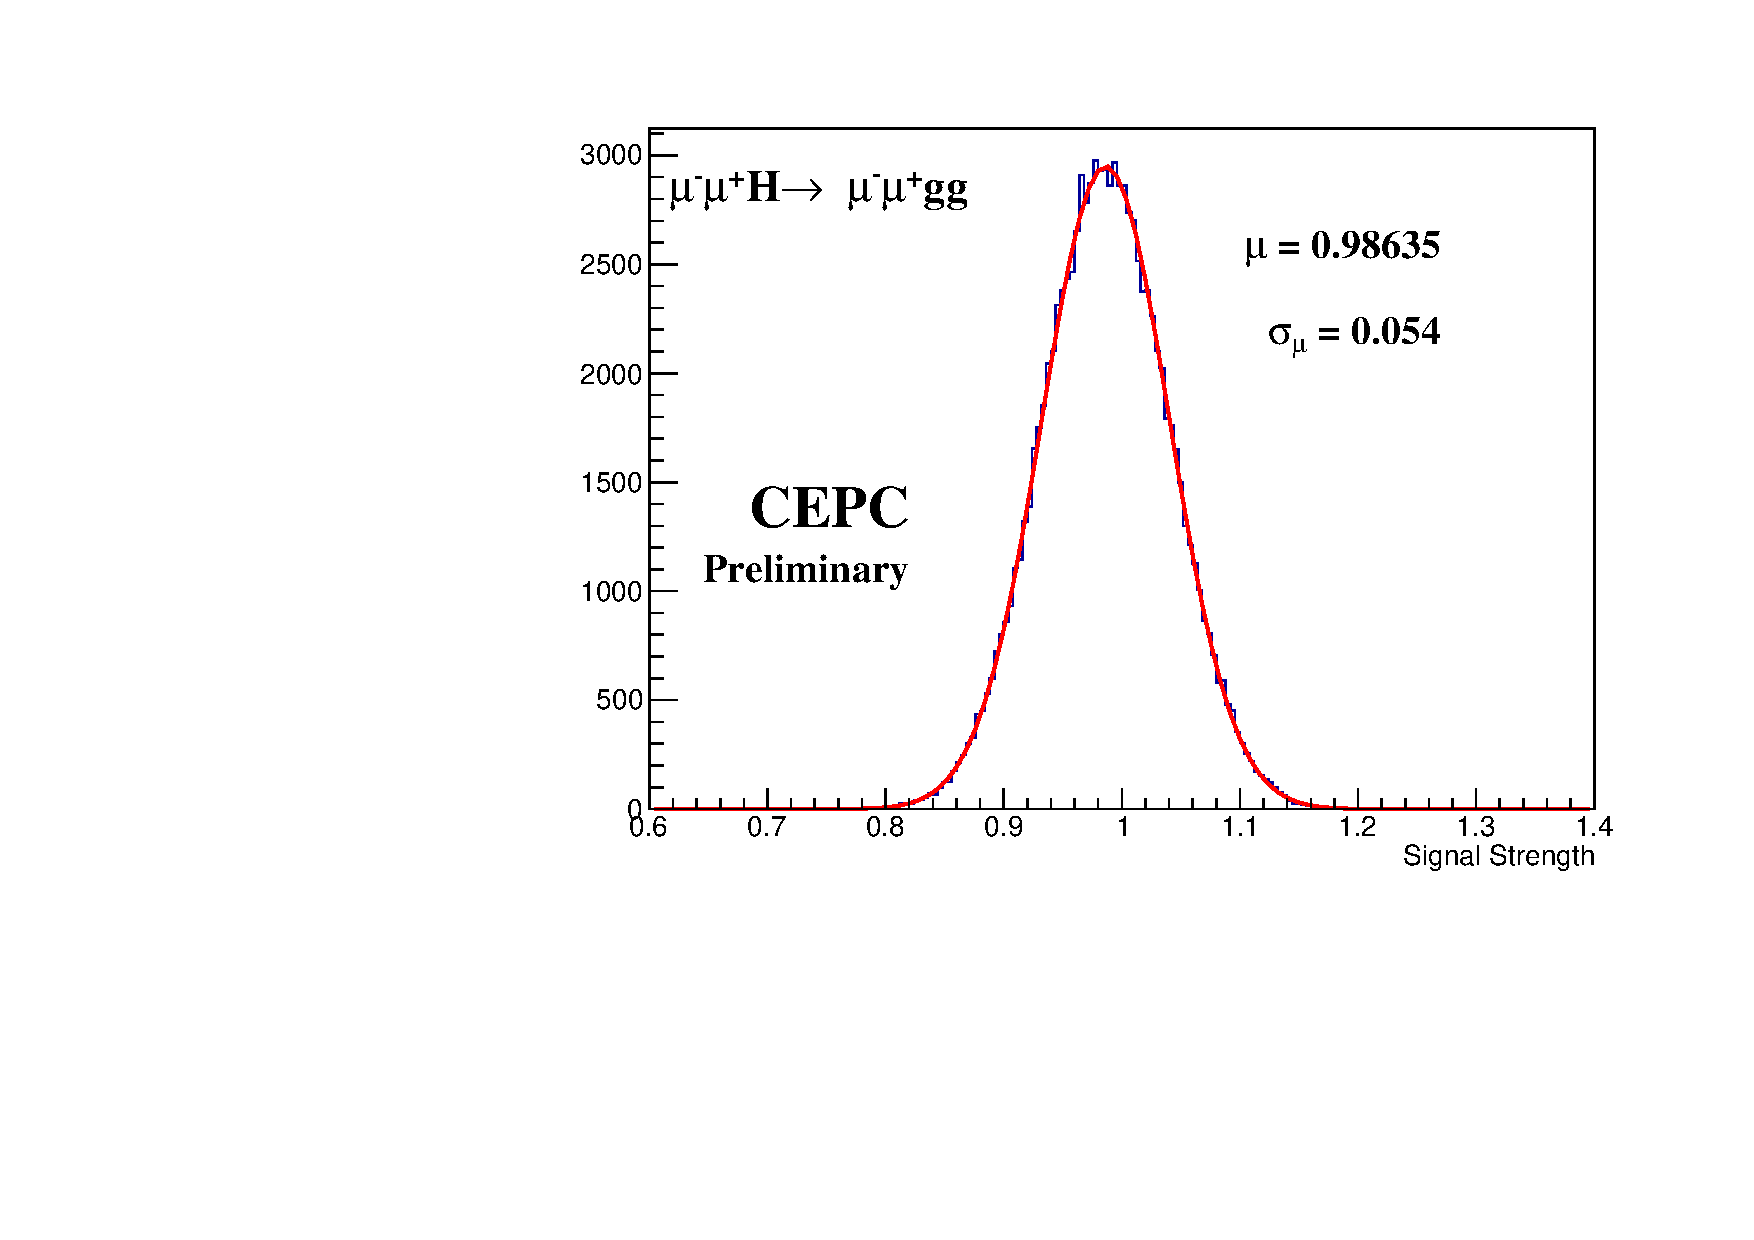
\includegraphics[width=\textwidth]{Template/toymc_mumuh_gg.pdf}
     \end{minipage}
}
\subfigure[]
{
     \begin{minipage}[b]{0.31\textwidth}
     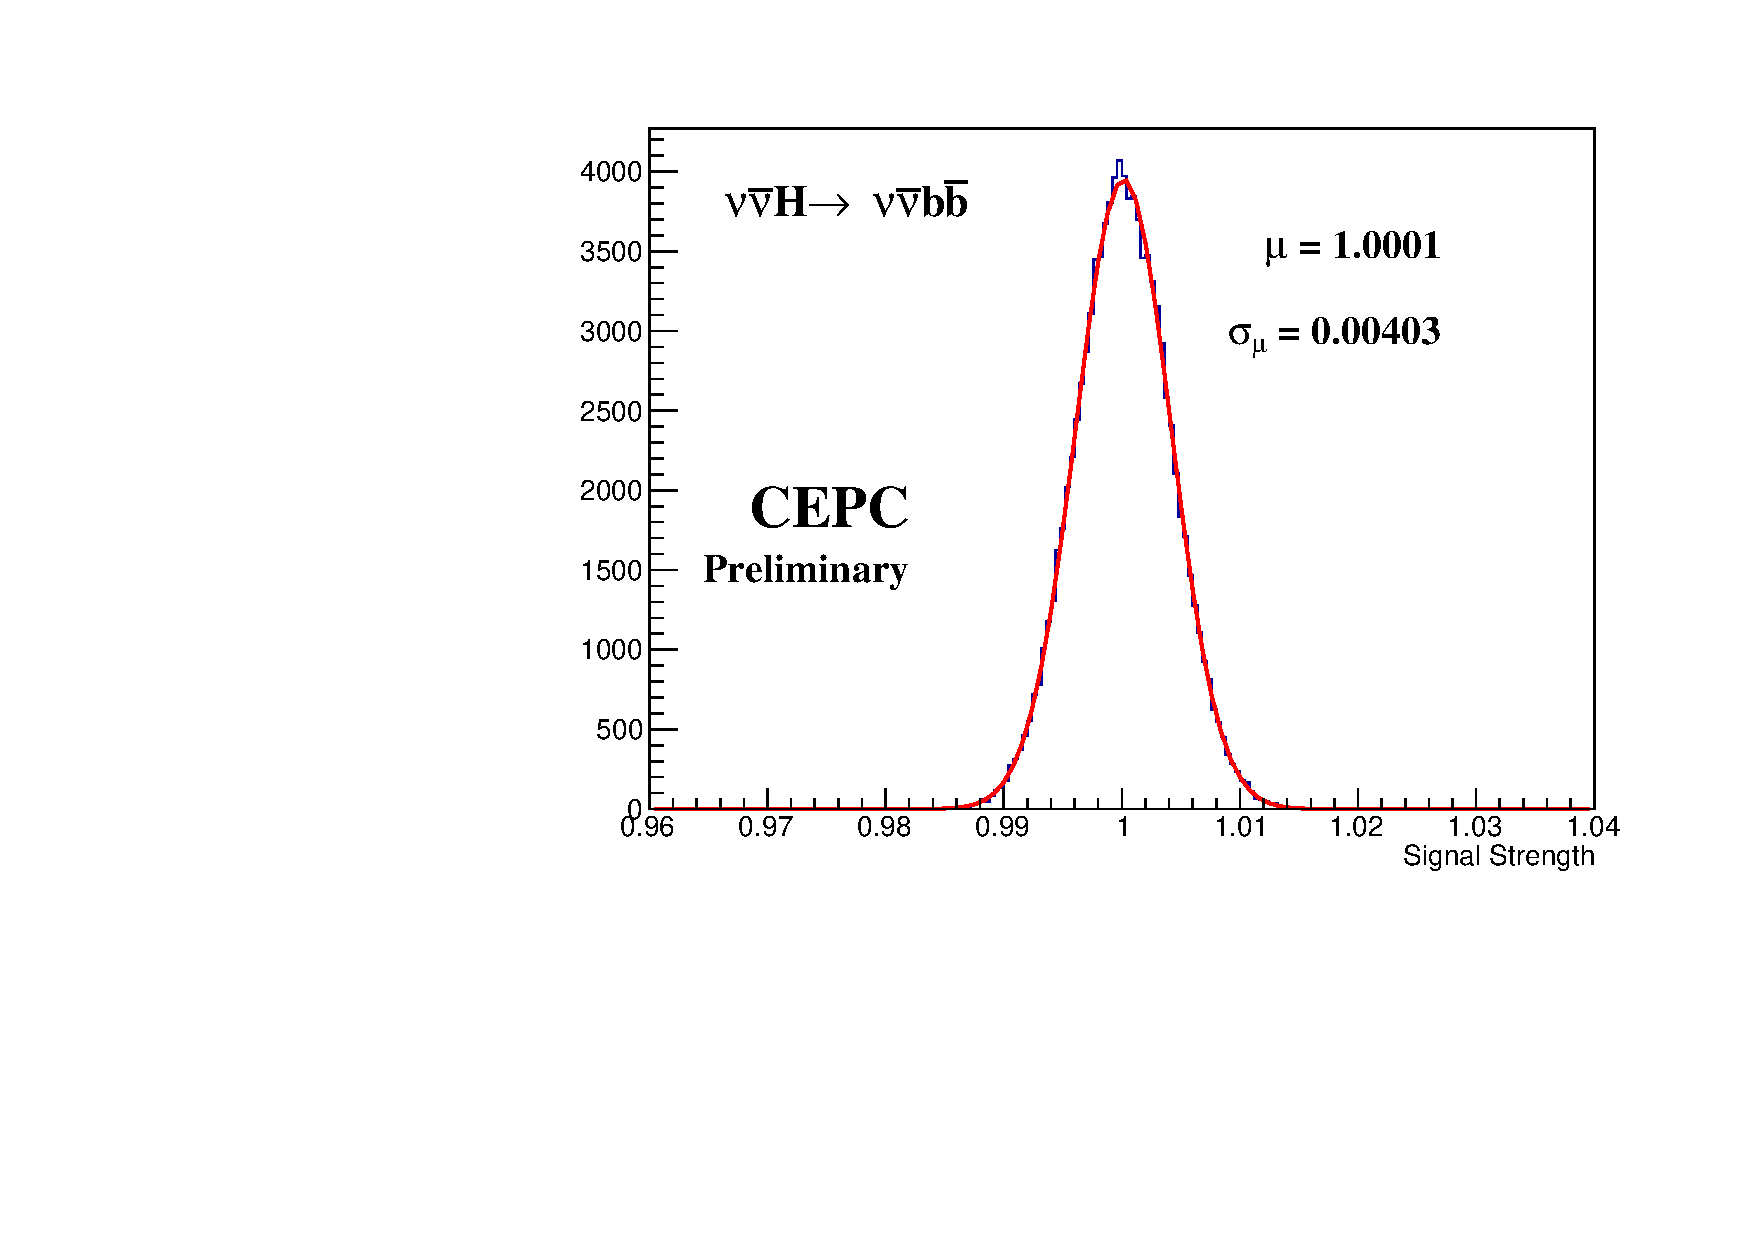
\includegraphics[width=\textwidth]{Template/toymc_nnh_bb.pdf}
     \end{minipage}
}
\subfigure[]
{
     \begin{minipage}[b]{0.31\textwidth}
     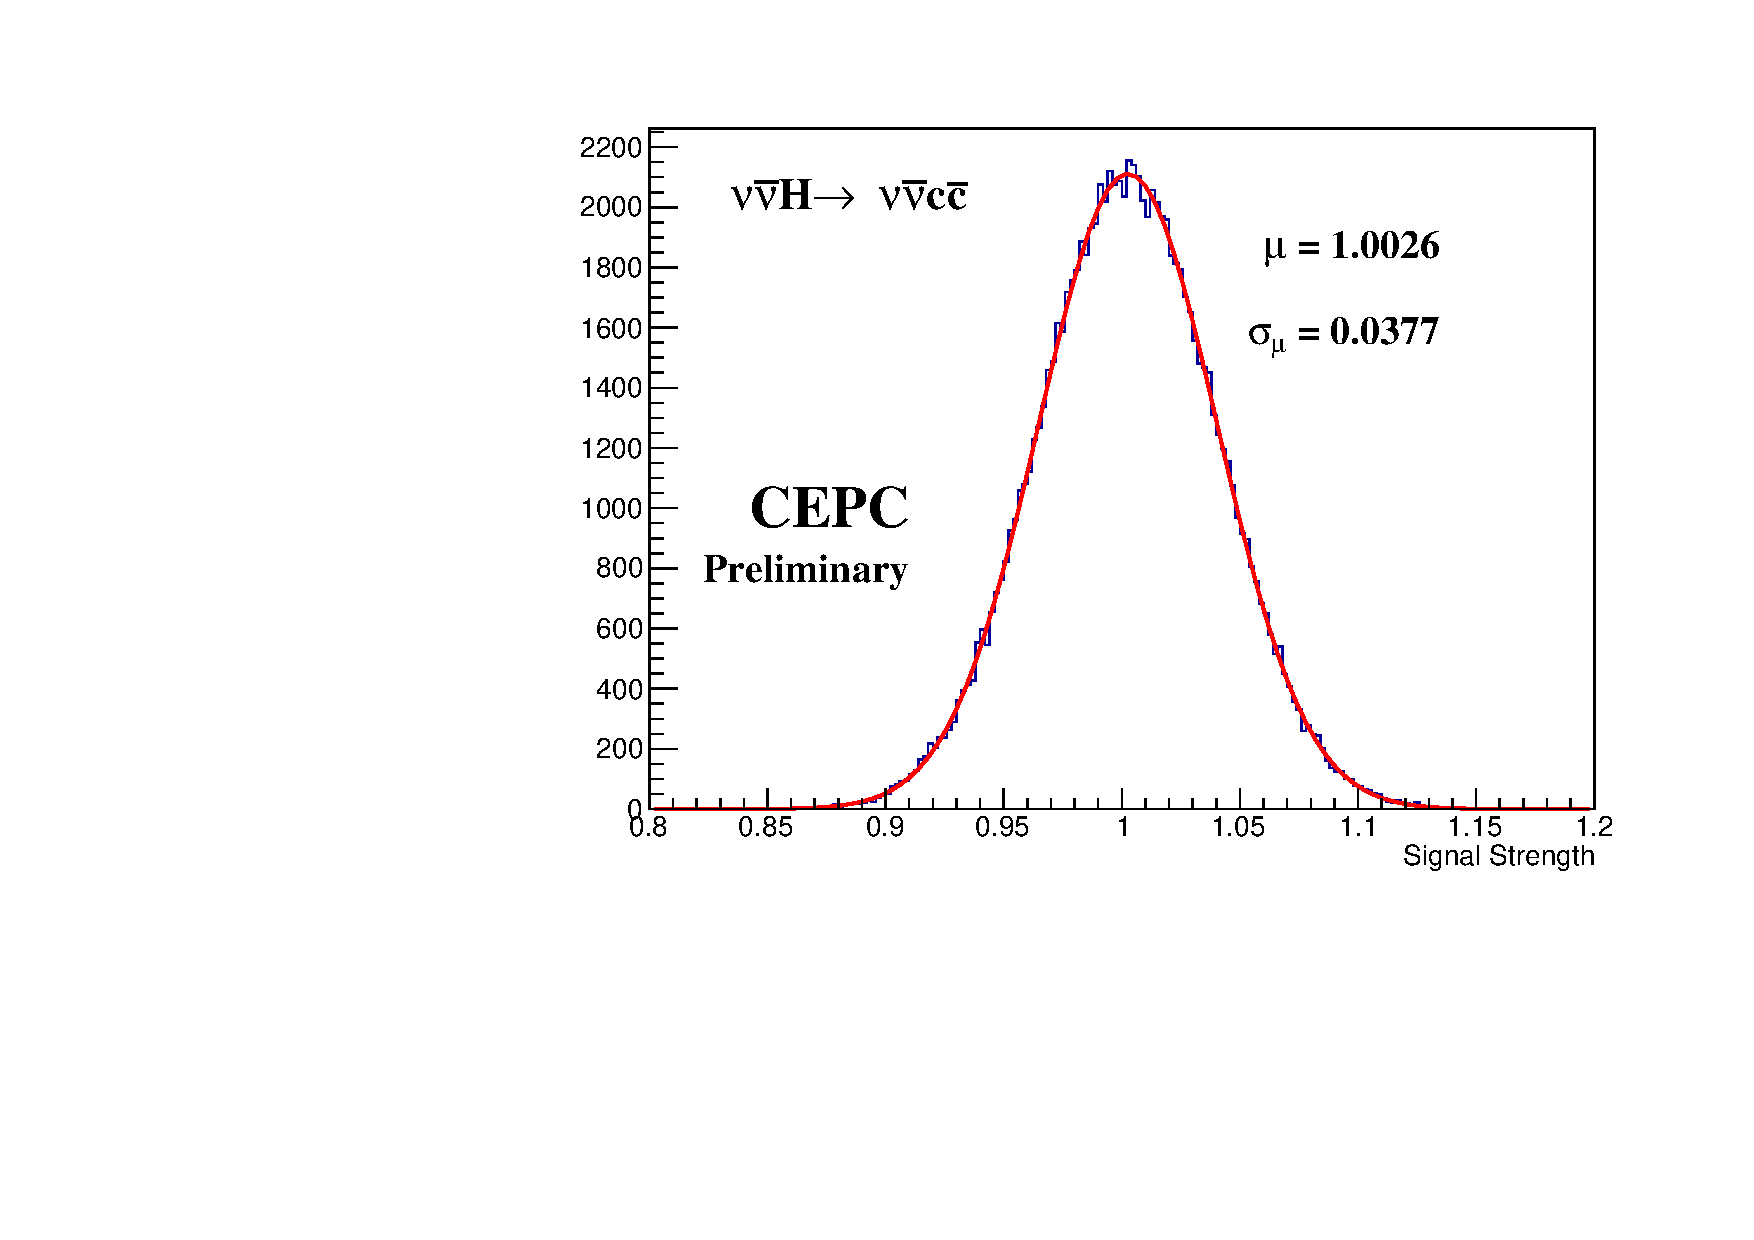
\includegraphics[width=\textwidth]{Template/toymc_nnh_cc.pdf}
     \end{minipage}
}
\subfigure[]
{
     \begin{minipage}[b]{0.31\textwidth}
     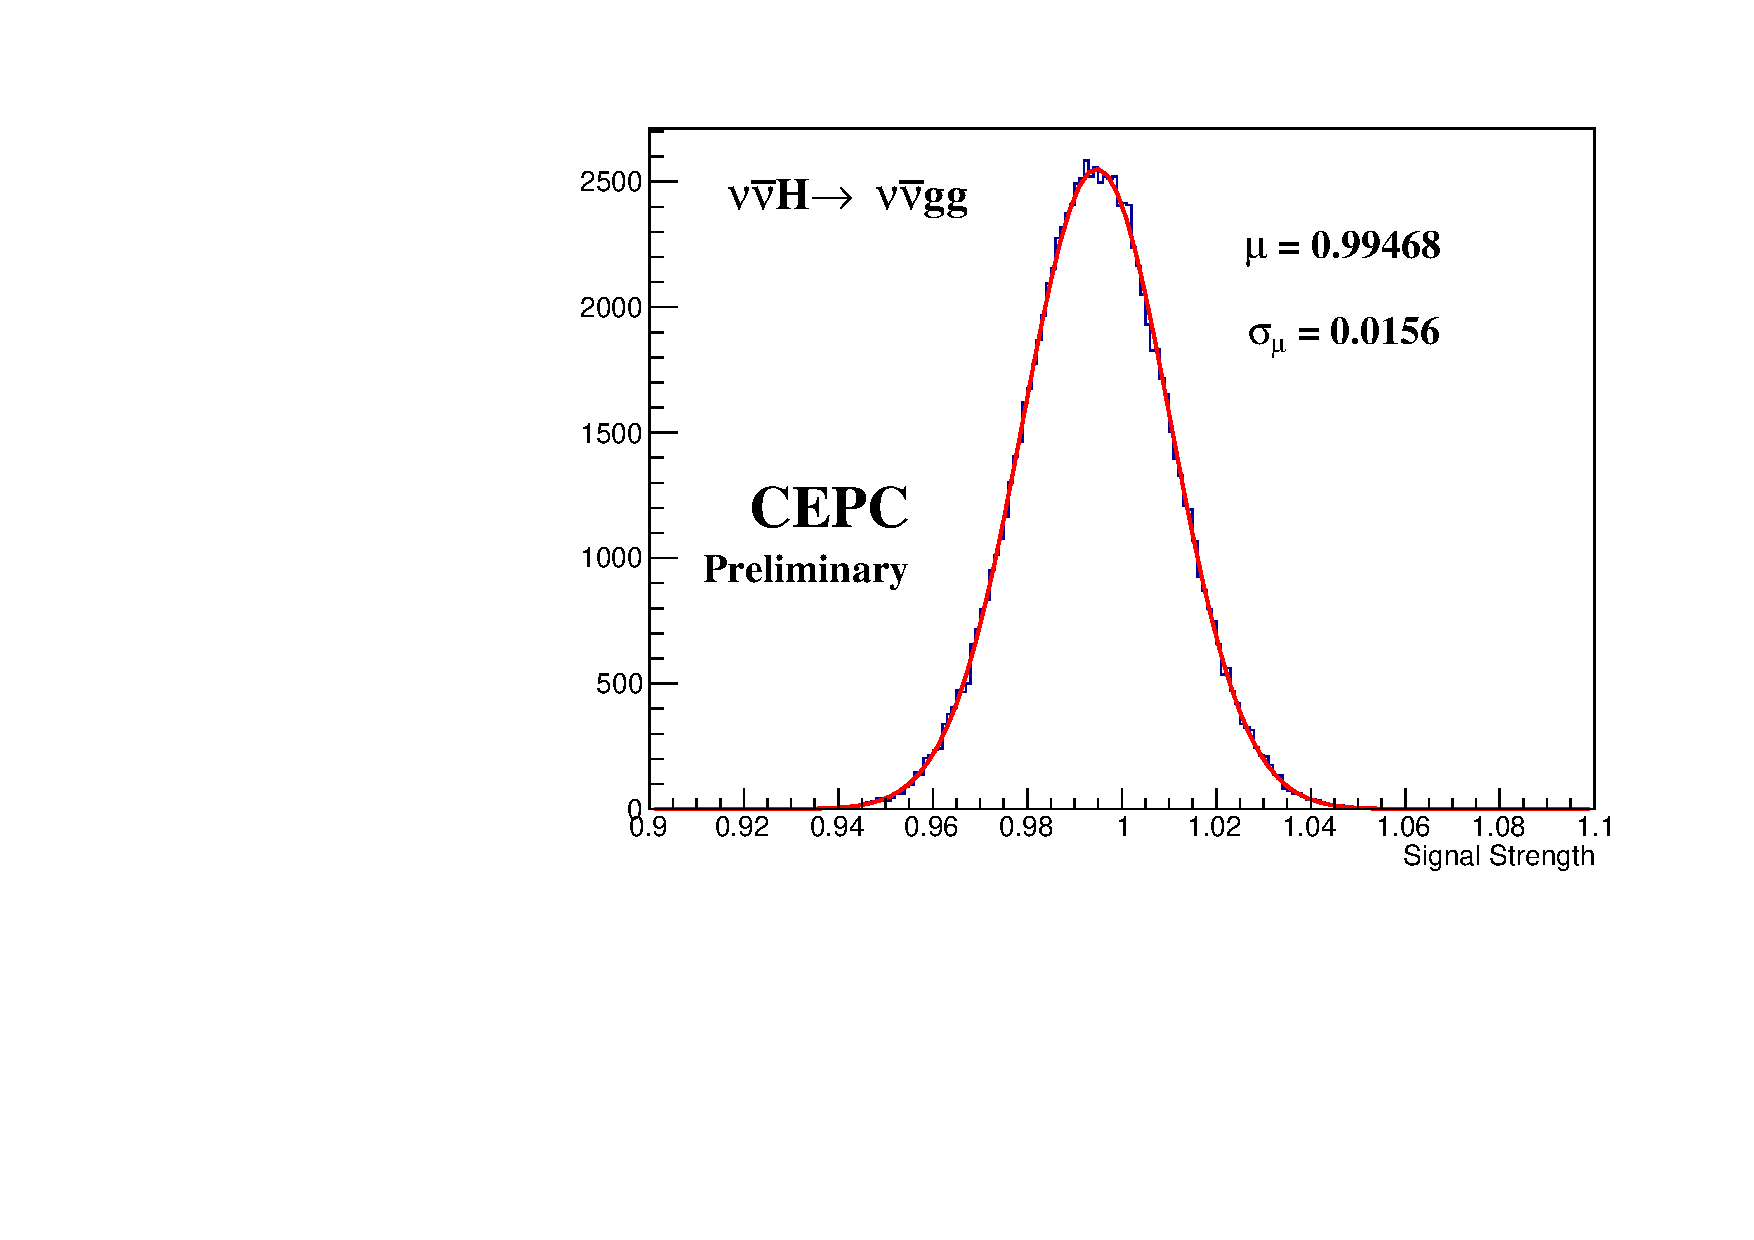
\includegraphics[width=\textwidth]{Template/toymc_nnh_gg.pdf}
     \end{minipage}
}
\subfigure[]
{
     \begin{minipage}[b]{0.31\textwidth}
     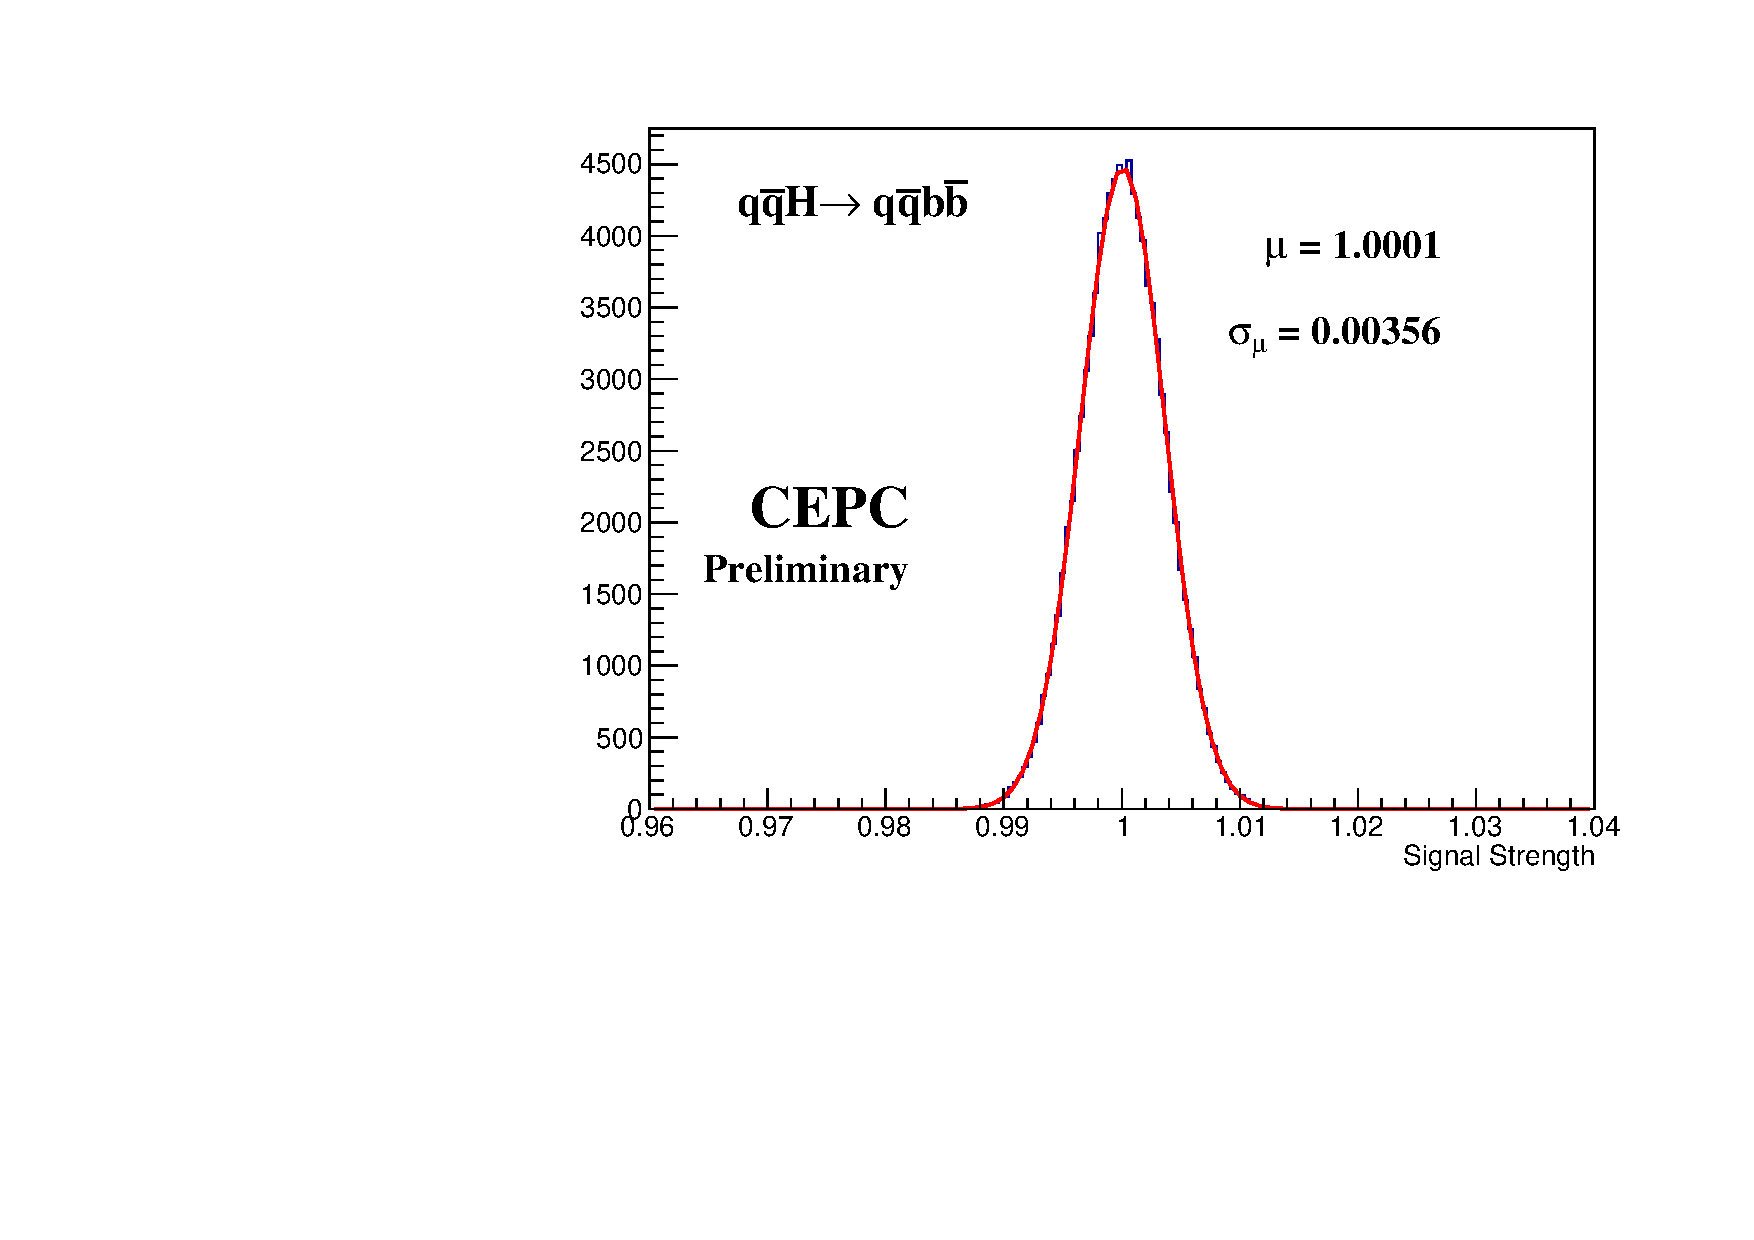
\includegraphics[width=\textwidth]{Template/toymc_qqh_bb.pdf}
     \end{minipage}
}
\subfigure[]
{
     \begin{minipage}[b]{0.31\textwidth}
     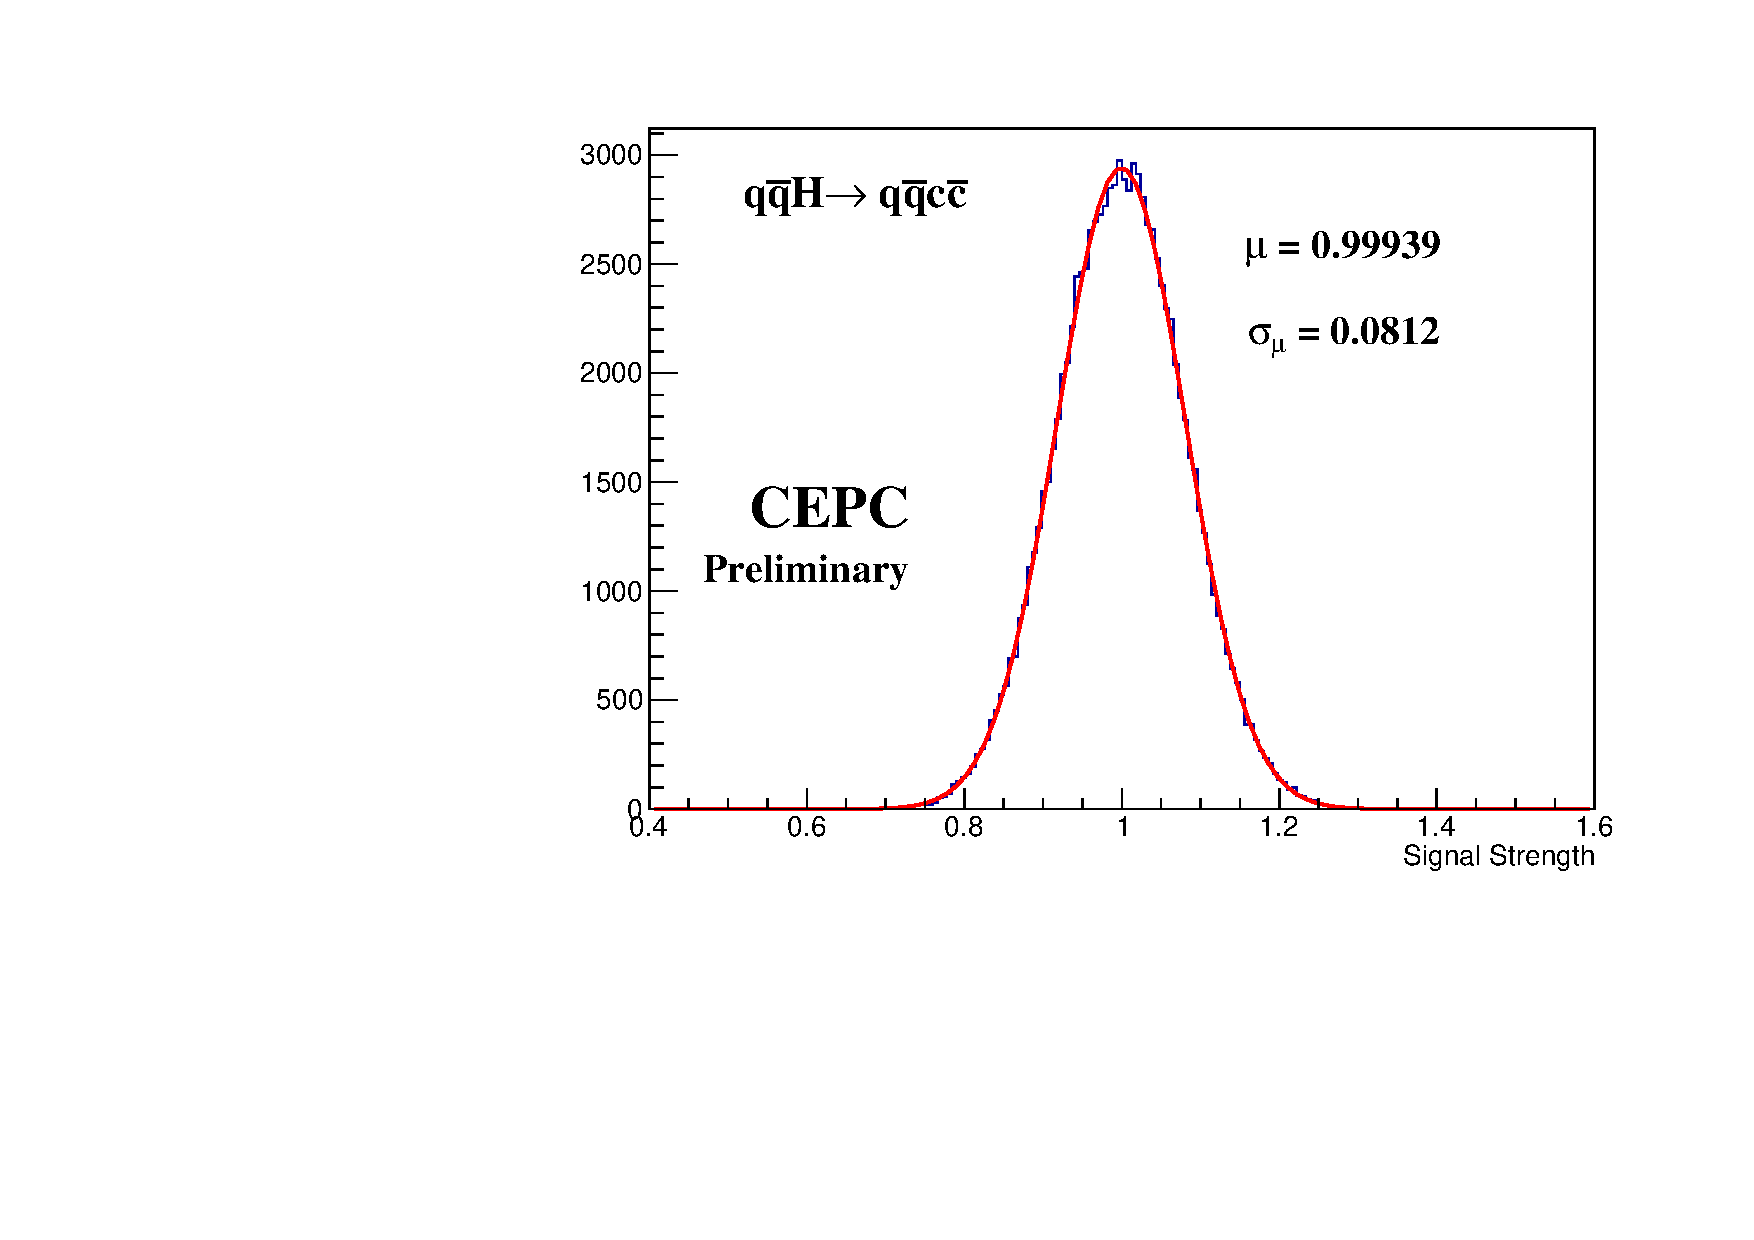
\includegraphics[width=\textwidth]{Template/toymc_qqh_cc.pdf}
     \end{minipage}
}
\subfigure[]
{
     \begin{minipage}[b]{0.31\textwidth}
     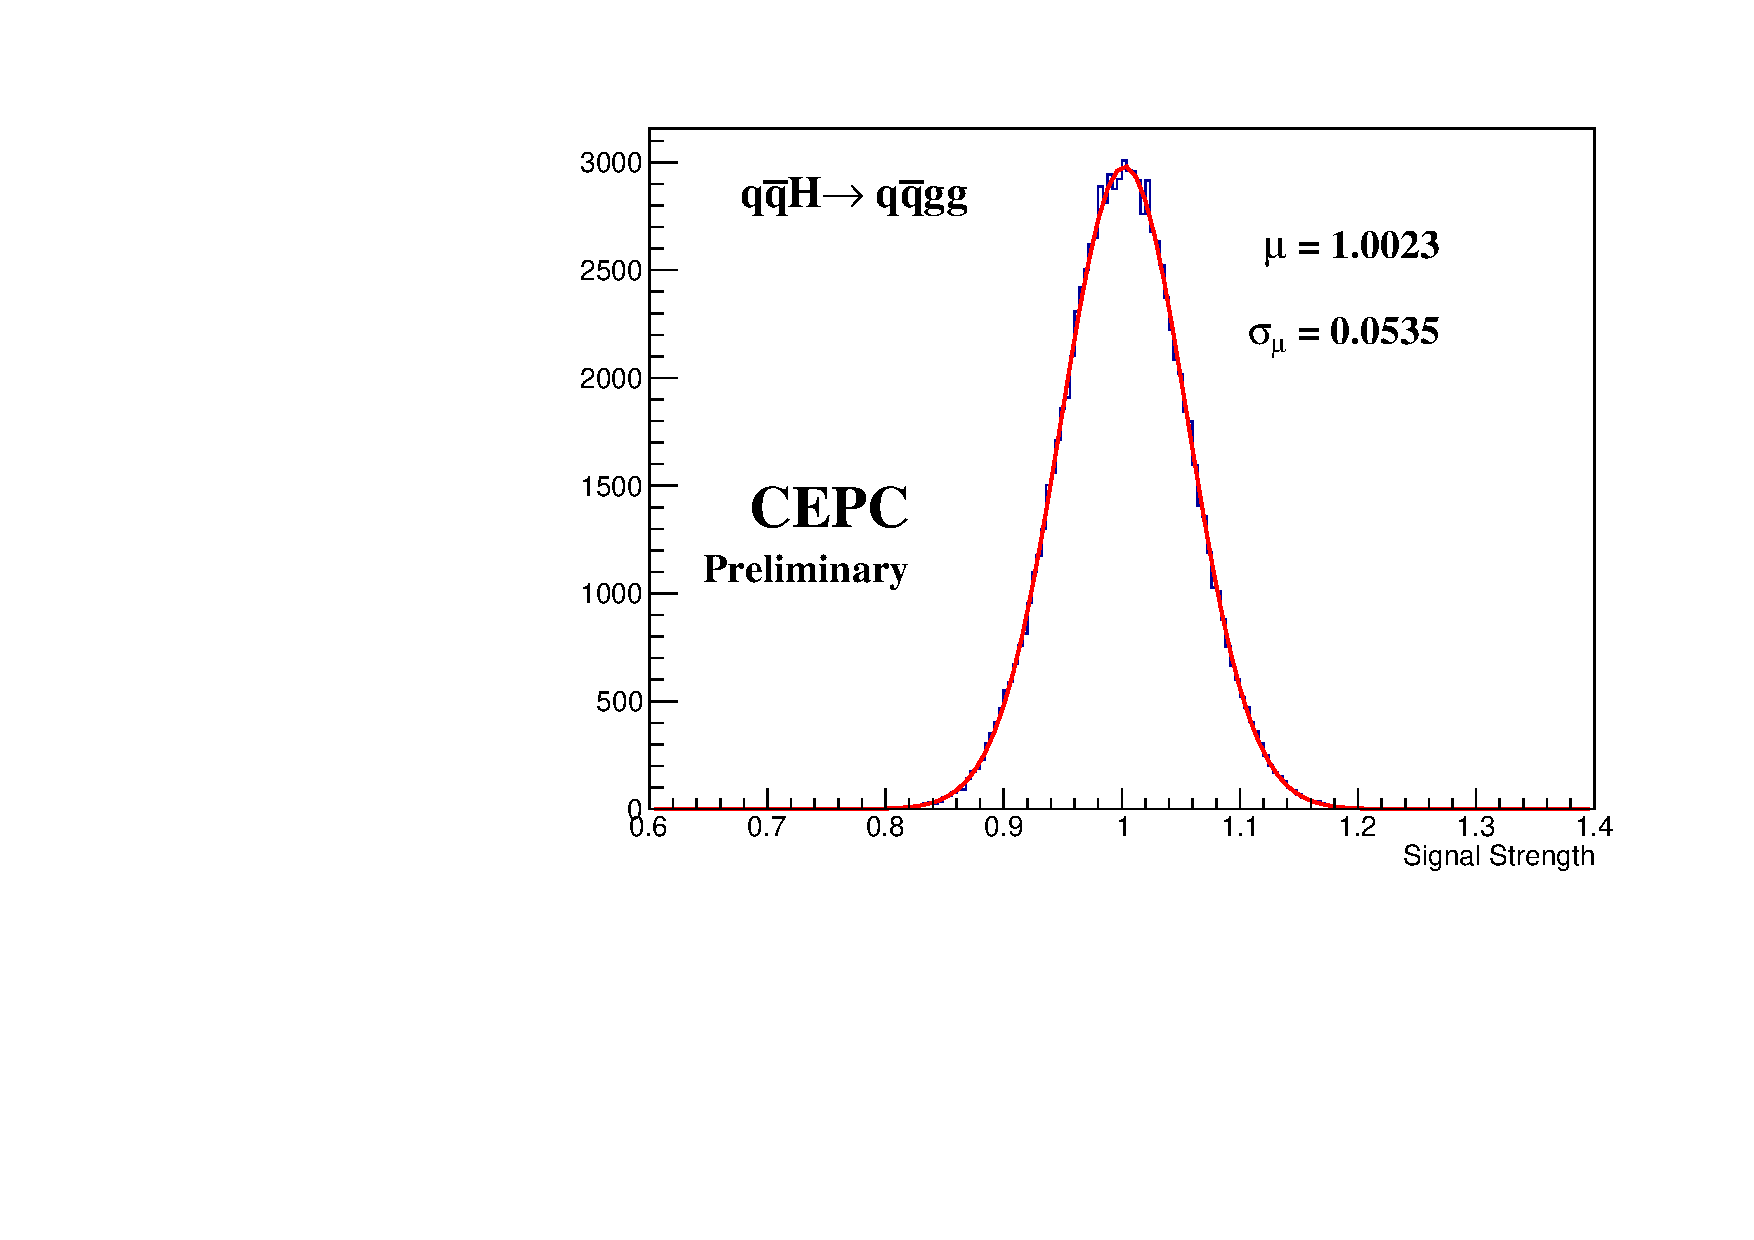
\includegraphics[width=\textwidth]{Template/toymc_qqh_gg.pdf}
     \end{minipage}
}
\caption{Toy MC test result in terms of signal strength and uncertainty from template fit. The signal strength from template fit in each channel for each higgs hadronic decay is presented. Plots in each row are from the same channel, from top row to bottom row are : \eeh, \mmh, \nnh and \qqh; plots in each column are from the same higgs decay mode, from left to right column are $H\rightarrow \bpair$, $H\rightarrow \cpair$ and $H\rightarrow \gpair$.}
\label{fig:toymc_subchannel}
\end{figure}

